\documentclass[oneside]{book}
\usepackage{verbatim}
\usepackage{fancyhdr}
\pagestyle{fancy}
\usepackage{graphicx}
\usepackage[font=small,labelsep=none]{caption}
\usepackage{listings}
%\usepackage{courier}
\lstset{language=PHP,
%frame=single,
%numbers=left,
basicstyle=\footnotesize\ttfamily,
tabsize=4,
showspaces=false,
showstringspaces=false
}

\fancyhead[LO,LE]{}
%\fancyhead[RC,RC]{}
%\fancyhead[RO,RE]{}

\fancyfoot[LO,LE]{Prepared for Robert Hoffner; Copyright \copyright 2011 Pulse Storm LLC}
\fancyfoot[RC,RC]{}
\fancyfoot[RO,RE]{\thepage}

\DeclareGraphicsExtensions{.pdf,.png,.jpg,.gif}

\usepackage{parskip}
\setlength{\parindent}{0pt}

\begin{document}

\title{No Frills Magento Layout}
\author{Alana Storm}
\date{April 2011}

\maketitle
\tableofcontents
\setcounter{chapter}{-1}

\chapter{No Frills Magento Layout: Introduction}
If you're reading this intro, chances are you know something about Magento.  Maybe you've chosen it for your new online store, maybe it's been chosen for you, or maybe you're just the curious type.  Whatever the reason you've kicked the tires, liked what you've seen, and ran to this book for help once you opened the hood.

Magento isn't \textbf{just} a shopping cart.  It's an entire system for programming web applications and performing system integrations.  The PHP you see here is not your your father's PHP.  It's probably not even your PHP.  Magento takes enterprise java patterns and applies them to the PHP language.  More than any system available today, it's pushing the limits of what's possible with object oriented PHP code.

When it comes to layout engines, Most PHP MVC systems use a simple outer-shell/inner-include approach.  Magento does not.  At the top of the Magento view layer there's a layout object, which controls a tree of nested block objects. Magento uses a domain specific programming language, implemented in XML, to create, configure, and render this nested tree of block objects into HTML.  This layer is separate from the rest of the application, allowing non-PHP developers an unprecedented level of power to change their layouts without having to touch a single line of PHP code.

If the above paragraph was greek to you don't worry, you're not alone.  With all that power available there's a learning curve to Magento that can be hard to climb by yourself.   This book is your guide up that learning curve.  We'll tell you what you need to know to quickly become a Magento Layout master.

\section{Who this Book is For}

This book is for interactive developers and software engineers who want to fully understand Magento's XML based Layout system.

By interactive developer we mean someone who both designs online experiences, and \textbf{implements} them using a mix of HTML/CSS/Javascript and some glue/template programming in a dynamic language like PHP, Ruby, Python, or one of those language's many template systems.  There are parts of the book where we'll dive in depth into how a particular system is built, but only so that you can better understand the context of where and when to use it.  Designer-coders are quickly taking over the agency world, and this book seeks to give them the tools they need to succeed.

Software engineer always seemed a fancier title than most jobs entail, so substitute software developer, or even PHP developer, if you're uncomfortable with engineer.  Chances are if you work for a shop that does more than just crank out web stores you're going to be asked to extend, enhance, and generally abuse Magento, including the Layout system.  In teaching you the practical, this book will also teach and inform on the engineering assumptions of the Layout system.  After reading through this book you'll not only understand how to use the Layout system, you'll understand why it was built the way it was, which in turn will help you make better engineering decisions on your own project.

This book assumes some basic PHP and Magento knowledge.  If you haven't already done so, reviewing the Magento Knowledge Base, as well as the additional articles on the author's website will help you get where you need to with Magento.

\begin{quote}
http://www.magentocommerce.com/knowledge-base

  http://alanastorm.com/category/magento
\end{quote}

You don't need to be a Magento master, but you should be passably familiar with the application.  If you aren't, you will be by the time you're done!  While the main text of the Book is focused on the Layout and related systems, whenever a deeper knowledge of Magento is needed the Appendixes will give you the overview you  need to keep working.

\section{No Frills}

Why No Frills?  Because we tell you what you need to know, and nothing more.  Mandated book lengths make sense in a physical retail environment, but with the internet being the preferred way of distributing technical prose, there's no need to pad things out.

With that in mind, lets get started!

\section{Installing Modules}

This book was distributed with an archive containing several versions of a Magento module named \footnotesize\texttt{Nofrills\_Booklayout}\normalsize.  If you want to add code to a Magento system, you create a module.  The \footnotesize\texttt{Nofrills\_Booklayout} \normalsize  module is where the example code in this book will go.  You'll be building this module up as you go along.  For each chapter in the book, we've included the module as it should be at the start of the chapter, and how it should be at the end.

You'll also find a copy of each and every code example in the \footnotesize\texttt{code/all} \normalsize  folder. If you don't want to manually type in code examples from the book, copy and paste the contents of these files into your source code editor.

There are two ways to install the module.  The first is manually.  If you extract the files, you'll see a folder structure like

\begin{lstlisting}
app/code/local/Nofrills_Magento
app/module/etc/Nofrills_Magento.xml
app/.....

\end{lstlisting}


The archive structure mirrors where the files should be placed in your system.  This is the standard layout of a Magento extension.  Place the files in the same location on your own installation, clear your cache, and the extension will be loaded into the system on the next page request. For more background, read the Magento Controller Dispatch and Hello World article online

\begin{quote}
http://alanastorm.com/magento\_controller\_hello\_world
\end{quote}

If you're not up for a manual install, each archive is also a fully valid Magento Connect package.  Magento Connect is Magento Inc's online marketplace of free extensions.  It's also a package management system.  For background on Magento Connect and instructions for installing its packages, please see Appendix J.

\section{Parting Words}

A few last things before we start.  Magento has a special operating mode called \footnotesize\texttt{DEVELOPER\_MODE}\normalsize.  When running in \footnotesize\texttt{DEVELOPER\_MODE} \normalsize  Magento is less tolerant of small coding errors, and will not hide fatal errors and uncaught exceptions from the end user.  You'd never want to run a production store in \footnotesize\texttt{DEVELOPER\_MODE}\normalsize, but it can make working with and learning the system much easier.  You'll want to turn \footnotesize\texttt{DEVELOPER\_MODE} \normalsize  on while working your way through this book.  You can do this by either

\begin{enumerate}
\item Adding \footnotesize\texttt{SetEnv MAGE\_IS\_DEVELOPER\_MODE 1} \normalsize  to your .htaccess file
\item Alternately, editing \footnotesize\texttt{index.php} \normalsize
\end{enumerate}


If you choose the second option, look for lines in your \footnotesize\texttt{index.php} \normalsize  file something like

\begin{lstlisting}
if (isset($_SERVER['MAGE_IS_DEVELOPER_MODE'])) {
    Mage::setIsDeveloperMode(true);
}

\end{lstlisting}


You'll want to make sure the \footnotesize\texttt{Mage::setIsDeveloperMode(true);} \normalsize  call is made.  Also, while you're in \footnotesize\texttt{index.php}\normalsize, it'd be a good idea to tell PHP to show errors by changing this

\begin{lstlisting}
#ini_set('display_errors', 1);

\end{lstlisting}


to this

\begin{lstlisting}
ini_set('display_errors', 1);

\end{lstlisting}


Seemingly invisible errors are one of the most frusting things for a developer new to any system.  By configuring Magento to fail fast we'll be setting ourselves up to better learn what needs to be done for any given task.

Magento's a fast changing platform, and while the concepts in this book will apply to all versions the specifics may change as Magento Inc changes its focus.  It should go without saying you should run the exercises presented here on a development or testing server, and \textbf{not} your production environment.  The following legal notice is the fancy way of saying that

\begin{lstlisting}
THIS BOOK AND SOFTWARE IS PROVIDED BY THE COPYRIGHT HOLDERS AND
CONTRIBUTORS "AS IS" AND ANY EXPRESS OR IMPLIED WARRANTIES,
INCLUDING, BUT NOT LIMITED TO, THE IMPLIED WARRANTIES OF
MERCHANTABILITY AND FITNESS FOR A PARTICULAR PURPOSE ARE
DISCLAIMED. IN NO EVENT SHALL THE COPYRIGHT HOLDER OR CONTRIBUTORS
BE LIABLE FOR ANY DIRECT, INDIRECT, INCIDENTAL, SPECIAL,
EXEMPLARY, OR CONSEQUENTIAL DAMAGES (INCLUDING, BUT NOT LIMITED
TO, PROCUREMENT OF SUBSTITUTE GOODS OR SERVICES; LOSS OF USE,
DATA, OR PROFITS; OR BUSINESS INTERRUPTION) HOWEVER CAUSED AND ON
ANY THEORY OF LIABILITY, WHETHER IN CONTRACT, STRICT LIABILITY, OR
TORT (INCLUDING NEGLIGENCE OR OTHERWISE) ARISING IN ANY WAY OUT OF
THE USE OF THIS BOOK AND SOFTWARE, EVEN IF ADVISED OF THE
POSSIBILITY OF SUCH DAMAGE.

\end{lstlisting}


\section{Bugs in the Book}

If you're having trouble working your way through the examples, post a detailed question to the programming Q\&A site Stack Overflow

\begin{quote}
http://stackoverflow.com/tags/magento
\end{quote}

with the following tags

\begin{lstlisting}
magento magento-nofrills

\end{lstlisting}


We'll be monitoring the site for any problems with code examples, and by asking your questions in a public forum you'll be helping the global Magento developer community.  Developers are often amazed when they find people across the world are having the same problems they are, and often already have a solution ready to share.

Additionally, each chapter will contain a link to a site online for discussions specific to each chapter.  You're not just getting a book, you're joining a community.

\section{About the Author}

No Frills Magento Layout was written by Alana Storm.  Alana's an industry veteran with over 12 years on-the-job experience, and an active member of the Magento community.  He's written the go-to developer documentation for the Magento Knowledge Base, and is the author of the popular debugging extension Commerce Bug.  You can read more about Alana and her Magento products at the following URLs

\begin{quote}
http://alanastorm.com/

  http://store.pulsestorm.net/
\end{quote}

\section{Let's Go}

That's it for pleasantries, let's get started.  In the first chapter we're going to start by creating Magento layouts using PHP code.

\emph{Visit http://www.pulsestorm.net/nofrills-layout-introduction to join the discussion online.}
\chapter{Building Layouts Programmatically}
Before we can understand the layout system in its entirety, we need to understand its individual parts. With that in mind, we'll start with some simple examples.  A Layout can be defined with the following phrase

\begin{quote}
A Layout is a collection of blocks in a tree structure
\end{quote}

So, let's start by defining what a block is.

A Magento block is an object with a \footnotesize\texttt{toHtml} \normalsize  method defined.  When this \footnotesize\texttt{toHtml} \normalsize  method is called, it returns the string which should be output to the screen. Typically "the screen" means your web browser.  In addition to having a \footnotesize\texttt{toHtml} \normalsize  method, Magento blocks inherit from the \footnotesize\texttt{Mage\_Core\_Block\_Abstract} \normalsize  class. This class contains a number of other useful block helper methods.  We'll get to these eventually, but for now just think of a block as \textbf{an object} which has a \textbf{\footnotesize\texttt{toHtml} \normalsize } method, and when this \footnotesize\texttt{toHtml} \normalsize  is called \textbf{output is sent to the screen}.

Let's give this a try. If you installed the \footnotesize\texttt{Nofrills\_Booklayout} \normalsize  module that came with this book, you can open the following url on your system

\begin{quote}
http://magento.example.com/nofrills\_booklayout/index/index
\end{quote}

which corresponds to the controller file at

\begin{lstlisting}
app/code/local/Nofrills/Booklayout/controllers/IndexController.php

\end{lstlisting}


We'll be adding our code examples to the indexAction method

\begin{lstlisting}
public function indexAction()
{
    var_dump(__METHOD__);
}

\end{lstlisting}


If you load the above URL with an unmodified extension, you should see a mostly blank browser screen that looks something like \emph{Figure 1.1}

\begin{figure}[htb]
\begin{center}
\leavevmode
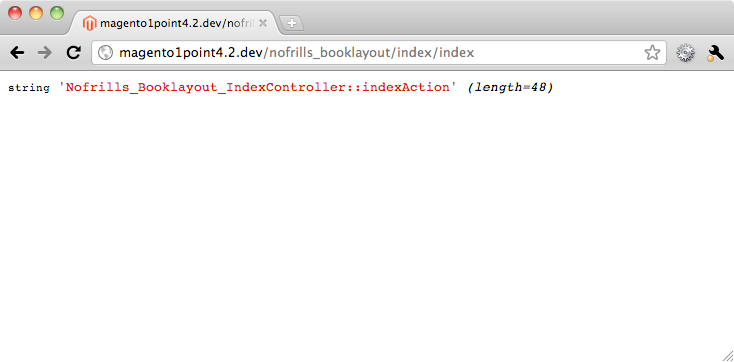
\includegraphics[width=1\textwidth]{images/chapter1/start.png}
\end{center}
\caption{}
%\label{fig:awesome_image}
\end{figure}


First, we'll create a simple text block.

\begin{lstlisting}
public function indexAction()
{
    $block = new Mage_Core_Block_Text();
    $block->setText("Hello World");
    echo $block->toHtml();
}

\end{lstlisting}


Our first line instantiates a block object from the class \footnotesize\texttt{Mage\_Core\_Block\_Text}\normalsize.  Our second line sets the text we want to output, and the third line calls the \footnotesize\texttt{toHtml} \normalsize  method, which returns our string and echos the output.

If you reload your browser page, you should see the following output.

\begin{lstlisting}
Hello World

\end{lstlisting}


So far so good. We now have an object oriented echo statement. In our example above we instantiated a \footnotesize\texttt{Mage\_Core\_Block\_Text} \normalsize  object. When you call this type of block's \footnotesize\texttt{toHtml} \normalsize  method, it simply outputs whatever text has been set with the \footnotesize\texttt{setText} \normalsize  method.

Magento has literally hundreds of different types of block classes for every possible need. The Magento core team subscribes to a style of development that's similar to Java and C\# programming that says

\begin{quote}
When in doubt, make a new class
\end{quote}

Each block type may have a slightly different implementation of how its \footnotesize\texttt{toHtml} \normalsize  method is implemented.  Fortunately, you don't need to know what every single block class does.  In fact, you can accomplish most of what you'll ever need with the \footnotesize\texttt{Mage\_Core\_Block\_Template} \normalsize  class.

\section{Template Blocks}

Most PHP developers quickly discover that producing HTML output by concatenating strings in PHP leads to code that's hard to debug and maintain.  That's why most HTML Output/View systems break out the HTML into template files.  Magento is no different.  As mentioned, the majority of the blocks in the system inherit from the \footnotesize\texttt{Mage\_Core\_Block\_Template} \normalsize  block class.

Each \footnotesize\texttt{Mage\_Core\_Block\_Template} \normalsize  object has an associated phtml template file.  When a template block's \footnotesize\texttt{toHtml} \normalsize  method is called this phtml template will be output using PHP's built-in \footnotesize\texttt{include} \normalsize  statement.  Output is routed into a variable using output buffering.  By including the template from a class method, the template gains access to all the parent block's public, private, and protected methods.

If that didn't quite make sense, an example should clear things up.  Let's create a block object from the \footnotesize\texttt{Mage\_Core\_Block\_Template} \normalsize  class, set a template, and then output it.

\begin{lstlisting}
public function indexAction()
{
    $block = new Mage_Core_Block_Template();
    $block->setTemplate('helloworld.phtml');
    echo $block->toHtml();
}

\end{lstlisting}


With the above in your controller, reload the page and ... nothing happened.  That's because we didn't create a \footnotesize\texttt{helloworld.phtml} \normalsize  file.  Let's take care of that!

\section{Template Files}

Of course this raises the question, "where do template files live in the system?".  Magento has a hierarchical design theming/packaging system that determines where your template files should be stored.  Magento will look in a folder with the following naming conventions

\begin{lstlisting}
[BASE DESIGN FOLDER]/[AREA FOLDER]/[DESIGN PACKAGE FOLDER]/[THEME FOLDER]/template

\end{lstlisting}


More recent versions of Magento have a fallback mechanism, where if a folder isn't found at one of the above locations, Magento will check a "base" design package for the same file

\begin{lstlisting}
[BASE DESIGN FOLDER]/[AREA FOLDER]/base/[THEME FOLDER]/template

\end{lstlisting}


This allows you to rely on the base Magento design package, and only add files that you wish to change to your own packages and themes.  See Appendix E for more information if you're interested in how this fallback system works.  Here's a little trick to find out where Magento is loading any block's template from.

\begin{lstlisting}
public function indexAction()
{
    $block = new Mage_Core_Block_Template();
    $block->setTemplate('helloworld.phtml');
    var_dump($block->getTemplateFile());
    //echo $block->toHtml();
}

\end{lstlisting}


By calling the block's \footnotesize\texttt{getTemplateFile} \normalsize  method, we're doing the same thing Magento will when rendering the block.  Running the above will result in

\begin{lstlisting}
string 'frontend/base/default/template/helloworld.phtml' (length=47)

\end{lstlisting}


As mentioned, since we haven't created a \footnotesize\texttt{helloworld.phtml} \normalsize  file, Magento falls back to the base package/theme.

\section{Back to our Template}

We're going to assume you're working on a freshly installed Magento system, which means you'll want to add your \footnotesize\texttt{helloworld.phtml} \normalsize  template to the default design package in the default theme.  Create a file at the following location

\begin{lstlisting}
app/design/frontend/default/default/template/helloworld.phtml

\end{lstlisting}


Add something like the following to that file

\begin{lstlisting}
<?php #File: app/design/frontend/default/default/template/helloworld.phtml ?>
<h1>Hello World</h1>
<p>
Lorem ipsum dolor sit amet, consectetur adipisicing elit, sed do eiusmod tempor
incididunt ut labore et dolore magna aliqua. Ut enim ad minim veniam, quis
nostrud exercitation ullamco laboris nisi ut aliquip ex ea commodo consequat.
Duis aute irure dolor in reprehenderit in voluptate velit esse cillum dolore eu
fugiat nulla pariatur. Excepteur sint occaecat cupidatat non proident, sunt in
culpa qui officia deserunt mollit anim id est laborum
</p>

\end{lstlisting}


As a reminder, our controller looks this

\begin{lstlisting}
public function indexAction()
{
    $block = new Mage_Core_Block_Template();
    $block->setTemplate('helloworld.phtml');
    echo $block->toHtml();
}

\end{lstlisting}


If you reload the page, you should see a hello world lorem ipsum, loaded from the template, (see \emph{Figure 1.2})

\begin{figure}[htb]
\begin{center}
\leavevmode
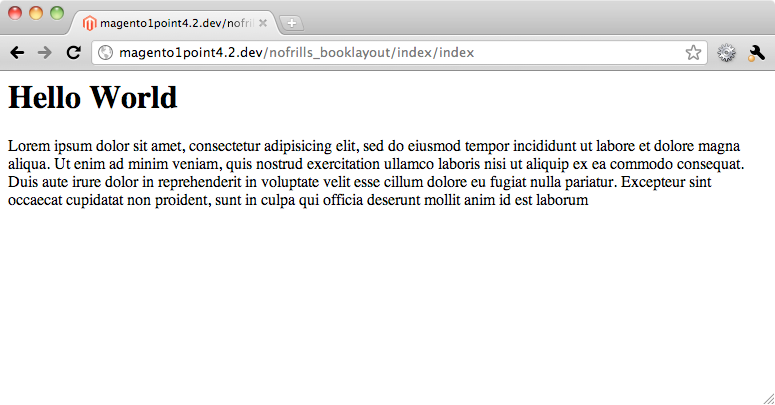
\includegraphics[width=1\textwidth]{images/chapter1/helloworld.png}
\end{center}
\caption{}
%\label{fig:awesome_image}
\end{figure}


Congratulations, you've created your first template block!

\section{Nesting Blocks}

Let's go back to our Layout definition

\begin{quote}
A Layout is a collection of blocks in a tree structure
\end{quote}

We've defined, very basically, what a block is, but what do we mean by "in a tree structure"?

Magento blocks are sort of like HTML nodes.  For example, here

\begin{lstlisting}
<p>
    <span>Lorem</span>
</p>

\end{lstlisting}


The \footnotesize\texttt{\textless p\textgreater } \normalsize  tag is the parent node, and the \footnotesize\texttt{\textless span\textgreater } \normalsize  is the child node.  All blocks share a similar relationship.  Oversimplifying things a bit, this sort of parent/child relationship is known as a "Tree" in computer science circles.

Let's consider our previous template block.  Alter the phtml file so it contains the following

\begin{lstlisting}
<?php #File: app/design/frontend/default/default/template/helloworld.phtml  ?>
<h1>Hello World</h1>
<p>
    <?php echo $this->getChildHtml('the_first'); ?>
</p>
<p>
The second paragraph is hard-coded.
</p>

\end{lstlisting}


There's a few new concepts to cover here.  First, you'll notice we've dropped into PHP code

\begin{lstlisting}
<?php $this->getChildHtml('the_first'); ?>

\end{lstlisting}


You may be wondering what \footnotesize\texttt{\$this} \normalsize  is a reference to.  If you'll remember back to our definition of a template block, we said that each template block object has a phtml template file.  So, when you refer to \footnotesize\texttt{\$this} \normalsize  within a phtml template, you're referring to the template's  block object.  If that's a little fuzzy future examples below should clear things up.

Next, we have the \footnotesize\texttt{getChildHtml} \normalsize  method.  This method will fetch a child block, and call its \footnotesize\texttt{toHtml} \normalsize  method.  This allows you to structure blocks and templates in a logical way. So, with the above code in our template, let's reload the page, (see \emph{Figure 1.3})

\begin{figure}[htb]
\begin{center}
\leavevmode
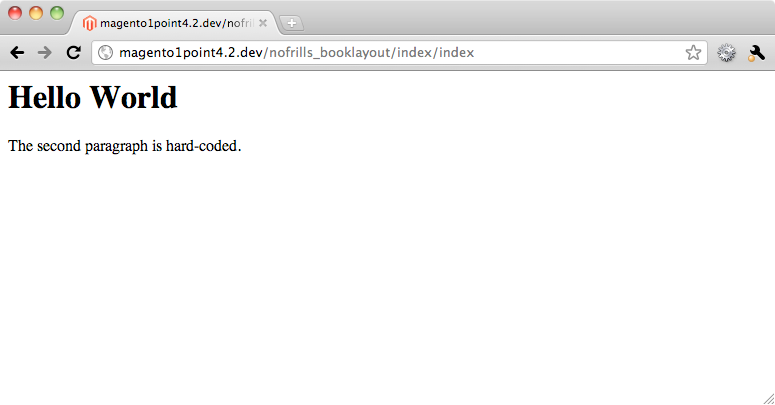
\includegraphics[width=1\textwidth]{images/chapter1/nofirst.png}
\end{center}
\caption{}
%\label{fig:awesome_image}
\end{figure}


Our second hard-coded paragraph rendered, but nothing happened with our call to \footnotesize\texttt{getChildHtml}\normalsize.  That's because we failed to add a child.  Let's change our controller action so it matches the following.

\begin{lstlisting}
public function indexAction()
{
    $paragraph_block = new Mage_Core_Block_Text();
    $paragraph_block->setText('One paragraph to rule them all.');


    $main_block = new Mage_Core_Block_Template();
    $main_block->setTemplate('helloworld.phtml');

    $main_block->setChild('the_first',$paragraph_block);
    echo $main_block->toHtml();
}

\end{lstlisting}


We'll dissect this chunk by chunk.  First, we have the following

\begin{lstlisting}
$paragraph_block = new Mage_Core_Block_Text();
$paragraph_block->setText('One paragraph to rule them all.');

\end{lstlisting}


Here we've created a simple text block.  We've set its text so that when the block is rendered, it will output the sentence \emph{One paragraph to rule them all.}.  Then, as we did before,

\begin{lstlisting}
$main_block = new Mage_Core_Block_Template();
$main_block->setTemplate('helloworld.phtml');

\end{lstlisting}


we define a template block, and point it toward our hello world template.  Finally (and here's the key)

\begin{lstlisting}
$main_block->setChild('the_first',$paragraph_block);

\end{lstlisting}


Here we call a method we haven't see before, called \footnotesize\texttt{setChild}\normalsize.  Here we're telling Magento that the \footnotesize\texttt{\$paragraph\_block} \normalsize  is a child of the \footnotesize\texttt{\$main\_block}\normalsize.  We've also given that block a name (or alias) of \footnotesize\texttt{the\_first}\normalsize.  This name is how we'll refer to the block later, and what we'll pass into our call to \footnotesize\texttt{getChildHtml} \normalsize

\begin{lstlisting}
<?php echo $this->getChildHtml('the_first'); ?>

\end{lstlisting}


Expressed as a generic XML tree, the relationship between blocks might look like

\begin{lstlisting}
<main_block>
    <paragraph_block name="the_first"></paragraph_block>
</main_block>

\end{lstlisting}


Or maybe (getting a bit ahead of ourselves)

\begin{lstlisting}
<block type="core/template" name="root" template="helloworld.phtml">
    <block type="core/text" name="the_first">
        <action name="setText">
            <text>One paragraph to rule them all</text>
        </action>
    </block>
</block>

\end{lstlisting}


A block may have an unlimited number of children, and because we're dealing with PHP 5 objects, changes made to the block after it has been appended will carry through to the final rendered object.  Try the following code

\begin{lstlisting}
public function indexAction()
{
    $block_1 = new Mage_Core_Block_Text();
    $block_1->setText('Original Text');

    $block_2 = new Mage_Core_Block_Text();
    $block_2->setText('The second sentence.');

    $main_block = new Mage_Core_Block_Template();
    $main_block->setTemplate('helloworld.phtml');

    $main_block->setChild('the_first'   ,$block_1);
    $main_block->setChild('the_second'  ,$block_2);

    $block_1->setText('Wait, I want this text instead.');
    echo $main_block->toHtml();
}

\end{lstlisting}


With the following template changes

\begin{lstlisting}
<?php #File: app/design/frontend/default/default/template/helloworld.phtml  ?>
<h1>Hello World</h1>
<p>
    <?php echo $this->getChildHtml('the_first'); ?>
    <?php echo $this->getChildHtml('the_second'); ?>
</p>
<p>
The second paragraph is hard-coded.
</p>

\end{lstlisting}


You should now see output something like

\begin{lstlisting}
Hello World

Wait, I want this text instead.  The second sentence.

The second paragraph is hard-coded.

\end{lstlisting}


One final trick with rendering child blocks.  If you don't provide \footnotesize\texttt{getChildHtml} \normalsize  with the name of a block, \textbf{all child blocks} will be rendered.  That means the following template will give us the same result as the one above

\begin{lstlisting}
<?php #File: app/design/frontend/default/default/template/helloworld.phtml  ?>
<h1>Hello World</h1>
<p>
    <?php echo $this->getChildHtml(); ?>
</p>
<p>
The second paragraph is hard-coded.
</p>

\end{lstlisting}


\section{Advanced Block Functionality}

There's a few more bits of block functionality we should cover before moving on.

The first thing we'll cover is creating your own block classes.  There will be times where you want a block with some custom programmatic functionality.  While it may be tempting to use a standard template block and then include all your logic in the phtml template, the preferred way of doing this is to create a Magento module for adding your own code to the system, and then adding your own block classes that extend the existing classes.

We're not going to cover creating a new module here, although if you're interested in learning the basics then checkout Appendix C.  Instead, we'll have you create your custom block in the \footnotesize\texttt{NoFrills\_Booklayout} \normalsize  module.

So, we just spent a lot of effort to create a hello world block.  Let's take what we've done so far, and create a hello world block.  The first thing we'll want to do is create a new class file at the following location, with the following contents

\begin{lstlisting}
#File: app/code/local/Nofrills/Booklayout/Block/Helloworld.php
<?php
class Nofrills_Booklayout_Block_Helloworld extends Mage_Core_Block_Template
{
}

\end{lstlisting}


And then add the following code to the specific controller action, and load its corresponding URL in your browser

\begin{lstlisting}
#http://magento.example.com/nofrills_booklayout/index/helloblock
public function helloblockAction()
{
    $block_1 = new Mage_Core_Block_Text();
    $block_1->setText('The first sentence. ');

    $block_2 = new Mage_Core_Block_Text();
    $block_2->setText('The second sentence. ');

    $main_block = new Nofrills_Booklayout_Block_Helloworld();
    $main_block->setTemplate('helloworld.phtml');

    $main_block->setChild('the_first',$block_1);
    $main_block->setChild('the_second',$block_2);

    echo $main_block->toHtml();
}

\end{lstlisting}


When you load the page in your browser, you should see your \footnotesize\texttt{helloworld.phtml} \normalsize  template rendered the same as before.

What we've done is create a new block named \footnotesize\texttt{Nofrills\_Booklayout\_Block\_Helloworld}\normalsize. This class extends \footnotesize\texttt{Mage\_Core\_Block\_Template}\normalsize, which means it automatically gains the same functionality as a standard template block.

Next, let's add the following method to our new class,

\begin{lstlisting}
class Nofrills_Booklayout_Block_Helloworld extends Mage_Core_Block_Template
{
    public function _construct()
    {
        $this->setTemplate('helloworld.phtml');
        return parent::_construct();
    }
}

\end{lstlisting}


and remove the \footnotesize\texttt{setTemplate} \normalsize  class in our controller.

\begin{lstlisting}
public function helloblockAction()
{
    $block_1 = new Mage_Core_Block_Text();
    $block_1->setText('The first sentence. ');

    $block_2 = new Mage_Core_Block_Text();
    $block_2->setText('The second sentence. ');

    $main_block = new Nofrills_Booklayout_Block_Helloworld();
    // $main_block->setTemplate('helloworld.phtml');

    $main_block->setChild('the_first',$block_1);
    $main_block->setChild('the_second',$block_2);

    echo $main_block->toHtml();
}

\end{lstlisting}


A page refresh should result in the same exact page.

Every block class can define an optional "pseudo-constructor".  This is a method that's called whenever a new block of this type is created, but that is separate from PHP's standard constructor.  What we've done is ensure that our block \textbf{always} has a template set.

\begin{lstlisting}
    public function _construct()
    {
        $this->setTemplate('helloworld.phtml');
        return parent::_construct();
    }

\end{lstlisting}


There's a few  other special methods you can define in a block class.  The first that we're interested in is \footnotesize\texttt{\_beforeToHtml}\normalsize.  When we call \footnotesize\texttt{toHtml} \normalsize  on our block, this method is called immediately before the block content is rendered.  There's also a corresponding \footnotesize\texttt{\_afterToHtml(\$html)} \normalsize  method which is called after a block is rendered, and is passed the completed HTML string.  We're going to use the \footnotesize\texttt{\_beforeToHtml} \normalsize  method to automatically add our two child blocks, making everything self contained.

\begin{lstlisting}
class Nofrills_Booklayout_Block_Helloworld extends Mage_Core_Block_Template
{
    public function _construct()
    {
        $this->setTemplate('helloworld.phtml');
        return parent::_construct();
    }

    public function _beforeToHtml()
    {
        $block_1 = new Mage_Core_Block_Text();
        $block_1->setText('The first sentence. ');
        $this->setChild('the_first', $block_1);

        $block_2 = new Mage_Core_Block_Text();
        $block_2->setText('The second sentence. ');
        $this->setChild('the_second', $block_2);
    }
}

\end{lstlisting}


This will let us remove the extraneous code from our controller

\begin{lstlisting}
public function helloblockAction()
{
    $main_block = new Nofrills_Booklayout_Block_Helloworld();
    echo $main_block->toHtml();
}

\end{lstlisting}


Again, a page refresh should result in the exact same page.  We've gone from having to manually create our hello world block with 10 or so lines of code to completely encapsulating its functionality and output in 2 lines. This is a pattern you'll see over and over again in Magento.

\section{Block Methods}

The other thing we want to cover is calling, and adding, custom methods to your phtml templates.   Go to your helloworld.phtml file and change the title line so it matches the following.

\begin{lstlisting}
<!-- <h1>Hello World</h1> -->
<h1><?php echo $this->fetchTitle(); ?></h1>

\end{lstlisting}


If you reload your page with this in place, you'll get the following error

\begin{lstlisting}
Invalid method Nofrills_Booklayout_Block_Helloworld::fetchTitle(Array
(
)
)

\end{lstlisting}


As previously mentioned, if you use the \footnotesize\texttt{\$this} \normalsize  keyword in your template, you're referring to a template's parent block object.  Let's add a method that returns the page title

\begin{lstlisting}
class Nofrills_Booklayout_Block_Helloworld extends Mage_Core_Block_Template
{
    public function _construct()
    {
        $this->setTemplate('helloworld.phtml');
        return parent::_construct();
    }

    public function _beforeToHtml()
    {
        $block_1 = new Mage_Core_Block_Text();
        $block_1->setText('The first sentence. ');
        $this->setChild('the_first', $block_1);

        $block_2 = new Mage_Core_Block_Text();
        $block_2->setText('The second sentence. ');
        $this->setChild('the_second', $block_2);
    }

    public function fetchTitle()
    {
        return 'Hello Fancy World';
    }
}

\end{lstlisting}


Reload the page with the above \footnotesize\texttt{Nofrills\_Booklayout\_Block\_Helloworld} \normalsize  in place, and you'll see your page with its new title.

This is the preferred way to create templates with dynamic data in Magento.  Your \footnotesize\texttt{phtml} \normalsize  file should contain

\begin{enumerate}
\item HTML/CSS/Javascript code
\item Calls to echo
\item Looping and control structures
\item Calls to block methods
\end{enumerate}


Any PHP more complicated than the above should be put in block methods. This includes calls to Magento models to read back data which was saved in the controller layer.

\section{Enter the Layout}

Coming back again to our definition of a Layout

\begin{quote}
A Layout is a collection of blocks in a tree structure
\end{quote}

We now know what a block is and what a block can do.  We understand how blocks are organized in a tree like structure.  The only thing that leaves us to cover is the layout object itself.

A layout object, (instantiated from a \footnotesize\texttt{Mage\_Core\_Model\_Layout} \normalsize  class)

\begin{itemize}
\item Is a wrapper object for interacting with your blocks.
\item Provides helper methods for creating blocks
\item Allows you to designate which block should start the rendering for a page
\item Provides a mechanism for loading complex layouts described by XML files
\end{itemize}


Let's take a look at some layout examples.  Add the following action to our controller

\begin{lstlisting}
#http://magento.example.com/nofrills_booklayout/index/layout
public function layoutAction()
{
    $layout = Mage::getSingleton('core/layout');
    $block = $layout->createBlock('core/template','root');
    $block->setTemplate('helloworld-2.phtml');
    echo $block->toHtml();
}

\end{lstlisting}


Next, create a file named \footnotesize\texttt{helloworld-2.phtml} \normalsize  that's in the same location as your \footnotesize\texttt{helloworld.phtml} \normalsize  template.

\begin{lstlisting}
<?php #File: app/design/frontend/default/default/template/helloworld-2.phtml  ?>
<h1><?php //echo $this->fetchTitle(); ?></h1>
<h1>Hello World 2</h1>
<p>
    <?php echo $this->getChildHtml(); ?>
</p>
<p>
The second paragraph is hard-coded.
</p>

\end{lstlisting}


Load your page and you'll see the second hello world template rendered in your browser, without any output for \footnotesize\texttt{getChildHtml} \normalsize  (as we didn't add any child nodes).

There's a lot new going on here, so let's cover things line by line.

\begin{lstlisting}
$layout = Mage::getSingleton('core/layout');

\end{lstlisting}


This instantiates your layout object as a singleton model (see below). The string \footnotesize\texttt{core/layout} \normalsize  is known as a class alias.  It's beyond the scope of this book to go fully into what class aliases are used for (see Appendix B: Class Alias for a better description), but from a high level; when creating a Magento model, a class alias is used as a shortcut notation for a full class name.  It can be translated into a class name by the following set of transformations

\begin{lstlisting}
Core Layout             //adding a space at the slash, and capitalizing
Core Model Layout       //Add the word Model in between
Mage Core Model Layout  //Add the word Mage before
Mage_Core_Model_Layout  //underscore the spaces

\end{lstlisting}


This is a bit of an over simplification, but for now when you see something like

\begin{lstlisting}
$o = Mage::getModel('foo/bar');
$o = Mage::getSingleton('foo/bar');

\end{lstlisting}


just substitue

\begin{lstlisting}
$o = new Mage_Foo_Model_Bar();

\end{lstlisting}


in your mind.

\subsection{What's a Singleton!?}

A singleton is a fancy object oriented programming term for an object that may only be instantiated once.  The first time you instantiate it, a new object will be created.  However, if you attempt to instantiate the object again, rather than create a new object, the originally created object will be returned.

A singleton is used when you only want to create a single instance of any type of object.  Magento assumes you'll only want to render \textbf{one} HTML page per request (probably a safe assumption), and by using a singleton it's ensured you're always getting the same layout object.

If all that went over your head don't worry.  All you need to know is whenever you want to get a reference to your layout object, use

\begin{lstlisting}
$layout = Mage::getSingleton('core/layout');

\end{lstlisting}


\section{Back to the Code}

Next up we have the line

\begin{lstlisting}
$block = $layout->createBlock('core/template','root');

\end{lstlisting}


This line creates a \footnotesize\texttt{Mage\_Core\_Template\_Block} \normalsize  object named \footnotesize\texttt{root} \normalsize  (we'll get to the why of "\footnotesize\texttt{root} \normalsize " in a bit) by calling the \footnotesize\texttt{createBlock} \normalsize  method on our newly instantiated layout object.

Again, in place of a class name, we have the \footnotesize\texttt{core/template} \normalsize  class alias.  Because we're using the class alias to instantiate a \textbf{block}, this translates to

\begin{lstlisting}
Mage_Core_Block_Template

\end{lstlisting}


Again, check Appendix B if you're interested in how class aliases are resolved.  Whenever we use a class alias for the remainder of this book, we'll let you know the real PHP class.

Everything else from here on out should look familiar.  The following

\begin{lstlisting}
$block->setTemplate('helloworld-2.phtml');
echo $block->toHtml();

\end{lstlisting}


sets our block template, and renders the block using its \footnotesize\texttt{toHtml} \normalsize  method.  Let's use a class alias to instantiate our custom block from the previous examples

\begin{lstlisting}
//class alias 'nofrills_booklayout/helloworld' is translated into
//the class name Nofrills_Booklayout_Block_Helloworld
public function layoutAction()
{
    $layout = Mage::getSingleton('core/layout');
    $block = $layout->createBlock('nofrills_booklayout/helloworld','root');
    echo $block->toHtml();
}

\end{lstlisting}


Reload the page, you should see our original block.

\section{Who's the Leader}

Give our next example a try

\begin{lstlisting}
public function layoutAction()
{
    $layout = Mage::getSingleton('core/layout');
    $block = $layout->createBlock('nofrills_booklayout/helloworld','root');

    $layout->addOutputBlock('root');
    $layout->setDirectOutput(true);
    $layout->getOutput();
}

\end{lstlisting}


Refresh the page, and you should see the same output as your did before.

What we've done here is replace our call to the block's \footnotesize\texttt{toHtml} \normalsize  with the following

\begin{lstlisting}
$layout->addOutputBlock('root');
$layout->setDirectOutput(true);
$layout->getOutput();

\end{lstlisting}


The call to \footnotesize\texttt{addOutputBlock} \normalsize  tells our layout block that \textbf{this} is the block that should start the page rendering process.  Following that is a call to \footnotesize\texttt{getOutput}\normalsize,  which is the call that actually \textbf{starts} the page rendering process.  Every time you use \footnotesize\texttt{createBlock} \normalsize  to create an object, the Layout object will know about that block.  That's why we gave it a name earlier.

The call to \footnotesize\texttt{setDirectOutput} \normalsize  is us telling the Layout object that it should just automatically \footnotesize\texttt{echo} \normalsize  out the results of the page.   If we wanted to capture the results as a string instead, we'd just use

\begin{lstlisting}
$layout->addOutputBlock('root');
$layout->setDirectOutput(false);
$output = $layout->getOutput();

\end{lstlisting}


\section{Method Chaining}

Now's probably a good time to mention a PHP feature that Magento makes extensive use of called method chaining.  Let's replace our code from above with the following.

\begin{lstlisting}
public function layoutAction()
{
    $layout = Mage::getSingleton('core/layout');
    $block = $layout->createBlock('nofrills_booklayout/helloworld','root');
    echo $layout->addOutputBlock('root')->setDirectOutput(false)->getOutput();
}

\end{lstlisting}


You'll notice that we've trimmed a few lines from the code, but that we're using a funky syntax in that last line.

\begin{lstlisting}
echo $layout->addOutputBlock('root')->setDirectOutput(false)->getOutput();

\end{lstlisting}


This is method chaining. It's not a Magento feature per se, but it's a feature of PHP that's become much more popular as applications start leveraging PHP 5 OOP capabilities.

If a call to a method returns an object, PHP lets you chain a another method call on the end for brevity. This can be repeated as long as each method call returns an object.  The above is equivalent to the following

\begin{lstlisting}
$block = $layout->addOutputBlock('root');
$block->setDirectOutput(false);
echo $block->getOutput();

\end{lstlisting}


You'll also see chaining syntax that spans multiple lines

\begin{lstlisting}
$layout->addOutputBlock('root')
->setDirectOutput(false)
->getOutput();

\end{lstlisting}


Again, this isn't anything that's specific to Magento.  It's just a pattern that's becoming more popular with PHP developers as PHP 5 style objects are used more and more.  Magento \textbf{enables} this syntax by having most of its set, create, and add methods return an appropriate object. You're not required to use it, but get used to seeing it if you spend any time with core or community modules

\section{A Full Page Layout}

From here on out we're going to start using a special block we've created in the Nofrills module you installed.  It's called

\begin{lstlisting}
nofrills_booklayout/template
Nofrills_Booklayout_Block_Template

\end{lstlisting}


The block is identical to the Core template block, with one exception.

\begin{lstlisting}
public function fetchView($fileName)
{
    //ignores file name, just uses a simple include with template name
    $this->setScriptPath(
        Mage::getModuleDir('', 'Nofrills_Booklayout') .
        DS .
        'design'
    );
    return parent::fetchView($this->getTemplate());
}

\end{lstlisting}


We've overridden the \footnotesize\texttt{fetchView} \normalsize  function in our template with the code above.  What this does is move the base folder for templates from

\begin{lstlisting}
app/design

\end{lstlisting}


to a folder in our local module hierarchy.

\begin{lstlisting}
app/code/local/Nofrills/Booklayout/design

\end{lstlisting}


This has allowed us to package our template files in the same folder as our PHP files, and save you from a lot of copy/paste

Let's open up the URL that corresponds to the Layoutdemo controller

\begin{lstlisting}
#URL:   http://magento.example.com/nofrills_booklayout/layoutdemo
#File:  app/code/local/Nofrills/Booklayout/controllers/LayoutdemoController.php

\end{lstlisting}


You should see a browser screen that looks like \emph{Figure 1.4}

\begin{figure}[htb]
\begin{center}
\leavevmode
\includegraphics[width=1\textwidth]{images/chapter1/twocities.png}
\end{center}
\caption{}
%\label{fig:awesome_image}
\end{figure}


If you view the source of this page, you'll see we have a full (if very basic) HTML page structure.  Let's take a look at the code we used to create the layout and blocks necessary to pull this off.

\begin{lstlisting}
#File: app/cod/local/Nofrills/Booklayout/controllers/LayoutdemoController.php
class Nofrills_Booklayout_LayoutdemoController
extends Mage_Core_Controller_Front_Action
{
    public function _initLayout()
    {
        $layout         = Mage::getSingleton('core/layout');
        $layout->addOutputBlock('root');

        $additional_head = $layout->createBlock(
        'nofrills_booklayout/template','additional_head')
        ->setTemplate('simple-page/head.phtml');


        $sidebar = $layout->createBlock('nofrills_booklayout/template','sidebar')
        ->setTemplate('simple-page/sidebar.phtml');

        $content = $layout->createBlock('core/text_list', 'content');

        $root    = $layout->createBlock('nofrills_booklayout/template','root')
        ->setTemplate('simple-page/2col.phtml')
        ->insert($additional_head)
        ->insert($sidebar)
        ->insert($content);

        return $layout;
    }

    public function indexAction()
    {
        $layout = $this->_initLayout();

        $text = $layout->createBlock('core/text','words');
        $text->setText('It was the best of times, it was the BLURST?! of times?');

        $content = $layout->getBlock('content');
        $content->insert($text);

        $layout->setDirectOutput(true);
        $layout->getOutput();

        exit;
    }
}

\end{lstlisting}


Again, we have some new concepts we'll need to cover here.

\section{Initializing the Layout and Setting Content}

The first thing you'll notice is the \footnotesize\texttt{\_initLayout} \normalsize  layout method.  We're using this controller method to setup a base layout object that has common components (like navigation, some \footnotesize\texttt{\textless head\textgreater } \normalsize  HTML, etc.) defined.   This allows many different controller methods to share the same basic layout, without us having to rewrite the setup code every time.  Instead, all each action would need to do is call

\begin{lstlisting}
$layout = $this->_initLayout();

\end{lstlisting}


and a base/shared layout would already be created.

\section{Insert vs. Set}

You also probably noticed we're not using the \footnotesize\texttt{setChild} \normalsize  method to add blocks to our layout.  Instead, we're using the \footnotesize\texttt{insert} \normalsize  to add child blocks to other blocks.

\begin{lstlisting}
->insert($additional_head)

\end{lstlisting}


The \footnotesize\texttt{insert} \normalsize  method is the preferred method for adding child blocks to an existing block.    There's a bit of redundancy in the \footnotesize\texttt{setChild} \normalsize  method, as it requires you to pass in a name for your block.

\begin{lstlisting}
$block->setChild('block_name', $block);

\end{lstlisting}


However, the \footnotesize\texttt{insert} \normalsize  method will automatically use the name you set when you created it (the following code created a block named "sidebar")

\begin{lstlisting}
$layout->createBlock('nofrills_booklayout/template','sidebar');

\end{lstlisting}


There are a few other problems with using \footnotesize\texttt{setChild} \normalsize  in a public context; as of CE 1.4.2 it still doesn't add blocks to the internal \footnotesize\texttt{\_sortedBlocks} \normalsize  array, which will cause problems down the road, (see Chapter 5 for more information).

Stick with \footnotesize\texttt{insert} \normalsize  method and you'll be a happy camper.

\section{Getting a Reference and Text List}

So, the \footnotesize\texttt{\_initLayout} \normalsize  method serves as a central location for instantiating a base layout object.  Templates are set, and a complete layout object with an empty "content" node is returned.  We'll want to turn our attention to the following code.

\begin{lstlisting}
$text = $layout->createBlock('core/text','words');
$text->setText('It was the best of times, it was the BLURST?! of times?');

$content = $layout->getBlock('content');
$content->insert($text);

\end{lstlisting}


The first two lines should look familiar.  We're creating a simple \footnotesize\texttt{core/text (Mage\_Core\_Block\_Text)} \normalsize  block that looks like it was written by an infinite number of monkeys - 1.  The next set of lines is far more interesting.  The \footnotesize\texttt{getBlock} \normalsize  method allows you to re-obtain a reference to any block that's been added to the layout (including those added using \footnotesize\texttt{createBlock}\normalsize).

What this code does is get a reference to the content block that was added in \footnotesize\texttt{\_initLayout}\normalsize, and then \textbf{add} our new content block to it.  The \footnotesize\texttt{getBlock} \normalsize  method is what allows us to centralize the creation of a general layout, and then customize it further for any specific action's needs.

Let's look back up at the creation of our block named content.

\begin{lstlisting}
$content = $layout->createBlock('core/text_list', 'content');

\end{lstlisting}


You'll notice we used the class alias \footnotesize\texttt{core/text\_list} \normalsize  here, which corresponds to the class Mage\_Core\_Block\_Text\_List.  Text list blocks have a slightly deceptive name, as you don't set their text.  Instead, what a \footnotesize\texttt{core/text\_list} \normalsize  block does is \textbf{automatically} render \textbf{all} child blocks that have been added to it.

This feature of the \footnotesize\texttt{core/text\_list} \normalsize  block is what allows us to add a block named content and just start \footnotesize\texttt{insert}\normalsize ing blocks into it.  Any block we add will be automatically rendered.

\section{A Recap and a Dilema}

Look back one last time at our definition of a Layout

\begin{quote}
A Layout is a collection of blocks in a tree structure
\end{quote}

We appear to have covered everything a layout is.  We know what a block is, we know how to create a nested structure of blocks, and we now understand how the Layout object provides command and control for the entire show.  We've also seen how a generic layout can be built, and then added to depending on our needs.

However, by answering these questions, we've created a new one.  \textbf{How} should Magento create the layouts needed for each page?  Consider our example code above where we abstracted the creation of the Layout object to a \footnotesize\texttt{\_initLayout} \normalsize  method. This made sense for the tutorials, but Magento core code contains over 180 controllers.  If we put layout instantiation in each controller, that means anytime the core team wanted to make a change to the base layout we'd need to update over 180 files.  These different \footnotesize\texttt{\_initLayout} \normalsize  functions would inevitably start to differ in slight ways, eventually causing incompatibility.

The next choice would be to create a separate, centralized, master Layout object for the base layout. Core system programmers could then get a reference to the object, and add to it as need be.  This solves some problems, but creates a situation where we're either relying on system programmers whenever designers need to change something, or letting designers into core system code to change highly abstracted PHP code they may not understand.  While services based agencies have long used designer/coders and coder/designers, this metaphor hasn't penetrated as deeply in the computer science world, which prefers a layer of separation between the two worlds.

Magento's solution to this situation was to create a system where designers could \textbf{configure} what layout they wanted for any particular URL request in Magento.  This is the Layout XML system that many of you are already familiar with, and the system that we'll be diving into in our next chapter.

\emph{Visit http://www.pulsestorm.net/nofrills-layout-chapter-one to join the discussion online.}
\chapter{XML Page Layout Files}
The core problem the Magento Layout XML system sets out to solves is

\begin{quote}
How do we allow designers and theme developers to configure a layout, but still offer them full control over the HTML output if they need/want it
\end{quote}

So why XML? XML gets used for a lot of things.  If you've been doing web development for a while you probably think of XML as a generic document format. While that's \textbf{one} of the things XML can be used for, software engineers and computer scientists have other uses for it.

The Magento XML Layout format is less a document format, and more a mini-programming language.  The Magento core team created a special format of XML files that fully describes the process of creating blocks programmatically that was described in the previous chapter.  There is no public schema or DTD for this dialect of XML, but don't worry, by the time we're through with this chapter you'll have the format down cold.

The Magento Layout XML System is made up of multiple independent pieces.  It may seem like some of what we're doing is more of a hassle than just using PHP to create our blocks.  However, once you've seen all the pieces, and how those pieces fit together, the advantages of the system should be apparent.

All of which is a fancy way of saying, "Hang in There".  This is new, this is different than what you're used to, but it's no harder than any other web development you've learned before.

Finally, while not 100\% necessary, the content of this chapter assumes you've been through Chapter 1.  Even if you're a master at creating blocks programmatically, you may want to skim through the previous chapter before venturing on.

\section{Hello World in XML}

We'll be working in \footnotesize\texttt{UpdateController.php} \normalsize  in this chapter, which may be accessed at the following URL/file

\begin{lstlisting}
http://magento.example.com/nofrills_booklayout/update
app/code/local/Nofrills/Booklayout/controllers/UpdateController.php

\end{lstlisting}


The first type of XML tree Magento uses is called the Page Layout.  We say tree instead of file, as the Page Layout XML is normally generated on the fly.  We're going to create a few Page Layouts manually to get an idea of how they work.

In the previous chapter, we created a Hello World block with a class alias of \footnotesize\texttt{nofrills\_booklayout/helloworld} \normalsize  (corresponding to the class \footnotesize\texttt{Nofrills\_Booklayout\_Block\_Helloworld}\normalsize).  Let's start by creating a Page Layout that uses this block.

First, here's the XML we'll use

\begin{lstlisting}
<layout>
    <block type="nofrills_booklayout/helloworld" name="root" output="toHtml" />
</layout>

\end{lstlisting}


We have an XML node with a root node named layout.  Within the root node is a single block node with three attributes; type, name, and output.

The \textbf{type} attribute is where we specify the class alias of the block we'd like to instantiate.  The \footnotesize\texttt{name} \normalsize  attribute allows us to set a name for the block which can be used later to get a reference.  The \footnotesize\texttt{output="toHtml"} \normalsize  attribute/value pair tells the layout system that \textbf{this} is the block which should start output.

The Page Layout XML above is roughly equivalent to the following PHP code

\begin{lstlisting}
$layout = new Mage::getSingleton('core/layout');
$layout->createBlock('nofrills_booklayout/helloworld','root');
$layout->addOutputBlock('root','toHtml')

\end{lstlisting}


You'll notice we've passed in a second parameter ('\footnotesize\texttt{toHtml}\normalsize') to the \footnotesize\texttt{addOutputBlock} \normalsize  method.  This is an optional parameter that tells the layout object \textbf{which method} on the output block should be be used to kick off output.  If you look at its definition, it normally defaults to \footnotesize\texttt{toHtml} \normalsize

\begin{lstlisting}
public function addOutputBlock($blockName, $method='toHtml')
{
    //$this->_output[] = array($blockName, $method);
    $this->_output[$blockName] = array($blockName, $method);
    return $this;
}

\end{lstlisting}


In practice you'll never set this optional parameter, but we're including it here to make it more clear what the output attribute in the XML node above is doing

\section{An Interesting use of the Word Simple}

Let's load our XML into the layout object and use it to generate our output.  Edit the \footnotesize\texttt{indexAction} \normalsize  method in \footnotesize\texttt{UpdateController.php} \normalsize  so it matches the following

\begin{lstlisting}
public function indexAction()
{
    $layout = Mage::getSingleton('core/layout');
    $xml = simplexml_load_string('<layout>
            <block type="nofrills_booklayout/helloworld"
            name="root" output="toHtml" />
        </layout>','Mage_Core_Model_Layout_Element');

    $layout->setXml($xml);
    $layout->generateBlocks();
    echo $layout->setDirectOutput(true)->getOutput();
}

\end{lstlisting}


Load the code above in a browser at

\begin{lstlisting}
http://magento.example.com/nofrills_booklayout/update

\end{lstlisting}


and you should see your Hello World block.

The first thing that may look a little unfamiliar about the code above is the fragment that creates our simple XML object.

\begin{lstlisting}
$xml = simplexml_load_string('<layout>
<block type="nofrills_booklayout/helloworld" name="root" output="toHtml" />
</layout>','Mage_Core_Model_Layout_Element');

\end{lstlisting}


You may have never seen a SimpleXML node created with that second parameter

\begin{lstlisting}
Mage_Core_Model_Layout_Element

\end{lstlisting}


One of SimpleXML's lesser known features is the ability to tell PHP to use a user defined class to represent the nodes.  By default, a SimpleXML node is a object of type \footnotesize\texttt{SimpleXMLElement}\normalsize, which is a PHP built-in.  By using the syntax above, the Magento core code is telling PHP

\begin{quote}
Make our simple XML nodes objects of type \footnotesize\texttt{Mage\_Core\_Model\_Layout\_Element} \normalsize  instead of type SimpleXMLElement
\end{quote}

If you look at the inheritance chain, you can see that the \footnotesize\texttt{Mage\_Core\_Model\_Layout\_Element} \normalsize  class has \footnotesize\texttt{SimpleXMLElement} \normalsize  as an ancestor.

\begin{lstlisting}
class Mage_Core_Model_Layout_Element extends Varien_Simplexml_Element {...}
class Varien_Simplexml_Element extends SimpleXMLElement {...}

\end{lstlisting}


So, the Magento provided class name extends \footnotesize\texttt{SimpleXMLElement}\normalsize. That means all normal SimpleXML functionality is preserved.

If you tried to use \footnotesize\texttt{setXml} \normalsize  with a normal \footnotesize\texttt{SimpleXMLElement}\normalsize, you'd end up with an error that looks something like this

\begin{lstlisting}
Recoverable Error: Argument 1 passed to Varien_Simplexml_Config::setXml()
must be an instance of Varien_Simplexml_Element, instance of
SimpleXMLElement given

\end{lstlisting}


That's because Magento uses PHP's type hinting features to ensure that a normal SimpleXMLElement based object can't be used.

\begin{lstlisting}
//notice the Varien_Simplexml_Element type hinting
public function setXml(Varien_Simplexml_Element $node)
{
    ...

\end{lstlisting}


This is another example of Magento's object oriented system design. Some of you are probably thinking "\textbf{That's nuts! Why would you want to do this?}"  By providing a custom class here, we gain the ability to add custom methods to any XML node.  For example, if we were using the default SimpleXMLElement node, every time we wanted to grab a block's name attribute we'd need to do something like this

\begin{lstlisting}
    $tagName = (string)$node->getName();
    if ('block'!==$tagName && 'reference'!==$tagName || empty($node['name'])) {
        $name = false;
    }
    $name = (string)$node['name'];

\end{lstlisting}


Using the SimpleXML custom class feature, we can define a method on our class to do this for us

\begin{lstlisting}
public function getBlockName()
{
    $tagName = (string)$this->getName();
    if ('block'!==$tagName && 'reference'!==$tagName || empty($this['name'])) {
        return false;
    }
    return (string)$this['name'];
}

\end{lstlisting}


and then use it wherever we want, resulting in cleaner end-user code which is easier to read and understand

\begin{lstlisting}
$name = $node->getBlockName();

\end{lstlisting}


If you're not convinced, a little paraphrased Tennyson might help you along the way

\begin{quote}
Ours is not to question why/Ours is but to do or die
\end{quote}

\section{Adding the XML, Generating the Blocks}

So, that little foray in lesser known PHP features complete, the next bit it pretty straight forward.  Our Layout object is responsible for managing our  Page Layout XML

\begin{lstlisting}
    $layout = Mage::getSingleton('core/layout');

\end{lstlisting}


Page Layout XML is one of its jobs.  After getting a reference to the Layout object, we set our newly created simple XML object

\begin{lstlisting}
    $layout->setXml($xml);

\end{lstlisting}


Next, we tell the Layout object to use the Page Layout XML to generate the needed block objects

\begin{lstlisting}
    $layout->generateBlocks();

\end{lstlisting}


This doesn't create any output.  When you call the \footnotesize\texttt{generateBlocks} \normalsize  method, it goes through your Page Layout XML and creates all the PHP block objects that are needed to generate your layout.  The Page Layout XML \textbf{configures} which blocks are used as well as the parent/child relationships between those blocks.

It's not until we call

\begin{lstlisting}
    echo $layout->setDirectOutput(true)->getOutput();

\end{lstlisting}


that the \footnotesize\texttt{toHtml} \normalsize  method is called and rendering begins.

\section{Getting a Little More Complex}

Let's take a look at a layout that's a bit more complex.  Create a new action in the \footnotesize\texttt{UpdateController.php} \normalsize  file, and load its corresponding URL

\begin{lstlisting}
#URL: http://magento.example.com/nofrills_booklayout/update/complex
public function complexAction()
{
    $layout = Mage::getSingleton('core/layout');
    $path   = Mage::getModuleDir('', 'Nofrills_Booklayout') . DS .
    'page-layouts' . DS . 'complex.xml';
    $xml = simplexml_load_file($path,
    Mage::getConfig()->getModelClassName('core/layout_element'));
    $layout->setXml($xml);
    $layout->generateBlocks();
    echo $layout->setDirectOutput(true)->getOutput();
}

\end{lstlisting}


Before we get into the Layout XML itself, there's two new things going on here, both related to how we're loading our XML. First,

\begin{lstlisting}
$path   = Mage::getModuleDir('', 'Nofrills_Booklayout') . DS .
'page-layouts' . DS . 'complex.xml';
$xml = simplexml_load_file($path,
Mage::getConfig()->getModelClassName('core/layout_element'));

\end{lstlisting}


you'll notice we're loading our Page Layout XML from a file rather than passing in a string.  This isn't necessary, but will make it easier for us to examine/add-to the XML.

The second thing you'll notice is we've replaced the hard coded XML element class

\begin{lstlisting}
Mage_Core_Model_Layout_Element

\end{lstlisting}


with a call to

\begin{lstlisting}
Mage::getConfig()->getModelClassName('core/layout_element')

\end{lstlisting}


While current versions of Magento use a \footnotesize\texttt{Mage\_Core\_Model\_Layout\_Element}\normalsize, it's possible that a future version may change this.  Because of that, Magento engineers store and read this class name from a config file.  When possible, it's best to follow the same conventions you see in Magento core code to ensure maximum compatibility with future versions.  Again, this is something you won't need to concern yourself with while \textbf{using} the Layout system, rather it's something you'd want to understanding if you're working on extending it.

Alright!  Let's take a look at the layout we just rendered and the XML that created it, (see \emph{Figure 2.1})

\begin{figure}[htb]
\begin{center}
\leavevmode
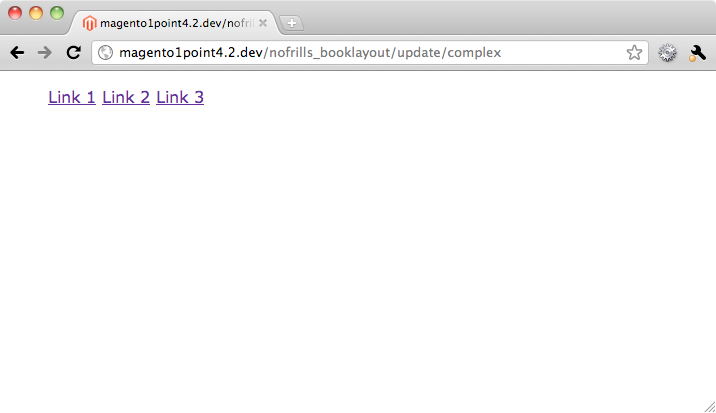
\includegraphics[width=1\textwidth]{images/chapter2/complex.png}
\end{center}
\caption{}
%\label{fig:awesome_image}
\end{figure}


If you look at the \footnotesize\texttt{complex.xml} \normalsize  file (bundled with the Chapter 2 module code),

\begin{lstlisting}
app/code/local/Nofrills/Booklayout/page-layouts/complex.xml

\end{lstlisting}


you'll see the following

\begin{lstlisting}
<layout>
    <block type="nofrills_booklayout/template" name="root"
    template="simple-page/2col.phtml" output="toHtml">
        <block type="nofrills_booklayout/template" name="additional_head"
        template="simple-page/head.phtml" />

        <block type="nofrills_booklayout/template" name="sidebar">
            <action method="setTemplate">
                <template>simple-page/sidebar.phtml</template>
            </action>
        </block>

        <block type="core/text_list" name="content" />

    </block>
</layout>

\end{lstlisting}


Lots of new and interesting things to discuss here.  The first thing you'll notice is that we've added some sub-nodes to our parent block, as well as introduced a new attribute named template.

\begin{lstlisting}
<block type="nofrills_booklayout/template" name="root"
template="simple-page/2col.phtml" output="toHtml">
    ...
</block>

\end{lstlisting}


You'll remember that a \footnotesize\texttt{nofrills\_booklayout/template} \normalsize  block is our version of Magento's \footnotesize\texttt{core/template} \normalsize  block.  When your block is a template block, you can specify which template it should use in the template attribute

\begin{lstlisting}
template="simple-page/2col.phtml"

\end{lstlisting}


When you nest blocks in a Page Layout XML tree, it's the equivalent of using the \footnotesize\texttt{insert} \normalsize  method when you're creating them programmatically.  The node structure of the XML mirrors the parent/child relationships you were previously setting up programmatically.

Depending on how well you're following along (and if you've taken a few days off to digest everything and/or drink heavily), you may be wondering why it's only the top level node that has a \footnotesize\texttt{output} \normalsize  attribute.  How does Magento know how to render the sub-blocks?  The answer, of course, is in your \footnotesize\texttt{simple-page/2col.phtml} \normalsize  template.

\begin{lstlisting}
File: app/code/local/Nofrills/Booklayout/design/simple-page/2col.phtml
<!DOCTYPE html>
<html>
<head>
    <meta charset="utf-8" />
    <title></title>
    <?php echo $this->getChildhtml('additional_head'); ?>
</head>
<body>
    <?php echo $this->getChildhtml('sidebar'); ?>
    <section>
    <?php echo $this->getChildhtml('content'); ?>
    </section>
</body>
</html>

\end{lstlisting}


The phtml template files don't care how their parent blocks have been instantiated, they'll function the same regardless of whether they've been created with PHP code or XML code.  The \footnotesize\texttt{simple-page/2col.phtml} \normalsize  template is still looking for a child block named (in this example) \footnotesize\texttt{additional\_head}\normalsize.  That's why it's important that all your sub block  \footnotesize\texttt{\textless block/\textgreater } \normalsize  elements have names

\begin{lstlisting}
name="additional_head"
name="sidebar"
name="content"

\end{lstlisting}


\section{Action Methods}

Another new node is the \footnotesize\texttt{\textless action/\textgreater } \normalsize  node.  Let's take a look at the sidebar block

\begin{lstlisting}
<block type="nofrills_booklayout/template" name="sidebar">
    <action method="setTemplate">
        <template>simple-page/sidebar.phtml</template>
    </action>
</block>

\end{lstlisting}


Here you'll see we're still using a template block, but we've left off the \footnotesize\texttt{template} \normalsize  attribute.  Instead, we've added a sub-node named \footnotesize\texttt{\textless action/\textgreater }\normalsize.

An \footnotesize\texttt{\textless action/\textgreater } \normalsize  node will allow you to call methods on the block which contains it.  The above node is equivalent to the following PHP code

\begin{lstlisting}
$layout = Mage::getSingleton('core/layout');
$block = $layout->createBlock('nofrills_booklayout/template','sidebar');
$block->setTemplate('simple-page/sidebar.phtml');

\end{lstlisting}


You can call \textbf{any} public method on a block this way, although some methods won't have any meaning when called from XML.  Here we've used it as an alternate method of setting a template, but the Magento core themes are filled with other practical examples.  Consider the \footnotesize\texttt{page/html\_head} \normalsize  blocks (\footnotesize\texttt{Mage\_Core\_Block\_Html\_Head}\normalsize).  They contain a number of methods for adding CSS and Javascript files to your page

\begin{lstlisting}
<action method="addCss"><stylesheet>css/styles.css</stylesheet></action>
<action method="addJs"><script>lib/ccard.js</script></action>

\end{lstlisting}


We'll cover the \footnotesize\texttt{\textless action/\textgreater } \normalsize  node in greater depth later on in Chapter 5.  You also may be interested in Appendix D, which contains a full list, in XML format, of what actions may be called from what blocks.

\section{References and the Importance of text\_lists}

To review: We've rendered out our blank page template again, but this time with XML.  Let's add some content to it.  Edit your \footnotesize\texttt{complexAction} \normalsize  method so it matches the following

\begin{lstlisting}
public function complexAction()
{
    $layout = Mage::getSingleton('core/layout');
    $path   = Mage::getModuleDir('', 'Nofrills_Booklayout') . DS .
    'page-layouts' . DS . 'complex.xml';
    $xml = simplexml_load_file($path,
    Mage::getConfig()->getModelClassName('core/layout_element'));
    $layout->setXml($xml);

    $text = $layout->createBlock('core/text','foxxy')
    ->setText("The quick brown fox jumped over the lazy dog.");

    $layout->generateBlocks();
    $layout->getBlock('content')->insert($text);

    echo $layout->setDirectOutput(true)->getOutput();
}

\end{lstlisting}


Just as we were able to in the previous chapter, we obtained a reference to the \footnotesize\texttt{content} \normalsize  block, and inserted a new text block for the page.  It's important to note that we couldn't do this \textbf{before} we'd called  \footnotesize\texttt{generateBlocks}\normalsize. If we tried to, we'd get an error along the lines of

\begin{lstlisting}
Call to a member function insert() on a non-object

\end{lstlisting}


because we can't get a reference to a block before it's been created.  Reload the page and you'll see our new content, (see \emph{Figure 2.2})

\begin{figure}[htb]
\begin{center}
\leavevmode
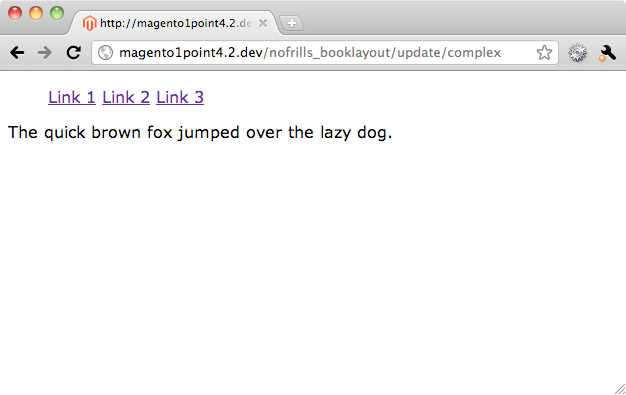
\includegraphics[width=1\textwidth]{images/chapter2/with-content.png}
\end{center}
\caption{}
%\label{fig:awesome_image}
\end{figure}


Of course, now we're back to adding things to the layout via PHP.  Wouldn't it be nice if there was a way to get references to blocks via the Page Layout XML? As you might have guessed by our overtly rhetorical tone, The Page Layout XML offers just such capabilities.  At the top level of \footnotesize\texttt{complex.xml} \normalsize  add the node named \footnotesize\texttt{\textless reference/\textgreater } \normalsize  below and give your page a refresh.

\begin{lstlisting}
<layout>
    <block type="nofrills_booklayout/template" name="root"
    template="simple-page/2col.phtml" output="toHtml">

        <block type="nofrills_booklayout/template" name="additional_head"
        template="simple-page/head.phtml" />

        <block type="nofrills_booklayout/template" name="sidebar">
            <action method="setTemplate">
                <template>simple-page/sidebar.phtml</template>
            </action>
        </block>

        <block type="core/text_list" name="content" />

    </block>


    <reference name="content">
        <block type="core/text" name="goodbye">
            <action method="setText">
                <text> The lazy dog was only faking it. </text>
            </action>
        </block>

    </reference>
</layout>

\end{lstlisting}


Voila!  Another node added to content.

The \footnotesize\texttt{\textless reference/\textgreater } \normalsize  tag is the other tag that's valid at the top level of a Page Layout XML \footnotesize\texttt{\textless layout/\textgreater } \normalsize  node.  It allows you to get a reference to an existing, named node in the layout.  Placing blocks \textbf{inside} the \footnotesize\texttt{\textless reference/\textgreater } \normalsize  node is the equivalent of inserting them. So, the above Page Layout XML reference is equivalent to the following PHP

\begin{lstlisting}
$layout     = Mage::getSingleton('core/layout');
$content    = $layout->getBlock('content');
$text       = $layout->createBlock('core/text', 'goodbye')
->setText(' The lazy dog was only faking it. ');
$content->insert($text);

\end{lstlisting}


Now's a good time to remind you that it's the \footnotesize\texttt{core/text\_list} \normalsize  node that makes this insert/auto-render process work.  If we were to get a reference to the top level \footnotesize\texttt{root} \normalsize  node and insert a block, that block wouldn't be rendered unless the \footnotesize\texttt{root} \normalsize  block's template explicitly rendered it.  A \footnotesize\texttt{core/text\_list} \normalsize  block, on the other hand, will \textbf{automatically} render any block inserted into it.  This difference in rendering between \footnotesize\texttt{core/text\_list} \normalsize  and \footnotesize\texttt{core/template} \normalsize  blocks is the biggest reason for head scratching layout problems I've seen in the field.

\section{Layout Updates}

So, we've reached a waypoint in our journey to the depths of Magento's Layout XML system.  We now know how to create individual XML trees which can be used to generate a page layout.  However, it seems like we've swapped one problem for the another.  Instead of having to worry about multiple PHP scripts for each page in our site, now we need to worry about multiple XML files. We've moved laterally, but haven't made much progress on the core problem.

And what good is that reference tag?  It seems like it'd be easier just to add content directly to the block structure.

This brings us to the next piece of the Magento Layout puzzle:  Layout Updates.

\section{What's an Update}

Updates are fragments of XML that are added to a layout object one at a time.  These fragments are then processed for special instructions and combined into a Page Layout XML tree.  The Page Layout XML tree (which we covered in the first half of this chapter) then renders the page.

By allowing us to build Page Layouts using these chunks of XML, Magento encourages splitting layouts up into logical components which can then be used to build a variety of pages. If that was a bit abstract and hard the follow, our code samples should clear things up.

We'll rely on our trusty hello world block to lead the way.  Add the following action to our \footnotesize\texttt{UpdateController.php} \normalsize  file.

\begin{lstlisting}
#http://magento.example.com/nofrills_booklayout/update/helloUpdates
public function helloUpdatesAction()
{
    $layout         = Mage::getSingleton('core/layout');
    $update_manager = $layout->getUpdate();
    $update_manager->addUpdate( '<block
    type="nofrills_booklayout/helloworld"
    name="root"
    output="toHtml" />');
    $layout->generateXml();
    $layout->generateBlocks();
    echo $layout->setDirectOutput(true)->getOutput();
}

\end{lstlisting}


Load the page, and you'll once again see your hello world block.

The three new lines we're interested in above are

\begin{lstlisting}
$update_manager = $layout->getUpdate();
$update_manager->addUpdate('<block
type="nofrills_booklayout/helloworld"
name="root"
output="toHtml" />');
$layout->generateXml();

\end{lstlisting}


These replace the manual loading of our page layout that we did above.  First, a Layout object contains a reference to a \footnotesize\texttt{Mage\_Core\_Model\_Layout\_Update} \normalsize  object.  This object is responsible for managing and holding the individual XML chunks that we're calling updates.

\subsection{What's a "Model"}

You may be wondering why both the Layout and this new Update Manager objects are models, even though they don't read/write to/from a database.  If you've used PHP based MVC systems in the past, you've probably become accustomed to the idea that a \footnotesize\texttt{Model} \normalsize  is an object that represents a table of data in a SQL database, or perhaps even \textbf{multiple tables}.  While that's become one common understanding of the term, the original meaning of Model in MVC was the computer science term \emph{Domain Model}.

The Domain Model is an abstract concept.  It's where you describe the concepts and vocabulary of the problems you're trying to solve in code.  It's sometimes referred to as business logic, or the objects that you use when writing business logic code.

The "Un-Domain Model" portions of a project are things like the code that runs your controller dispatching, or the code that renders a template.  This is code you might use on any projects for any number of companies, each with their own Domain Model.

Another way of thinking about this might be a school.  Teachers, students, classes, which classes are in each room; these things are all the Domain Model of a School.  The non Domain Model would then be the school building itself, its plumbing and boiler, etc.

We mention this here because much of the Magento model layer can be thought of in the more recent, "Models are data in a database way".  The layout and update hierarchy, however, cannot.  A layout and an update object are both models in the Domain Model sense of the word.  They are modeling the "business rules" of creating HTML pages.  This can be particularly confusing with the update object, as a single update object will be used to manage multiple Layout Update XML fragments.  That's why we're calling this object an Update Manager

\begin{lstlisting}
$update_manager = $layout->getUpdate();

\end{lstlisting}


\section{Adding our Updates}

So, another little detour into Computer Science 101 out of the way, and we're left with the following two lines

\begin{lstlisting}
$update_manager->addUpdate('<block
type="nofrills_booklayout/helloworld"
name="root"
output="toHtml" />');
$layout->generateXml();

\end{lstlisting}


Here we're adding a single XML update that is our hello world block.  Once we've done that, we then tell our Layout object to generate its own Page Layout XML tree.  You may be a little confused, as it appears we've never told our \textbf{layout object} about the the updates. Remember, this is object oriented programming.  Our update object is already a part of the Layout object.  When we said

\begin{lstlisting}
$update_manager = $layout->getUpdate();

\end{lstlisting}


we got a reference to the update object, but it's \textbf{still a part of the layout object}.  So when we add a chunk of XML via the Update object, the Layout automatically knows about it.

Our call to the \footnotesize\texttt{generateXml} \normalsize  method is roughly equivalent to our previous call that looked like

\begin{lstlisting}
$layout->setXml($xml);

\end{lstlisting}


When you tell a layout object to generate its XML, it will

\begin{enumerate}
\item Combine all the chunks of Update XML into a single tree by concatenating them under a top level \footnotesize\texttt{\textless layout\textgreater } \normalsize  node
\item Do some additional processing of the nodes (see "Removing Blocks" below)
\item Set this new tree as the Layout's XML.  In other words, set it as the Page Layout XML.
\end{enumerate}


\section{Fully Armed and Operational References}

In this context, references start to make more sense.  Let's take a look at ReferenceController.php to see some more examples.

\begin{lstlisting}
#File: app/code/local/Nofrills/Booklayout/controllers/ReferenceController.php
#URL:  http://magento.example.com/nofrills_booklayout/reference
class Nofrills_Booklayout_ReferenceController
extends Mage_Core_Controller_Front_Action
{

    /**
    * Use to set the base page structure
    */
    protected function _initLayout()
    {
        $path_page = Mage::getModuleDir('', 'Nofrills_Booklayout') . DS .
        'page-layouts' . DS . 'page.xml';
        $xml = file_get_contents($path_page);
        $layout = Mage::getSingleton('core/layout')
        ->getUpdate()
        ->addUpdate($xml);
    }

    /**
    * Use to send output
    */
    protected function _sendOutput()
    {
        $layout = Mage::getSingleton('core/layout');

        $layout->generateXml()
        ->generateBlocks();

        echo $layout->setDirectOutput(false)->getOutput();
    }


    public function indexAction()
    {
        $this->_initLayout();
        $this->_sendOutput();
    }
}

\end{lstlisting}


If you load the above URL, you'll get our basic, but complete, page layout from previous examples.

First off, let's cover a slight change it our approach. There's two protected methods on this controller

\begin{enumerate}
\item \footnotesize\texttt{\_initLayout} \normalsize
\item \footnotesize\texttt{\_sendOutput} \normalsize
\end{enumerate}


The \footnotesize\texttt{\_initLayout} \normalsize  method we've used before.  This is where we'll setup a base Layout object, to which our primary controller action can add blocks.  We're also loading up a new file, \footnotesize\texttt{page.xml} \normalsize  (included with the Chapter 2 module).

The \footnotesize\texttt{\_sendOutput} \normalsize  method centralizes the code we've been using to render a layout object once we're done manipulating it.  By centralizing these functions, all we need to do in our controller action is something like

\begin{lstlisting}
public function indexAction()
{
    $this->_initLayout();
    //...add additional updates here...
    $this->_sendOutput();
}

\end{lstlisting}


Before we get deep into that, let's take a look at the code that's loading our layout in \footnotesize\texttt{\_initLayout} \normalsize

\begin{lstlisting}
protected function _initLayout()
{
    $path_page = Mage::getModuleDir('', 'Nofrills_Booklayout') . DS .
    'page-layouts' . DS . 'page.xml';
    $xml = file_get_contents($path_page);

    $layout = Mage::getSingleton('core/layout')
    ->getUpdate()
    ->addUpdate($xml);
}

\end{lstlisting}


Here you can already see some of the efficiencies that updates have brought us.  We no longer need to worry about creating/adding the right type of simple XML object.  We can store our base XML fragment in a file,

\begin{lstlisting}
<!-- #File: app/code/local/Nofrills/Booklayout/page-layouts/page.xml -->
<block type="nofrills_booklayout/template" name="root"
template="simple-page/2col.phtml" output="toHtml">
    <block type="nofrills_booklayout/template" name="additional_head"
    template="simple-page/head.phtml" />

    <block type="nofrills_booklayout/template" name="sidebar">
        <action method="setTemplate">
            <template>simple-page/sidebar.phtml</template>
        </action>
    </block>

    <block type="core/text_list" name="content" />
</block>

\end{lstlisting}


and then just pass it to the update object as a string.  You'll notice there's no surrounding \footnotesize\texttt{\textless layout\textgreater } \normalsize  node for Layout Update XML \textbf{fragments}.  Instead, we pass in the block nodes we want at the top level of our eventual Page Layout file.

So, with the basic page structure for our layout set, we're ready to add in our custom blocks.  It's only now that reference blocks show their true power.  Consider the \footnotesize\texttt{indexAction}\normalsize, and then load up the controller URL

\begin{lstlisting}
#URL:  http://magento.example.com/nofrills_booklayout/reference
public function indexAction()
{
    $this->_initLayout();
    Mage::getSingleton('core/layout')
    ->getUpdate()
    ->addUpdate('<reference name="content">
        <block type="core/text" name="our_message">
            <action method="setText"><text>Here we go!</text></action>
        </block>
    </reference>');
    $this->_sendOutput();
}

\end{lstlisting}


You should see the content area with the text "Here we go!".

What \footnotesize\texttt{\textless reference/\textgreater } \normalsize  nodes allow us to do is \textbf{alter} elements that have already been added to a layout elsewhere. This allows us to write our structural Page Layout XML once, and then have different controller actions insert the different blocks they need.

Next, try adding the following methods to the controller

\begin{lstlisting}
    protected function _loadUpdateFile($file)
    {
        $path_update = Mage::getModuleDir('', 'Nofrills_Booklayout') . DS .
        'content-updates' . DS . $file;

        $layout = Mage::getSingleton('core/layout')
        ->getUpdate()
        ->addUpdate(file_get_contents($path_update));
    }

    #URL: http://magento.example.com/nofrills_booklayout/reference/fox
    public function foxAction()
    {
        $this->_initLayout();
        $this->_loadUpdateFile('fox.xml');
        $this->_sendOutput();
    }

\end{lstlisting}


The \footnotesize\texttt{\_loadUpdateFile} \normalsize  method will load an XML Update from our module's "content-updates" folder.  This allows us a simple three line controller action to load up content for any particular controller action/URL.  Consider these other actions, \footnotesize\texttt{ceaser} \normalsize  and \footnotesize\texttt{dog} \normalsize

\begin{lstlisting}
    #URL: http://magento.example.com/nofrills_booklayout/reference/dog
    public function dogAction()
    {
        $this->_initLayout();
        $this->_loadUpdateFile('dog.xml');
        $this->_sendOutput();
    }

    #URL: http://magento.example.com/nofrills_booklayout/reference/ceaser
    public function ceaserAction()
    {
        $this->_initLayout();
        $this->_loadUpdateFile('ceaser.xml');
        $this->_sendOutput();
    }

\end{lstlisting}


We could even take this a step further.  Consider the following method in place of \footnotesize\texttt{\_loadUpdateFile}\normalsize.

\begin{lstlisting}
    protected function _loadUpdateFileFromRequest()
    {
        $path_update = Mage::getModuleDir('', 'Nofrills_Booklayout') . DS .
        'content-updates' . DS . $this->getFullActionName() . '.xml';

        $layout = Mage::getSingleton('core/layout')
        ->getUpdate()
        ->addUpdate(file_get_contents($path_update));
    }

\end{lstlisting}


and an adjustment made in the \footnotesize\texttt{foxAction} \normalsize  method.

\begin{lstlisting}
    #URL: http://magento.example.com/nofrills_booklayout/reference/fox
    public function foxAction()
    {
        $this->_initLayout();
        $this->_loadUpdateFileFromRequest();
        $this->_sendOutput();
    }

\end{lstlisting}


Load the \footnotesize\texttt{foxAction} \normalsize  URL, and you'll see a warning something like this.

\begin{lstlisting}
Warning: file_get_contents(/mage/path/app/code/local/Nofrills/Booklayout/content-
updates/nofrills_booklayout_reference_fox.xml)
[function.file-get-contents]: failed to open stream: No such file
or directory

\end{lstlisting}


The \footnotesize\texttt{\_loadUpdateFileFromRequest} \normalsize  method attempts to load up an XML update from the file \footnotesize\texttt{nofrills\_booklayout\_reference\_fox.xml}\normalsize.  This filename is created using controller method \footnotesize\texttt{\$this-\textgreater getFullActionName()}\normalsize.  The "Full Action Name" is a string that combines, via underscores, the lowercase versions of

\begin{itemize}
\item Module Name: \footnotesize\texttt{nofrills\_booklayout} \normalsize
\item Controller Name: \footnotesize\texttt{reference} \normalsize
\item Action Name: \footnotesize\texttt{fox} \normalsize
\end{itemize}


It's essentially a name that allows us to uniquely identify any request that comes into Magento based on these three criteria.  Let's create a file for our new method to load

\begin{lstlisting}
<!-- #File: app/code/local/Nofrills/Booklayout/content-updates/
nofrills_booklayout_reference_fox.xml -->
<reference name="content">
    <block type="core/text" name="our_message">
        <action method="setText"><text>
            Magento is a foxy system.
        </text></action>
    </block>
</reference>

\end{lstlisting}


Reload the page, and you'll see our new content block.

\section{Removing Blocks}

As previously mentioned, when we call the \footnotesize\texttt{generateXml} \normalsize  method on the layout object, it does the following

\begin{enumerate}
\item Combines all the chunks of Update XML into a single tree by concatenating them under a top level \footnotesize\texttt{\textless layout\textgreater } \normalsize  node
\item Does some additional processing of the nodes
\item Sets this new tree as the Layout's XML.  In other words, set it as the Page Layout
\end{enumerate}


So, in our examples above, that means we end up with a Page Layout that looks something like this

\begin{lstlisting}
<layout>
    <!-- update loaded from page.xml -->
    <block type="nofrills_booklayout/template" name="root"
    template="simple-page/2col.phtml" output="toHtml">
        <block type="nofrills_booklayout/template" name="additional_head"
        template="simple-page/head.phtml" />

        <block type="nofrills_booklayout/template" name="sidebar">
            <action method="setTemplate">
                <template>simple-page/sidebar.phtml</template>
            </action>
        </block>

        <block type="core/text_list" name="content" />
    </block>

    <!-- update loaded from nofrills_booklayout_reference_fox.xml -->
    <reference name="content">
        <block type="core/text" name="our_message">
            <action method="setText"><text>
                Magento is a foxy system.
            </text></action>
        </block>
    </reference>
</layout>

\end{lstlisting}


The step we haven't covered yet is \#2

\begin{quote}
Do some additional processing of the nodes
\end{quote}

After concatenating all the updates into a single XML tree, but before assigning that tree as the Page Layout XML, Magento will process the concatenated tree for additional directives.  As of Community Edition 1.4.2, the only other directive supported is \footnotesize\texttt{\textless remove/\textgreater }\normalsize.

Let's give the remove directive a try.  Alter your \footnotesize\texttt{nofrills\_booklayout\_reference\_fox.xml} \normalsize  to include a \footnotesize\texttt{\textless remove/\textgreater } \normalsize  tag, as below.

\begin{lstlisting}
<reference name="content">
    <block type="core/text" name="our_message">
        <action method="setText"><text>
            Sidebar?  We don't need a sidebar!
        </text></action>
    </block>
</reference>

<remove name="sidebar" />

\end{lstlisting}


Reload your URL

\begin{lstlisting}
http://magento.example.com/nofrills_booklayout/reference/fox

\end{lstlisting}


and you should see a page \textbf{without} the block named sidebar, which was rendering our navigation.

\subsection{Before (\emph{Figure 2.3})}

\begin{figure}[htb]
\begin{center}
\leavevmode
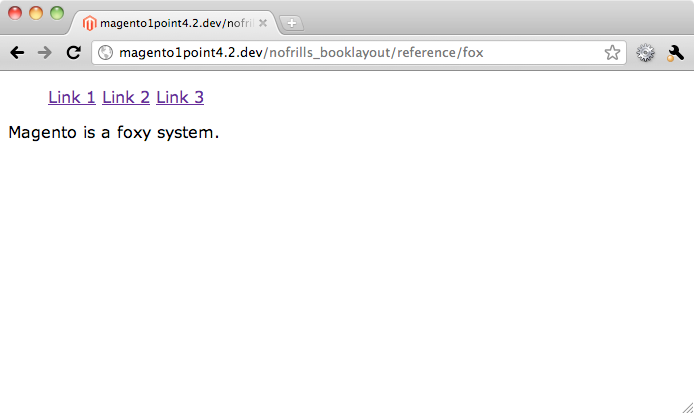
\includegraphics[width=1\textwidth]{images/chapter2/before.png}
\end{center}
\caption{}
%\label{fig:awesome_image}
\end{figure}


\subsection{After (\emph{Figure 2.4})}

\begin{figure}[htb]
\begin{center}
\leavevmode
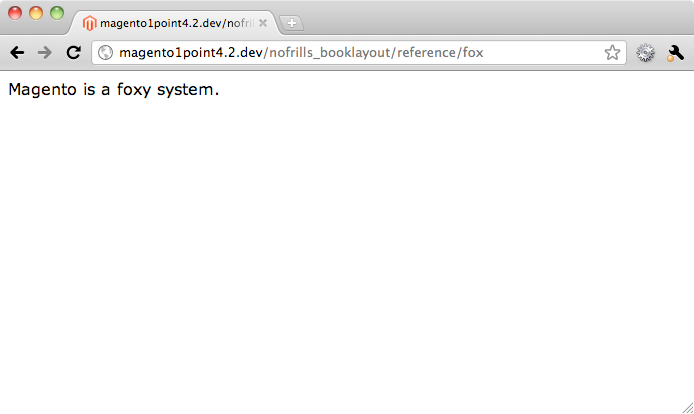
\includegraphics[width=1\textwidth]{images/chapter2/after.png}
\end{center}
\caption{}
%\label{fig:awesome_image}
\end{figure}


Remove instructions are processed in the \footnotesize\texttt{Mage\_Core\_Model\_Layout::generateXml} \normalsize  method.  This method

\begin{enumerate}
\item Combines all updates with a call to \footnotesize\texttt{\$xml = \$this-\textgreater getUpdate()-\textgreater asSimplexml();} \normalsize
\item Looks through the combined updates for any nodes named \footnotesize\texttt{remove}\normalsize.
\item If it finds a \footnotesize\texttt{remove} \normalsize  node, it then takes that node's name and looks for any \footnotesize\texttt{block} \normalsize  or \footnotesize\texttt{references} \normalsize  nodes with the same name.
\item If it finds any \footnotesize\texttt{blocks} \normalsize  or \footnotesize\texttt{references}\normalsize, these nodes are marked with an \footnotesize\texttt{ignore} \normalsize  attribute.
\item The \footnotesize\texttt{remove} \normalsize  blocks are ignored during the Layout rendering process.  Their job is to mark which nodes should be ignored.  After that, they're irrelevant
\end{enumerate}


Once the remove instructions have been processed, the resulting tree is set as the Page Layout.

This means in our most recent example we ended up with a Page Layout XML tree that looked exactly the same as before, with one exception

\begin{lstlisting}
<block type="nofrills_booklayout/template" name="sidebar" ignore="1">

\end{lstlisting}


When a \footnotesize\texttt{\textless block/\textgreater } \normalsize  or \footnotesize\texttt{\textless reference/\textgreater } \normalsize  has an \footnotesize\texttt{ignore="1"} \normalsize  attribute node, the Layout rendering process will \textbf{skip} that block.  In this way, the block, and all its sub-blocks, are removed from the final rendered page.

\section{What's Next}

So, we've now covered how to create and manage Page Layouts via XML files.  We've also explored Magento's "Update" mechanism, which allows us to build up Page Layout XML files via individuals Layout Update XML fragments, allowing for modular page layouts.

The final problems we need to solves are

\begin{enumerate}
\item How should we store \textbf{all} the layout update for our system
\item How should we automatically \textbf{load} these layout files into the system
\end{enumerate}


So far we've been using individual \footnotesize\texttt{\_init} \normalsize  methods in our controllers.  While this has offered us more modularity that previous methods, this will still get unwieldy as the number of controllers and actions grows.  Plus, there's still the sub-problem of how to create a method of doing this that allows back-end PHP developers and front-end PHP developers the ability to go about their jobs without crossing paths.

The answer to this question, and the final large topic we need to cover, is the Package Layout.

\emph{Visit http://www.pulsestorm.net/nofrills-layout-chapter-two to join the discussion online.}
\chapter{The Package Layout}
We're finally getting closer to fully understanding the Magento layout rendering process.  At the end of the last chapter, we stated that the final puzzle pieces were

\begin{enumerate}
\item How should we store \textbf{all} the layout update for our system
\item How should we \textbf{load} these layout files into the system
\end{enumerate}


The approach Magento has taken is to introduce \textbf{another} XML tree, this one called the \emph{Package Layout}.  The Package Layout is an XML tree which contains any number of Layout XML Update Fragments. The Package Layout contains \textbf{all the updates fragments} that the \textbf{entire application} might want to use.

The top level node in the package layout is named \footnotesize\texttt{\textless layouts/\textgreater }\normalsize.

\begin{lstlisting}
<layouts>
    <!-- ... --->
</layouts>

\end{lstlisting}


Make note of the plural, layout\textbf{s}.  This is different from the top level singular  \footnotesize\texttt{\textless layout/\textgreater } \normalsize  node of the Page Layout XML tree you were building in previous chapters.  That's because, as mentioned, this is a \textbf{different} XML tree.

The second level nodes of the Package Layout are not \footnotesize\texttt{blocks}\normalsize, or \footnotesize\texttt{references}\normalsize, or \textbf{any} tag we've seen so far.  The second level nodes are something new, called \emph{Handles}.  Each handle node contains a single XML Update Fragment.

\begin{lstlisting}
<layouts>
    <handle_name>
        <!-- ... XML Update Fragment --->
    </handle_name>

    <handle_name2>
        <!-- ... XML Update Fragment --->
    </handle_name2>

    <handle_name3>
        <!-- ... XML Update Fragment --->
    </handle_name3>

    <handle_name>
        <!-- ... XML Update Fragment --->
    </handle_name>

    <default> <!-- default is an actual handle name from the system-->
        <!-- ... -->
    </default>

    <catalog_product_send> <!-- another real name -->
        <!-- ... -->
    </catalog_product_send>


    <!-- etc. -->
</layouts>

\end{lstlisting}


Handle names may be repeated, but before we discuss what they mean, lets discuss how they're loaded into the system.

\section{The Why and Where of the Package Layout}

This collection of Layout Update XML nodes is called the Package Layout because it contains every possible Layout Update XML fragment that might be used in a particular design package.

Jumping back a few chapters, you'll remember that Magento stores its theme templates in the following location

\begin{lstlisting}
[BASE DESIGN FOLDER]/[AREA FOLDER]/[DESIGN PACKAGE FOLDER]/[THEME FOLDER]/template

\end{lstlisting}


Magento also stores its layout files in a similar location.

\begin{lstlisting}
[BASE DESIGN FOLDER]/[AREA FOLDER]/[DESIGN PACKAGE FOLDER]/[THEME FOLDER]/layout

\end{lstlisting}


Magento will look for layout files in this folder first.  If it doesn't find a specific layout file here, it will check the base fold at

\begin{lstlisting}
[BASE DESIGN FOLDER]/[AREA FOLDER]/base/default/layout

\end{lstlisting}


See Appendix E for more information on the \footnotesize\texttt{base} \normalsize  folder.

So, that's the \textbf{folder} where layout files are stored.  Where does Magento get the name of individual layout files?  Every individual code module in Magento has a \footnotesize\texttt{config.xml}\normalsize.  In this file, there's a node at

\begin{lstlisting}
<frontend>  <!-- frontend is the "area" name. -->
    <layout>
        <updates>
            <section>
                <file>section.xml</file>
            </section>
            <anysection>
                <file>anysection.xml</file>
            </anysection>
        </updates>
    </layout>
</frontend>

\end{lstlisting}


On each request, Magento will scan the config for any XML files located in the  \footnotesize\texttt{\textless updates\textgreater } \normalsize  node.  These filenames will be the files Magento will attempt to load up as the Package Layout.  The code that does this can be found in

\begin{lstlisting}
app/code/core/Mage/Core/Model/Layout/Update.php
Mage_Core_Model_Layout_Update::getFileLayoutUpdatesXml

\end{lstlisting}


The actual code in \footnotesize\texttt{getFileLayoutUpdatesXml} \normalsize  is pretty dense. However, you can approximate the code that grabs the list of files with something like this

\begin{lstlisting}
#URL: http://magento.example.com/nofrills_booklayout/reference/layoutfiles
public function layoutfilesAction()
{
    $updatesRoot = Mage::app()->getConfig()->getNode('frontend/layout/updates');
    $updateFiles = array();
    foreach ($updatesRoot->children() as $updateNode) {
        if ($updateNode->file) {
            $module = $updateNode->getAttribute('module');
            if ($module &&
            Mage::getStoreConfigFlag('advanced/modules_disable_output/' .
            $module)) {
                continue;
            }
            $updateFiles[] = (string)$updateNode->file;
        }
    }
    // custom local layout updates file - load always last
    $updateFiles[] = 'local.xml';
    var_dump($updateFiles);
}

\end{lstlisting}


Load the URL for the above action, and you'll see the list of files that Magento will load, and then combine, into the package layout.

Two additional things to note about the loading of the package layout.  First, you'll see in the above code, (which was copied from \footnotesize\texttt{Mage\_Core\_Model\_Layout\_Update::getFileLayoutUpdatesXml}\normalsize), that Magento checks for a config flag at \footnotesize\texttt{advanced/modules\_disable\_output} \normalsize  before loading any particular file.  This corresponds to the System Config section at

\begin{lstlisting}
System -> Configuration -> Advanced -> Disable Module's Output

\end{lstlisting}


If you've disabled a module's output through this config section, Magento will ignore loading that module's updates into the Package Layout.

The second thing you'll want to notice is this line

\begin{lstlisting}
// custom local layout updates file - load always last
$updateFiles[] = 'local.xml';

\end{lstlisting}


After loading XML files found in the configuration, Magento will add a \footnotesize\texttt{local.xml} \normalsize  file to the end of the list.  This file is where store owners can add their own Layout Update XML fragments to the Package Layout. We'll learn more about this later, but by loading \footnotesize\texttt{local.xml} \normalsize  last, Magento ensures any Layout Update XML Fragments here have the final say of what goes into the Layout.

Once Magento has determined which files should be loaded into the Package Layout, the contents of each file will be combined into a single, massive XML tree.

\section{Package Layout Examples}

As part of the module that came with this book, we've included a theme that \textbf{clears out} all most of the handles in the default Package Layout.  We've done this to provide some clarity in the examples below.  Unlike our examples so far, there's no public API for programmatically manipulating the Package Layout once its loaded.

You'll want to switch to this theme now.  We've placed this theme in the default package.  \textbf{IMPORTANT}: Doing this will make every part of your frontend cart produce a blank page.  It goes without saying, but bears repeating, don't do this with a production store.

If you go to

\begin{lstlisting}
System -> Configuration -> Design -> Package -> Current Package Name

\end{lstlisting}


and enter \footnotesize\texttt{default} \normalsize  (if it's not already there).  Next, go to

\begin{lstlisting}
System -> Configuration -> Design -> Themes -> Layout

\end{lstlisting}


and enter \footnotesize\texttt{nofrills\_layoutbook}\normalsize. Click \textbf{Save}, and you'll be set for the example in the next section, (see \emph{Figure 3.1})

\begin{figure}[htb]
\begin{center}
\leavevmode
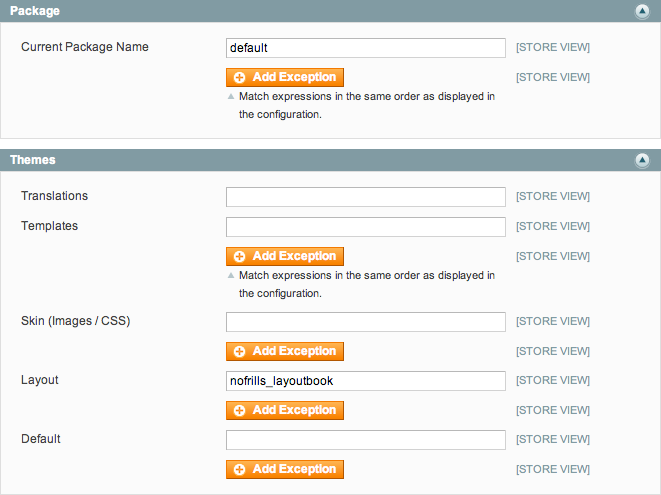
\includegraphics[width=1\textwidth]{images/chapter3/config-package.png}
\end{center}
\caption{}
%\label{fig:awesome_image}
\end{figure}


You can find your new "zeroed out" layout files at

\begin{lstlisting}
app/design/frontend/default/nofrills_layoutbook/layout/

\end{lstlisting}


If you load any page in your store, you'll encounter an empty, blank, and errorless browser screen.

\section{What is a Handle?}

Handles are used to organize the Layout Update XML fragments that your application needs.  Every time an HTTP request is sent to the Magento system, it generates handle names for the request.  There are some handle names which are produced on every request.  They include the handle \footnotesize\texttt{default}\normalsize, as well as a handle based on the controller's "Full Action Name" that was discussed in the previous chapter.

The Full Action Name, as a reminder, is a combination of the current module name, controller name, and action name.

\begin{itemize}
\item Module Name: \footnotesize\texttt{nofrills\_booklayout} \normalsize
\item Controller Name: \footnotesize\texttt{reference} \normalsize
\item Action Name: \footnotesize\texttt{fox} \normalsize
\end{itemize}


In the Package Layout example above, the

\begin{lstlisting}
<catalog_product_send>...</catalog_product_send>

\end{lstlisting}


node is an example of a full action name handle for the \textbf{send} Action in the \textbf{Product} controller of the \textbf{Catalog} module.

In general, it's the responsibility of the controller object to set handles for any particular request.  Also, you generally don't need to worry about setting your own handles.  Magento's base controller methods do this for you.  If you want to \textbf{see} the handles set from a particular action controller, use the following code snippet

\begin{lstlisting}
#URL: http://magento.example.com/nofrills_booklayout/reference/handle
public function handleAction()
{
    $this->loadLayout();
    $handles = Mage::getSingleton('core/layout')->getUpdate()->getHandles();
    var_dump($handles);
    exit;
}

\end{lstlisting}


You're probably wondering about the call to \footnotesize\texttt{\$this-\textgreater loadLayout();}\normalsize. Don't worry about it too much for now, we'll get to it soon enough.  Just know that that you need to call this method before being able to get a list of handles for a particular request.

\section{Rendering a Magento Layout}

So, we've finally arrived at the point where we have the vocabulary to fully explore how a Magento layout is created and then rendered for each request.  The rest of this chapter will explain that process in full.  From a high level, here's what happens

\begin{enumerate}
\item If it's not already cached, Magento loads the entire package layout into memory (from the individual XML file already discussed)
\item In the controller, the \footnotesize\texttt{loadLayout} \normalsize  method is called
\item In \footnotesize\texttt{loadLayout}\normalsize, Magento generates a list of "handles" for the request
\item In \footnotesize\texttt{loadLayout}\normalsize, Magento takes this list of handles, and uses them to search the Package Layout for a list of Layout XML Update Fragments
\item In \footnotesize\texttt{loadLayout}\normalsize, after fetching a list of Layout XML Update fragments, Magento checks those fragments for \footnotesize\texttt{\textless update name=""/\textgreater } \normalsize  tags.  If it finds any, it checks the package layout for any additional handles which match this tag
\item In \footnotesize\texttt{loadLayout}\normalsize, the Layout Update XML Fragments found in steps four and five are combined.  This combined XML tree is now the Page Layout
\item Magento uses the Page Layout to instantiate the needed block objects
\item In the controller, the \footnotesize\texttt{renderLayout} \normalsize  method is called.  This kicks off rendering of the Layout via its \footnotesize\texttt{getOutput} \normalsize  method.  The resulting output is added to a Magento Response object.
\end{enumerate}


Let's take a look at some concrete code examples. We'll be working in the following controller file.

\begin{lstlisting}
#File: app/code/local/Nofrills/Booklayout/controllers/PackageController.php
class Nofrills_Booklayout_PackageController extends
Mage_Core_Controller_Front_Action
{
    public function loadLayout($handles=null, $generateBlocks=true,
    $generateXml=true)
    {
        $original_results = parent::loadLayout($handles,$generateBlocks,
        $generateXml);

        $handles = Mage::getSingleton('core/layout')->getUpdate()->getHandles();
        echo "<strong>Handles Generated For This Request: ",
        implode(",",$handles),"</strong>";

        return $original_results;
    }

    #http://magento.example.com/nofrills_booklayout/package/index
    public function indexAction()
    {
        $this->loadLayout();
        $this->renderLayout();
    }
}

\end{lstlisting}


You'll notice we've extended the \footnotesize\texttt{loadLayout} \normalsize  method to print out the handles generated by Magento.  This is for our own debugging purposes.  Load up the index URL, and you should see a blank white page with only the handles listed, (see \emph{Figure 3.2})

\begin{figure}[htb]
\begin{center}
\leavevmode
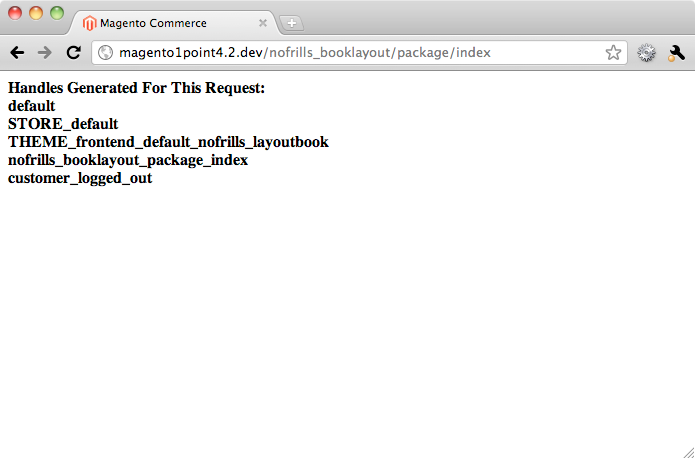
\includegraphics[width=1\textwidth]{images/chapter3/blank-with-handles.png}
\end{center}
\caption{}
%\label{fig:awesome_image}
\end{figure}


\section{Getting a Handle on Handles}

There's two handles you can always rely on being generated.  Those are the handle named \footnotesize\texttt{default}\normalsize, and the handle that's named for the "Full Action Name".

\begin{lstlisting}
default
nofrills_booklayout_package_index

\end{lstlisting}


Because of this, in the layout files that ship with Magento the handles for a page's structure are kept under the \footnotesize\texttt{\textless default/\textgreater } \normalsize  handle.  This is also where the "root" tag with the \footnotesize\texttt{output="toHtml"} \normalsize  attribute is stored. If you look at a stock \footnotesize\texttt{page.xml}\normalsize, you can see this.

\begin{lstlisting}
<!-- #File: app/design/frontend/base/default/layout/page.xml -->
<default translate="label" module="page">
    <label>All Pages</label>
    <block type="page/html" name="root" output="toHtml"
    template="page/3columns.phtml">

        <block type="page/html_head" name="head" as="head">
            <action method="addJs">
                <script>prototype/prototype.js</script>
            </action>
            <action method="addJs" ifconfig="dev/js/deprecation">
                <script>prototype/deprecation.js</script>
            </action>
            <action method="addJs">
                <script>lib/ccard.js</script>
            </action>
            ...

\end{lstlisting}


Layout Update XML Fragments located in the \footnotesize\texttt{default} \normalsize  handle will always be loaded.

If you look at our custom \footnotesize\texttt{page.xml}\normalsize, you'll see we've removed all the handle tags

\begin{lstlisting}
<!-- #File: app/design/frontend/default/nofrills_layoutbook/layout/page.xml -->
<?xml version="1.0"?>
<layout version="0.1.0">
</layout>

\end{lstlisting}


That's why our page is rendering blank. Let's restore those tags and see what effect it has.  We'll copy the base \footnotesize\texttt{page.xml} \normalsize  over our blank one.

\begin{lstlisting}
cp app/design/frontend/base/default/layout/page.xml \
app/design/frontend/default/nofrills_layoutbook/layout/page.xml

\end{lstlisting}


Clear your Magento cache and reload your page.  You should now see a base Magento layout, (see \emph{Figure 3.3})

\begin{figure}[htb]
\begin{center}
\leavevmode
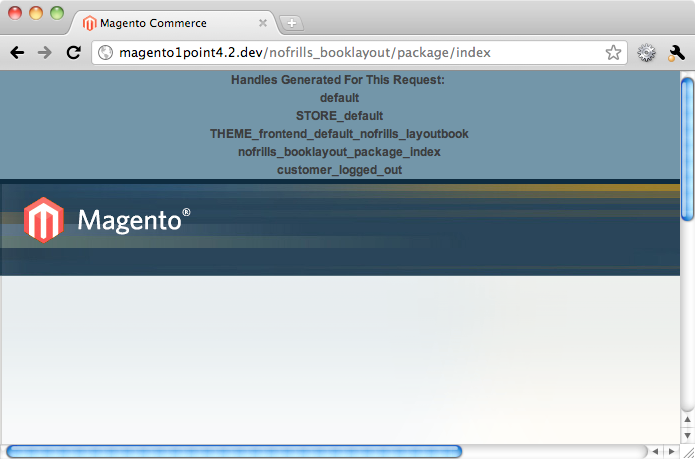
\includegraphics[width=1\textwidth]{images/chapter3/blank-theme.png}
\end{center}
\caption{}
%\label{fig:awesome_image}
\end{figure}


You'll want to either turn caching off or clear it between each page reload from here on out, see Appendix F for more information if you're interested in why.

Take a look at the top of page.xml and find the node named root

\begin{lstlisting}
#File: app/design/frontend/default/nofrills_layoutbook/layout/page.xml
<block type="page/html" name="root" output="toHtml"
template="page/3columns.phtml">

\end{lstlisting}


Let's edit this to remove the output tag

\begin{lstlisting}
<block type="page/html" name="root"
template="page/3columns.phtml">

\end{lstlisting}


Refresh your page (again, after clearing your cache).  The page now renders as blank.  You'd probably never do this for a production site, we've done here to demonstrate that the Magento Layout itself is built on the same concepts our simple templates from previous chapters.

Let's restore that output attribute before continuing

\begin{lstlisting}
<block type="page/html" name="root" output="toHtml"
template="page/3columns.phtml">

\end{lstlisting}


So, that's the \footnotesize\texttt{default} \normalsize  handle.  Any Layout Update XML fragments inside a default handle will always be a part of the Page Layout, and that's where most of the structural blocks live.  That brings us to the other handle you can always rely on being present, the Full Action Name handle.  In our examples above this is

\begin{lstlisting}
nofrills_booklayout_package_index

\end{lstlisting}


As previously mentioned, this handle is generated from the module name (\footnotesize\texttt{nofrills\_booklayout}\normalsize), the controller name (\footnotesize\texttt{package}\normalsize) and the action name (\footnotesize\texttt{index}\normalsize).  The handle will uniquely identify any request into the system.  Therefore, Layout Update XML fragments located in this handle are most often used to add content to the page.

Let's add a Layout Update XML fragment using our handle.  Open up the \footnotesize\texttt{local.xml} \normalsize  file, and paste in the following code.

\begin{lstlisting}
<!-- #File: app/design/frontend/default/nofrills_layoutbook/layout/local.xml -->
<?xml version="1.0"?>
<layout version="0.1.0">
    <nofrills_booklayout_package_index>
        <reference name="content">
            <block type="core/text" name="our_message">
                <action method="setText"><text>Hello Mars</text></action>
            </block>
        </reference>
    </nofrills_booklayout_package_index>
</layout>

\end{lstlisting}


Inside our \footnotesize\texttt{nofrills\_booklayout\_package\_index} \normalsize  node we've added a Layout Update XML fragment to update the content block with a little bit of text.  Reload, clear cache, and you can see our simple \emph{Hello Mars} text block has been added to the page.  However, if we move to this URL/Action

\begin{lstlisting}
#http://magento.example.com/nofrills_booklayout/package/second
public function secondAction()
{
    $this->loadLayout();
    $this->renderLayout();
}

\end{lstlisting}


We can see that our text block is, as expected, NOT added.  We'd need to add another handle to the Package Layout with its own Layout Update XML fragment for that to happen. Let's do that now.

\begin{lstlisting}
<!-- #File: app/design/frontend/default/nofrills_layoutbook/layout/local.xml -->
<layout version="0.1.0">
    <!-- ... -->
    <nofrills_booklayout_package_second>
        <reference name="content">
            <block type="core/text" name="our_message">
                <action method="setText"><text>Hello Jupiter</text></action>
            </block>
        </reference>
    </nofrills_booklayout_package_second>
    <!-- ... -->
</layout>

\end{lstlisting}


Notice the new handle's name (\footnotesize\texttt{nofrills\_booklayout\_package\_\textbf{second}}\normalsize) matches the \footnotesize\texttt{secondAction} \normalsize  method .  Refresh the page (after clearing your cache) and you'll see the Hello Jupiter text.

We can also use the Full Action Handle to change which template an existing block uses.  For example, to make this a one column layout, we'll get a reference to the root block and call its \footnotesize\texttt{setTemplate} \normalsize  method.

\begin{lstlisting}
<nofrills_booklayout_package_second>
    <reference name="content">
        <block type="core/text" name="our_message">
            <action method="setText"><text>Hello Jupiter</text></action>
        </block>
    </reference>

    <reference name="root">
        <action method="setTemplate">
            <template>page/1column.phtml</template>
        </action>
    </reference>
</nofrills_booklayout_package_second>

\end{lstlisting}


When editing a single Layout XML file, you can either put all your additional tags changes into a single handle, or spread them out. The following would be functionally the same as the above.

\begin{lstlisting}
<nofrills_booklayout_package_second>
    <reference name="content">
        <block type="core/text" name="our_message">
            <action method="setText"><text>Hello Jupiter</text></action>
        </block>
    </reference>
</nofrills_booklayout_package_second>

<nofrills_booklayout_package_second>
    <reference name="root">
        <action method="setTemplate">
            <template>page/1column.phtml</template>
        </action>
    </reference>
</nofrills_booklayout_package_second>

\end{lstlisting}


The order the update handles are placed in \textbf{is} significant. Consider multiple layout files that try to change a block's template.  The last file processed (\footnotesize\texttt{local.xml}\normalsize) will be the one that wins, just like the last method called on a PHP block wins

\begin{lstlisting}
$block->setTemplate('3columns.phtml');
$block->setTemplate('6columns.phtml');
$block->setTemplate('1column.phtml');

\end{lstlisting}


There's no firm rule in place here, but try not to have your layout action in one group of handles be too dependent on what's happened in another handle.

\section{More local.xml}

Just because we're in \footnotesize\texttt{local.xml} \normalsize  doesn't mean we're limited to Full Action Handles.  \textbf{Any} handle can be added to \textbf{any} Layout XML file, as all these files are combined into the Package Layout.  For example, we could add a default handle that would ensure the same content always gets added to the page in \footnotesize\texttt{local.xml} \normalsize

\begin{lstlisting}
<layout>
    <!-- ... -->
    <default>
        <reference name="content">
            <block type="core/text" name="for_everyone">
                <action method="setText">
                    <text>I am on all pages!</text>
                </action>
            </block>
        </reference>
    </default>

    <!-- ... -->
</layout>

\end{lstlisting}


\section{Adding Other Handles to the Page Layout}

There's one other tag you'll need to be aware of in the Package Layout.  You'll  often  want to use the same set of blocks over and over again for different Full Action Handles, similar to the way you'd use a simple subroutine or function in a full programming language.

To handle this situation there's an additional tag that the Package Layout understands named \footnotesize\texttt{\textless update/\textgreater }\normalsize.

When Magento is scanning the package layout for Layout Update XML fragments to use, it will do a secondary scan of those fragments for an \footnotesize\texttt{\textless update/\textgreater } \normalsize  tag.  If it finds one, it will \textbf{go back to the entire package layout} and grab any Layout Fragments that match the handle attribute.  Consider, based on our example above, the following \footnotesize\texttt{local.xml} \normalsize

\begin{lstlisting}
<layout version="0.1.0">
    <nofrills_booklayout_package_index>
        <reference name="content">
            <block type="core/text" name="planet_4">
                <action method="setText"><text>Hello Mars. </text></action>
            </block>
        </reference>

        <update handle="nofrills_booklayout_package_second" />
    </nofrills_booklayout_package_index>

    <nofrills_booklayout_package_second>
        <reference name="content">
            <block type="core/text" name="planet_5">
                <action method="setText"><text>Hello Jupiter. </text></action>
            </block>
        </reference>
    </nofrills_booklayout_package_second>

    <nofrills_booklayout_package_second>
        <reference name="root">
            <action method="setTemplate">
                <template>page/1column.phtml</template>
            </action>
        </reference>
    </nofrills_booklayout_package_second>
</layout>

\end{lstlisting}


If we loaded our index page here, the Page Layout would contain the following (sans comments)

\begin{lstlisting}
<!-- from our handle -->
<reference name="content">
    <block type="core/text" name="planet_4">
        <action method="setText"><text>Hello Mars. </text></action>
    </block>
</reference>

<!-- from our [update handle="nofrills_booklayout_package_second"/] -->
<reference name="root">
    <action method="setTemplate"><template>page/1column.phtml</template></action>
</reference>
<reference name="content">
    <block type="core/text" name="planet_5">
        <action method="setText"><text>Hello Jupiter. </text></action>
    </block>
</reference>

\end{lstlisting}


That's because while processing the \footnotesize\texttt{nofrills\_booklayout\_package\_index} \normalsize  handle, Magento encountered the \footnotesize\texttt{\textless update/\textgreater } \normalsize  tag.

\begin{lstlisting}
<update handle="nofrills_booklayout_package_second" />

\end{lstlisting}


By including this tag, we've told Magento that we \textbf{also} want to grab Layout Update XML fragments that are included in the \footnotesize\texttt{nofrills\_booklayout\_package\_second} \normalsize  handle.

You can think of this as a sort of "include" for Layout Update fragments. Magento itself uses this technique extensively.  For example, Magento defines the blocks for the \footnotesize\texttt{customer\_account\_login} \normalsize  handle, and then uses those again later on when it wants to include the same login on the multi-shipping checkout page.

\begin{lstlisting}
<checkout_multishipping_login>
    <update handle="customer_account_login"/>
</checkout_multishipping_login>

\end{lstlisting}


\section{Package Layout Term Review}

Phew!  That was a lot of new terminology to take in.  Let's close with a quick recap of the structure of our two XML trees, the Package Layout and the Page Layout

\subsection{Package Layout}

The Package Layout is an XML tree that contains all possible Layout XML Update Fragments for a design package.  Frangments are organized by handle.

\textbf{Top Level Node in the Package Layout}

\begin{itemize}
\item \footnotesize\texttt{\textless layouts\textgreater } \normalsize
\end{itemize}


\textbf{Allowed Second Level Nodes}

\begin{itemize}
\item Any arbitrary named node called a \footnotesize\texttt{handle} \normalsize
\end{itemize}


\textbf{Allowed Third Level Nodes}

\begin{itemize}
\item \footnotesize\texttt{\textless block\textgreater } \normalsize  or \footnotesize\texttt{\textless reference\textgreater }\normalsize, as the start of a Layout Update XML fragment
\item \footnotesize\texttt{\textless update\textgreater }\normalsize, used to include another handle's Layout XML Update Fragments
\end{itemize}


\subsection{Page Layout}

The Page Layout is the final collection of Layout Update XML Fragments used to create block objects for a request.

\textbf{Top Level Node in the Page Layout}

\begin{itemize}
\item \footnotesize\texttt{\textless layout\textgreater } \normalsize
\end{itemize}


\textbf{Allowed Second Level Nodes}

\begin{itemize}
\item \footnotesize\texttt{\textless block\textgreater } \normalsize
\item \footnotesize\texttt{\textless reference\textgreater } \normalsize
\item \footnotesize\texttt{\textless remove/\textgreater } \normalsize
\end{itemize}


\textbf{Allowed Third Level nodes}

\begin{itemize}
\item \footnotesize\texttt{\textless block\textgreater }\normalsize's and \footnotesize\texttt{\textless reference\textgreater }\normalsize's may contain - other blocks, or actions
\item \footnotesize\texttt{\textless remove/\textgreater } \normalsize
\end{itemize}


\textbf{Note}

\begin{itemize}
\item \footnotesize\texttt{\textless remove/\textgreater } \normalsize  is technically allowed anywhere, as the xpath expression used to parse it (\footnotesize\texttt{//remove}\normalsize) ends up searching the entire Page Layout.  Convention keeps it at the second nesting level
\end{itemize}


\subsection{Layout Update XML Fragment}

A partial XML document fragment that describes a series of PHP commands to run which may

\begin{itemize}
\item Create block objects
\item Insert block objects into other block objects
\item Reference block objects to call their methods
\end{itemize}


\emph{Visit http://www.pulsestorm.net/nofrills-layout-chapter-three to join the discussion online.}
\chapter{Bringing it All Together}
We've just spent the last three chapters reviewing some complicated concepts and \textbf{the interaction} of complicated concepts.  We're going to pause for a moment to review what we've learned, as well as provide an overall picture of how Magento builds a Page Layout.  Original drafts had this brief, mini-chapter at the start of the book, but it made people's head explode.  Hopefully it's safe enough to cover now

\section{How a Magento Layout is Built}

Somewhere in a controller action, the programmer creating the controller action method tells Magento that it's time to load the layout.  The end result of loading a layout is a Page Layout XML tree, (see \emph{Figure 4.1})

\begin{figure}[htb]
\begin{center}
\leavevmode
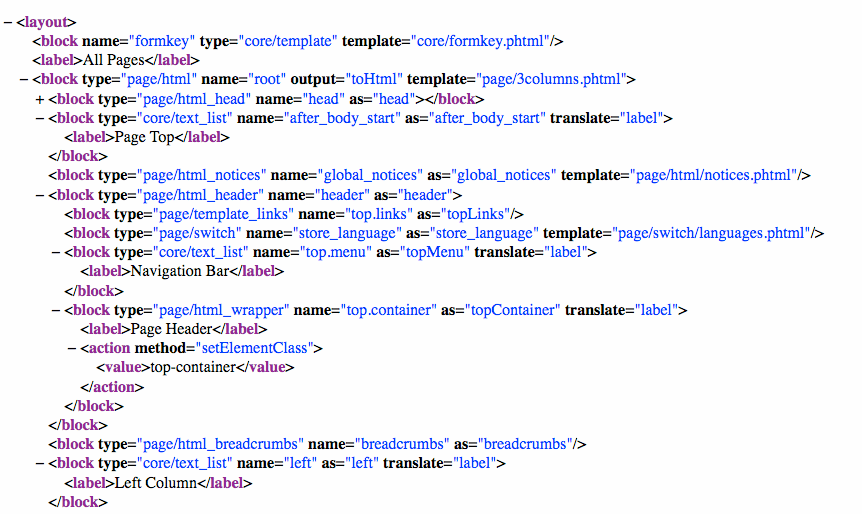
\includegraphics[width=1\textwidth]{images/chapter4/page-layout.png}
\end{center}
\caption{}
%\label{fig:awesome_image}
\end{figure}


To load a Page Layout, Magento will pick and choose Layout Update XML fragments from a repository of Layout Update XML fragments.  This repository of Layout Update XML fragments is known as the Package Layout. The Package Layout is loaded from disk by combining several XML files into a single tree, (see \emph{Figure 4.2})

\begin{figure}[htb]
\begin{center}
\leavevmode
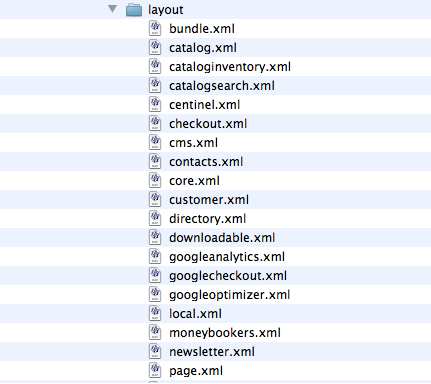
\includegraphics[width=1\textwidth]{images/chapter4/package-layout-files.png}
\end{center}
\caption{}
%\label{fig:awesome_image}
\end{figure}


Users of the Magento system can add to the Package Layout by

\begin{enumerate}
\item Creating and editing a \footnotesize\texttt{local.xml} \normalsize  file
\item Adding a custom XML file to the Layout via a module's \footnotesize\texttt{config.xml} \normalsize  file
\item Least desirably, but most commonly, editing or replacing existing Package Layout files in their their theme's layout
\end{enumerate}


The Package Layout organizes its many Layout Update XML fragments by handle.    During a normal page request life cycle, various parts of the Magento system will tell the Layout Update Manager that, when the time comes, Layout Update XML fragments from "handle x" should be loaded.  When the Controller Action developer tells Magento to load the layout, the Layout Update Manager checks this list, and asks the Package Layout for a copy of the Layout Update XML fragments contained within those particular handles.

Also, each fetched Layout Update XML fragment is processed at this time for an \footnotesize\texttt{\textless update handle="..."/\textgreater } \normalsize  node.  This node can be used to tell the manager to fetch \textbf{additional nodes} based on the specified handle.

Finally, a copy of all Layout Update XML fragments in hand, the Layout Update Manager combines them into a single XML tree.   This is the Page Layout.

\section{What is the Page Layout}

The Page Layout is a list of instruction for Magento.  Programmer types may call it a meta-programing language, or a domain-specific language.  Regardless of what you call, the last step of \textbf{loading} a Layout is for Magento to use the Page Layout to create and instantiate a nested tree of block objects.  These are PHP Objects, each one ultimately responsible for rendering a chunk of HTML.

That's the layout loaded.  The controller action programer may, at this point, choose to manipulate the layout object further.  This may include adding, removing, or setting properties on blocks.  The Magento Admin Console application does this regularly.  The Magento frontend (cart) application tends not to do this.  Irrespective of how, after loading a Layout and fiddling with it if they wish, the controller action developer then tells Magento it's time to render the layout object

\section{Rendering a Layout}

During the creation of Page Layout, certain Layout Update XML fragments marked certain blocks as "output blocks".  When we say certain blocks, this is almost always a single block, and equally almost always this is the block named \footnotesize\texttt{root}\normalsize.  This root block renders a page template.  This template, in turn, includes calls to render child blocks.  Some of these child blocks render via a template file, others are \footnotesize\texttt{core/text\_list} \normalsize  blocks which automatically render all their children.  Others render via pure PHP in the \footnotesize\texttt{\_toHtml} \normalsize  method.  This blocks rendering sub-blocks, rending sub-sub-blocks can continue many layers deep.

The end result of this  rendering is a single string variable containing all the HTML from the cascading render.  The string is then passed into a Magento response object, which is responsible for outputting the HTML page.

That, in a nutshell, is the Layout system.

\emph{Visit http://www.pulsestorm.net/nofrills-layout-chapter-four to join the discussion online.}
\chapter{Advanced Layout Features}
If you've absorbed the previous chapters of information, you have everything you need to be a skillful practitioner of Magento layouts.  Next we're going to cover some advanced features of the Layout system.  We'll be moving pretty fast so if you're getting frustrated stop, take a deep breath, and remember that this isn't hard, it's just different.  Once we're through, you'll be a true layout master.

\textbf{Note:} If you came here from Chapter 3, be sure to turn off the \footnotesize\texttt{nofrills\_layoutbook} \normalsize  theme.

\section{Action Parameters}

We've already covered calling Action Methods, but let's quickly review. During the loading of the layout and instantiation of the block object, the XML below

\begin{lstlisting}
<block type="some/foo" name="some_block">
    <action method="someMethod">
        <param1>a value</param1>
        <param2>27</param2>
    </action>
</block>

\end{lstlisting}


would run code something like the following

\begin{lstlisting}
$block = new Mage_Some_Block_Foo();
$block->someMethod('a value','27');

\end{lstlisting}


There are, however, a few extra features you can tap into while calling methods via blocks.  Let's take a look.

\section{Translation System}

Magento ships, out of the box, with a \footnotesize\texttt{gettext} \normalsize  like translation system.  This system allows you to define a number of symbols (usually the English language version of a phrase), and then conditionally swap in a translated phrase.  By default the action method parameters aren't run through this system, but it's possible (on an action by action basis) to tell Magento to translate certain parameters.

To indicate a parameter should be translated, you'd do something like

\begin{lstlisting}
<action method="someMethod" translate="param1" module="core">
    <param1>a value</param1>
    <param2>27</param2>
</action>

\end{lstlisting}


We've added two parameters to the \footnotesize\texttt{\textless action/\textgreater } \normalsize  node here. The first is

\begin{lstlisting}
translate="param1"

\end{lstlisting}


This tells Magento we want to run the \footnotesize\texttt{\textless param1/\textgreater } \normalsize  parameter through the translation engine.  In this case, that's the string "a value".  This is the reason each parameter is an extra node in the tree, it allows us to identify strings that need translation.  If you want to translate more than one parameter, the attribute will accept multiple names

\begin{lstlisting}
translate="param1 param2"

\end{lstlisting}


Next, we have

\begin{lstlisting}
module="core"

\end{lstlisting}


This tells Magento which module's data helper should be used to translate our strings.  Each module has (or should have) a helper class named Data.

\begin{lstlisting}
Mage_Core_Helper_Data
Mage_Catalog_Helper_Data

\end{lstlisting}


This helper can be instantiated via a call to the static helper method on the Mage object

\begin{lstlisting}
Mage::helper('core');       //shortcut for the one below
Mage::helper('core/data');

\end{lstlisting}


It's this helper object that has the translation function

\begin{lstlisting}
$h = Mage::helper('core');
$hello = $h->__('Hello');

//in the above scenario "$hello" might contain
//the string "Hola" if the spanish locale was loaded

\end{lstlisting}


The reason you need to specify a module for the translation helper is, each module can contain \textbf{its own} translations.  This allows different modules to translate their own symbols slightly differently based on context.

\section{Conditional Method Calling}

Another attribute you may see in the \footnotesize\texttt{\textless action/\textgreater } \normalsize  node is \footnotesize\texttt{ifconfig}\normalsize.

\begin{lstlisting}
<block type="page/html_head" name="head" as="head">
    <action method="addJs" ifconfig="dev/js/deprecation">
        <script>prototype/deprecation.js</script>
    </action>
</block>

\end{lstlisting}


This attribute can be used to tell Magento to \textbf{conditionally} call the specified method. The above XML is equivalent to PHP code something like

\begin{lstlisting}
$block = new Mage_Page_Block_Html_Head();
if(Mage::getStoreConfigFlag('dev/js/deprecation'))
{
    $block->addJs('prototype/deprecation.js');
}

\end{lstlisting}


That is, when you use the \footnotesize\texttt{ifconfig} \normalsize  attribute, you're telling Magento

\begin{quote}
Only make the following method call if the following System Configuration Variable returns true
\end{quote}

System Configuration variables can be set in the Admin Console under

\begin{lstlisting}
System -> Configuration

\end{lstlisting}


See Appendix I for more information of using the System Config system.

The \footnotesize\texttt{ifconfig} \normalsize  attribute is a powerful feature you can use to allow end users to selectively turn certain layout features on or off.  You can also use it to display different layout states based on the existing System Configuration values.

\section{Dynamic Parameters}

Magento also has the ability to pass \textbf{dynamic} parameters via Layout Update XML.  Normally, parameter values need to be fixed values

\begin{lstlisting}
<action method="someMethod" translate="param1" module="core">
    <param1>a value</param1>
    <param2>27</param2>
</action>

\end{lstlisting}


Above we're passing in the fixed values

\begin{lstlisting}
a value
27

\end{lstlisting}


However, consider the following alternate syntax.

\begin{lstlisting}
<action method="addLink" translate="label title" module="customer">
    <label>My Account</label>
    <url helper="customer/getAccountUrl"/>
    <title>My Account</title>
    <prepare/>
    <urlParams/>
    <position>10</position>
</action>

\end{lstlisting}


Here we're passing in three fixed values

\begin{lstlisting}
<label>My Account</label>
...
<title>My Account</title>
...
...
<position>10</position>

\end{lstlisting}


We're also passing in two null values

\begin{lstlisting}
...
...
...
<prepare/>
<urlParams/>
...

\end{lstlisting}


But there's one final parameter we're using with a syntax we haven't seen before

\begin{lstlisting}
...
<url helper="customer/getAccountUrl"/>
...
...
...
...

\end{lstlisting}


This \footnotesize\texttt{url} \normalsize  parameter tag is fetching data dynamically using Magento's helper classes.  When Magento encounters an action parameter with a helper attribute, it

\begin{enumerate}
\item Splits the helper by the last "/"
\item The first part of the split is used to instantiate the helper
\item The second part of the split is used as a method name
\item A helper is instantiated and the method from step \#3 is called.
\item The value returned by the method is used in the action method call
\end{enumerate}


So, that means the above XML translates into PHP code something like;

\begin{lstlisting}
$block;     //the block object
$h          = Mage:helper('customer'); //instantiate the customer data helper
$url        = $h->getAccountUrl();
$block->addLink('My Account',$url,'My Account',null,null,10);

\end{lstlisting}


Magento examines the \footnotesize\texttt{helper} \normalsize  attribute and splits off \footnotesize\texttt{getAccountUrl} \normalsize  to use as a method, leaving \footnotesize\texttt{customer} \normalsize  to be used to instantiate the helper class.  The helper is instantiated and \footnotesize\texttt{getAccountUrl} \normalsize  is called. The value returned from this method is then used as the parameter to pass to \footnotesize\texttt{addLink}\normalsize.

The above example uses the shorthand "data" helper format, but fear not. You can use \textbf{any} helper class alias to return a value. Consider the following example

\begin{lstlisting}
<action method="addLink" translate="label title" module="catalog"
ifconfig="catalog/seo/site_map">
    <label>Site Map</label>
    <url helper="catalog/map/getCategoryUrl" />
    <title>Site Map</title>
</action>

\end{lstlisting}


Here we're instantiating a \footnotesize\texttt{catalog/map} \normalsize  helper and calling its \footnotesize\texttt{getCategoryUrl} \normalsize  method.  The value which \footnotesize\texttt{getCategoryUrl} \normalsize  returns will be used in the call to the \footnotesize\texttt{addLink} \normalsize  method.

This powerful feature is the missing link for layout programming.  The ability to call into blocks with dynamic data parameters unlocks a world of potential for developers and designers alike.

\section{Ordering of Blocks}

Next up we have block ordering.  We'll be working in the following controller action

\begin{lstlisting}
#File: app/code/local/Nofrills/Booklayout/controllers/OrderController.php
class Nofrills_Booklayout_OrderController
extends Mage_Core_Controller_Front_Action
{
    public function indexAction()
    {
        $this->loadLayout();
        $this->renderLayout();
    }
}

\end{lstlisting}


Which corresponds to the URL

\begin{lstlisting}
http://magento.example.com/nofrills_booklayout/order

\end{lstlisting}


Consider the following \footnotesize\texttt{\textless nofrills\_booklayout\_order\_index\textgreater } \normalsize  update handle for our controller action.  You should know how to add this to your system by now, but if you don't putting it in your \footnotesize\texttt{local.xml} \normalsize  will do.  Review the previous chapters if you're unsure where \footnotesize\texttt{local.xml} \normalsize  is.

\begin{lstlisting}
<nofrills_booklayout_order_index>
    <reference name="content">
        <block type="core/text" name="one">
            <action method="setText">
                <text><![CDATA[<p>One</p>]]></text>
            </action>
        </block>
        <block type="core/text" name="two">
            <action method="setText">
                <text><![CDATA[<p>Two</p>]]></text>
            </action>
        </block>
        <block type="core/text" name="three">
            <action method="setText">
                <text><![CDATA[<p>Three</p>]]></text>
            </action>
        </block>
        <block type="core/text" name="four">
            <action method="setText">
                <text><![CDATA[<p>Four</p>]]></text>
            </action>
        </block>
        <block type="core/text" name="five">
            <action method="setText">
                <text><![CDATA[<p>Five</p>]]></text>
            </action>
        </block>
        <block type="core/text" name="six">
            <action method="setText">
                <text><![CDATA[<p>Six</p>]]></text>
            </action>
        </block>
        <block type="core/text" name="seven">
            <action method="setText">
                <text><![CDATA[<p>Seven</p>]]></text>
            </action>
        </block>
        <block type="core/text" name="line">
            <action method="setText">
                <text><![CDATA[<hr/>]]></text>
            </action>
        </block>
    </reference>
</nofrills_booklayout_order_index>

\end{lstlisting}


Loading up our page with this bit of Layout Update XML in place will give us a simple ordered list of paragraphs, followed by a line, (see \emph{Figure 5.1})

\begin{figure}[htb]
\begin{center}
\leavevmode
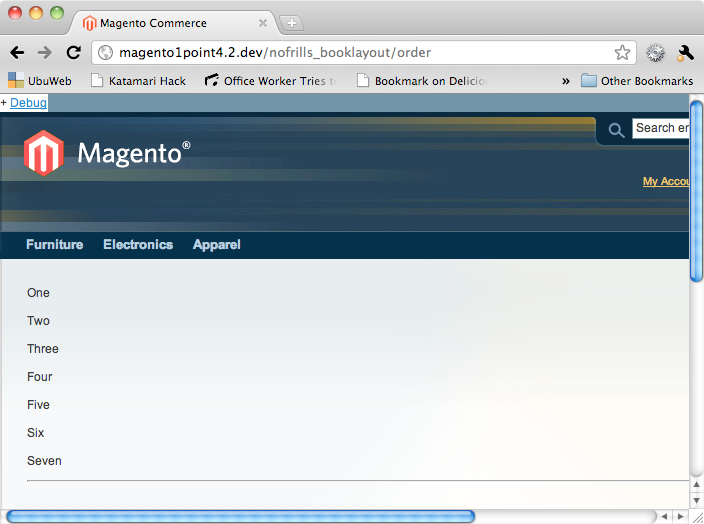
\includegraphics[width=1\textwidth]{images/chapter5/order-base.png}
\end{center}
\caption{}
%\label{fig:awesome_image}
\end{figure}


(We're using \footnotesize\texttt{\textless ![CDATA[\textless hr/\textgreater ]]\textgreater } \normalsize  nodes for our \footnotesize\texttt{setText} \normalsize  parameter. This allows us to insert HTML.)

Once you've got the above working, change your Layout Update XML such that an extra attribute named \footnotesize\texttt{before} \normalsize  is added to the block named line

\begin{lstlisting}
<block type="core/text" name="line" before="two">
    <action method="setText"><text><![CDATA[<hr/>]]></text></action>
</block>

\end{lstlisting}


Refresh your page.  The \footnotesize\texttt{\textless hr/\textgreater } \normalsize  element should now be rendered in between the "One" and "Two" paragraph, (see \emph{Figure 5.2})

\begin{figure}[htb]
\begin{center}
\leavevmode
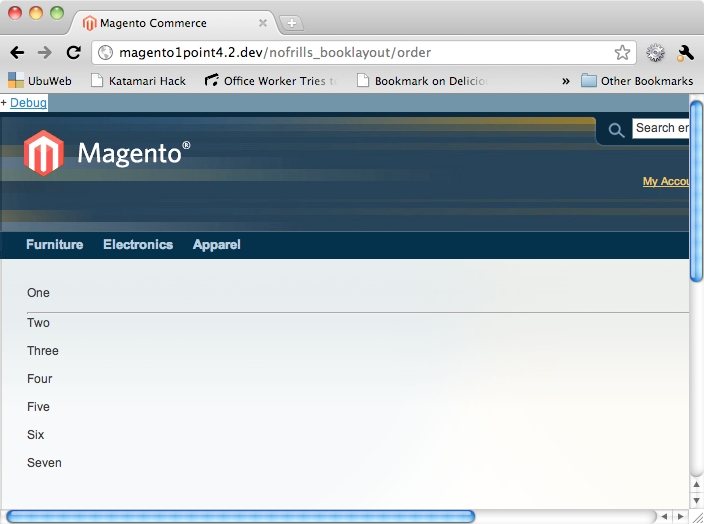
\includegraphics[width=1\textwidth]{images/chapter5/order-before-two.png}
\end{center}
\caption{}
%\label{fig:awesome_image}
\end{figure}


In plain english, the block \footnotesize\texttt{line} \normalsize  was inserted \footnotesize\texttt{before} \normalsize  the block \footnotesize\texttt{two}\normalsize.  There's also a corresponding after parameter.

\begin{lstlisting}
<block type="core/text" name="line" after="six">
    <action method="setText"><text><![CDATA[<hr/>]]></text></action>
</block>

\end{lstlisting}


Reload your page with the above in place, and your line block should render between six and seven.  If you want a block to be inserted last, just use

\begin{lstlisting}
<block type="core/text" name="line" after="-">

\end{lstlisting}


If, however, you want your block to be inserted first, use

\begin{lstlisting}
<block type="core/text" name="line" before="-">

\end{lstlisting}


The \footnotesize\texttt{before} \normalsize  and \footnotesize\texttt{after} \normalsize  attributes are most useful when you're inserting blocks into an existing set.  For example, with the above in place, we might have another Layout Update XML node somewhere that looked like

\begin{lstlisting}
<reference name="content">
    <block type="core/text" name="fakeline" after="four">
        <action method="setText">
            <text><![CDATA[<div style="border-color:black;
            border-style:solid;border-top:1px;width:300px;"></div>]]>
            </text>
        </action>
    </block>
</reference>

\end{lstlisting}


Assuming blocks one - seven had already been inserted, this bit of Layout Update XML would ensure your new block was inserted \footnotesize\texttt{after} \normalsize  the block named \footnotesize\texttt{four}\normalsize.  This feature makes working with a package or theme's default layout blocks far easier.

\section{Reordering Existing Blocks}

One thing that trips people up when dealing with block ordering is, you can only control where an individual block is inserted \textbf{at the time of insertion}.  Once you've inserted a block into the layout, it's "impossible" to change where it's rendered via the Layout XML files alone.

If you wanted to re-order a block that was already inserted, sometimes you can get away with removing it via the \footnotesize\texttt{unsetChild} \normalsize  method, and then reinserting it at the desired location

\begin{lstlisting}
<reference name="content">
    <action method="unsetChild"><name>one</name></action>
    <block type="core/text" name="one" after="-">
        <action method="setText"><t>one</t></action>
    </block>
</reference>

\end{lstlisting}


While this will sometimes work, if the block you're removing had children, or has data parameters set by other parts of the layout, you'll need to reset them after reinserting the block.  This makes the unset/re-insert method perilous at best, and should only be considered when all other options have been exhausted.

\section{Template Blocks Need Not Apply}

The \footnotesize\texttt{before} \normalsize  and \footnotesize\texttt{after} \normalsize  attributes work due to the way \footnotesize\texttt{core/text\_list} \normalsize  blocks automatically render their children

\begin{lstlisting}
class Mage_Core_Block_Text_List extends Mage_Core_Block_Text
{
    protected function _toHtml()
    {
        $this->setText('');
        foreach ($this->getSortedChildren() as $name) {
            $block = $this->getLayout()->getBlock($name);
            if (!$block) {
                Mage::throwException(Mage::helper('core')
                ->__('Invalid block: %s', $name));
            }
            $this->addText($block->toHtml());
        }
        return parent::_toHtml();
    }
}

\end{lstlisting}


The important line here is

\begin{lstlisting}
foreach ($this->getSortedChildren() as $name) {

\end{lstlisting}


This code is \footnotesize\texttt{foreach}\normalsize ing over a list of \textbf{sorted} children.  If you climb the chain back up to the \footnotesize\texttt{Mage\_Core\_Block\_Abstract} \normalsize     class, you can see that Magento keeps track of both children blocks, as well as a a sorted array of children

\begin{lstlisting}
/**
 * Contains references to child block objects
 *
 * @var array
 */
protected $_children = array();

/**
 * Sorted children list
 *
 * @var array
 */
protected $_sortedChildren = array();

\end{lstlisting}


So, while a \footnotesize\texttt{core/template} \normalsize  has this list of sorted children, the \footnotesize\texttt{before} \normalsize  and \footnotesize\texttt{after} \normalsize  attributes have no influence on a template block, as the order there is determined by where \footnotesize\texttt{\$this-\textgreater getChildHtml(...)} \normalsize  is called in the \footnotesize\texttt{phtml} \normalsize  template.

While it's beyond the scope of this book, an enterprising extension developer could probably create a class rewrite that would add a method to \footnotesize\texttt{core/text\_list} \normalsize  blocks allowing for an explicit reorder of the \footnotesize\texttt{\$\_sortedChildren} \normalsize  array. I wouldn't be surprised to see the feature crop up in a future version of Magento.

\section{Block Name vs. Block Alias}

There's one last block attribute we need to talk about, and that's the \footnotesize\texttt{as} \normalsize  attribute.

\begin{lstlisting}
<block type="sales/order_info" as="info" name="sales.order.info"/>

\end{lstlisting}


A block's name attribute defines its unique name in the layout object.  If present, the \footnotesize\texttt{as} \normalsize  attribute will define the block's alias in the layout.  If an alias is defined, you still interact with a block programmatically via its name.  The only time you use an alias is when rendering the block in a template.  For example, the above block's parent renders it with the following

\begin{lstlisting}
<?php $this->getChildHtml('info'); ?>

\end{lstlisting}


This allows someone programming Layout XML Updates to insert a different block to be rendered \textbf{without} changing the template. If you take a look at the \footnotesize\texttt{insert} \normalsize  method

\begin{lstlisting}
#File: app/code/core/Mage/Core/Block/Abstract.php
public function insert($block, $siblingName='', $after=false, $alias='')
{
    //...
    if ($block->getIsAnonymous()) {
        $this->setChild('', $block);
        $name = $block->getNameInLayout();
    } elseif ('' != $alias) {
        $this->setChild($alias, $block);
        $name = $block->getNameInLayout();
    } else {
        $name = $block->getNameInLayout();
        $this->setChild($name, $block);
    }
    //...
}

\end{lstlisting}


you can see if an alias is used that's the value that will be used to set the child block (and therefore the "template name").  Otherwise, Magento defaults to using the the block's name in the layout.

Block aliases are a feature you may never personally use, but recent versions of Magento have made \textbf{heavy} use of them to overcome some earlier design decisions. You'll want to make sure you're aware of the difference between an alias and name, even if you never use an alias in your own updates.

\section{Skipping a Child}

We've already covered the \footnotesize\texttt{getChildHtml} \normalsize  method in a previous chapter.  However, it has a cousin method named \footnotesize\texttt{getChildChildHtml}\normalsize.  This method is also defined on the \footnotesize\texttt{Mage\_Core\_Block\_Abstract} \normalsize  class

\begin{lstlisting}
public function getChildChildHtml($name, $childName = '', $useCache = true,
$sorted = false)
{
    if (empty($name)) {
        return '';
    }
    $child = $this->getChild($name);
    if (!$child) {
        return '';
    }
    return $child->getChildHtml($childName, $useCache, $sorted);
}

\end{lstlisting}


You use this method from a \footnotesize\texttt{phtml} \normalsize  template, and it might look something like

\begin{lstlisting}
<?php echo $this->getChildChildHtml('my_child', 'foo'); ?>

\end{lstlisting}


The \footnotesize\texttt{getChildHtml} \normalsize  method will render out the specified child.  The \footnotesize\texttt{getChildChildHtml} \normalsize  method obtains a reference to the first child block (\footnotesize\texttt{my\_child} \normalsize  above), and then calls \footnotesize\texttt{getChildHtml} \normalsize  on it.

This method is most useful when you're editing a \footnotesize\texttt{phtml} \normalsize  template and don't want to restructure your blocks.  I personally haven't found much use for it, but you will see it used in the wild and in the core, so it's worth knowing about.  The most typical use is to render a \footnotesize\texttt{core/template} \normalsize  block as though it was a \footnotesize\texttt{core/text\_list} \normalsize  block.

\emph{Visit http://www.pulsestorm.net/nofrills-layout-chapter-five to join the discussion online.}
\chapter{CMS Pages}
This chapter covers the CMS Page feature.  For day-to-day Magento work most of the knowledge here is unnecessary.  However, if you ever need to debug a Magento CMS page render, or are curious how CMS pages interact with the layout, this is the chapter for you.  We'll also being laying the groundwork for our final chapter on Widgets.

Back in 1996, if you wanted to put a piece of content online, you just uploaded an HTML file.  If you were really savvy, you'd upload an HTML \textbf{include} file that contained your content, and the HTML page itself would use server side includes.

It's weird, that in 2011, if you asked a developer how to add some content to a site or a web application, their process would be almost exactly the same.  Instead of adding an HTML file, they'd add a controller and a template, and then put the HTML content in the template.

However, for \textbf{non-developers}, managing content on a website has gone completely GUI.  Systems like Drupal, Concrete5, and Joomla rule the roost.  Users expect to manage their sites via a user interface, and \emph{not} via code or adding files.  Magento's often overlooked CMS features allows users the control they want. Don't worry though, there's plenty in the CMS for a developer to sink their teeth into, particularly a developer who knows the layout system inside out.

\section{Creating a Page}

The CMS starts with a CMS Page entity. If you browse to

\begin{lstlisting}
CMS -> Pages

\end{lstlisting}


in the Admin Console, you'll see a list of CMS pages that have already been added to the system, (see \emph{Figure 5.1})

\begin{figure}[htb]
\begin{center}
\leavevmode
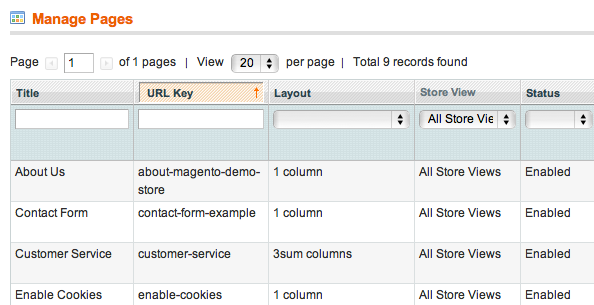
\includegraphics[width=1\textwidth]{images/chapter6/cms-page.png}
\end{center}
\caption{}
%\label{fig:awesome_image}
\end{figure}


If you click on "Add New Page" you'll be presented with a standard Magento editing UI, allowing you to enter information and create your page, (see \emph{Figure 5.2})

\begin{figure}[htb]
\begin{center}
\leavevmode
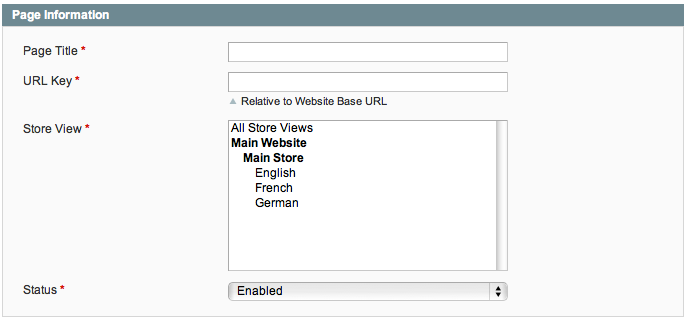
\includegraphics[width=1\textwidth]{images/chapter6/page-info.png}
\end{center}
\caption{}
%\label{fig:awesome_image}
\end{figure}


Let's create a simple page by entering the following values.  Don't worry about the specifics right now, we'll get to them down below

\begin{lstlisting}
[Page Information : Page Title]     Our Hello World Page
[Page Information : URL Key]        hello-world
[Page Information : Store View]     All Store Views
[Page Information : Status]         Enabled

[Content: Content Heading]          Welcome World!
[Content: Editor]                   The quick brown fox jumps over the lazy dog.

\end{lstlisting}


Once you're done, click on save and Next, load up the following URL in your browser

\begin{lstlisting}
http://magento.example.com/hello-world

\end{lstlisting}


You should see your new CMS page, (see \emph{Figure 5.3})

\begin{figure}[htb]
\begin{center}
\leavevmode
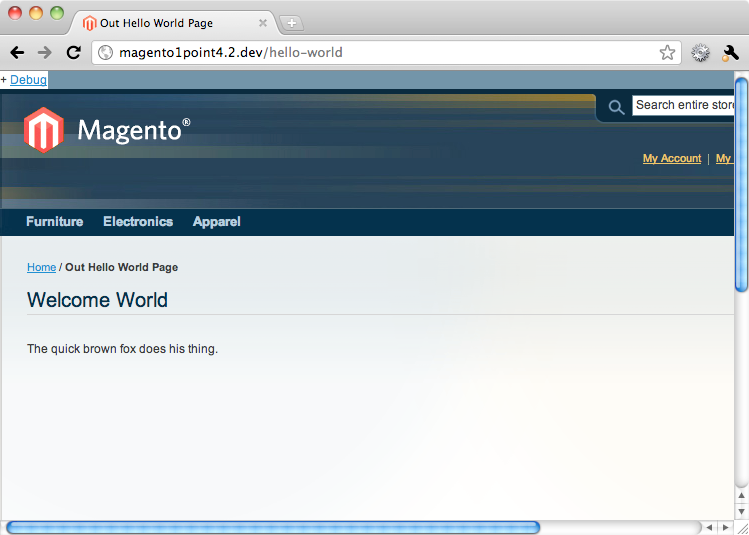
\includegraphics[width=1\textwidth]{images/chapter6/page1.png}
\end{center}
\caption{}
%\label{fig:awesome_image}
\end{figure}


When you saved your page in the admin, Magento stored all that data as a \footnotesize\texttt{cms/page} \normalsize  model.

\begin{lstlisting}
$page = Mage::getModel('cms/page');

\end{lstlisting}


When Magento identifies a URL as a CMS page, it loads this model up, reads its information, and then displays it to the page.

Let's take a look at all of the CMS Page fields and briefly describe what they do.

\subsection{Page Information : Page Title}

This is the title of your CMS page.  It will display in the Admin Console grid, your page's \footnotesize\texttt{\textless title/\textgreater } \normalsize  tag, and the default breadcrumb display.

\subsection{Page Information : URL Key}

This is the non-server portion of your page URL.  This can be any string that's valid in a URL.  In our example above, we used

\begin{lstlisting}
hello-world

\end{lstlisting}


If we had used

\begin{lstlisting}
hello-world.html

\end{lstlisting}


our page URL would have been

\begin{lstlisting}
http://magento.example.com/hello-world.html

\end{lstlisting}


\subsection{Page Information : Store View}

This setting determines which stores your page may appear in.  This allows you to hide content from stores where it may not be appropriate, or provide different version of a page for different stores.

Stores here is referring to Magento's internal abstract "Store" concept.

\subsection{Page Information : Status}

The status field allows you to disable or enable a page.  A disabled page will return a response with a 404 HTTP Status code.  This is great for embargoed content, or for saving seasonal content to use over again.

\subsection{Content: Content Heading}

The content heading determines your page's top level \footnotesize\texttt{\textless h1/\textgreater } \normalsize  tag. (See rendering section below for more information).

\subsection{Content: Editor}

This is the rich text editor where you enter your page's content.  In addition to the various formatting buttons common to most rich text editors, clicking the Show/Hide Editor button will toggle the raw source view.  When viewing a page in raw source view, you can view and edit the actual HTML that will render your page.

Also in raw source view, you'll see a few additional buttons. Insert Widget, Insert Image, and Insert Variable.  Clicking one these buttons eventually results in text something like

\begin{lstlisting}
{{config path="trans_email/ident_general/email"}}

\end{lstlisting}


being added to your raw source. This is a directive tag, and we'll cover it in greater detail in just a bit.

\subsection{Meta : Keywords}

The text in this field controls the \footnotesize\texttt{\textless meta name="keywords"/\textgreater } \normalsize  tag on your page.  The contents of this field will be added directly to the \footnotesize\texttt{content} \normalsize  attribute of the tag.

\begin{lstlisting}
<meta name="keywords" content="This is a test of the keywords." />

\end{lstlisting}


\subsection{Meta : Description}

Much like \textbf{Keywords}, the \textbf{Description} field controls the contents of your page's \footnotesize\texttt{\textless meta name="description"/\textgreater } \normalsize  tag.

\begin{lstlisting}
<meta name="description" content="Describing the meta." />

\end{lstlisting}


\subsection{Design : Layout}

This select box allows you to set which page structure template your CMS page will use. This select is populated by a call to

\begin{lstlisting}
//Mage_Page_Model_Source_Layout
Mage::getSingleton('page/source_layout')->toOptionArray()

\end{lstlisting}


which, in a default installation, ultimately reads from the global config nodes at the following location

\begin{lstlisting}
<config>
    <global>
        <cms>
            <page>
                ...
            </page>
        </cms>
    </global>
</config>

\end{lstlisting}


You can take a look at the structure in

\begin{lstlisting}
app/code/core/Mage/Page/etc/config.xml

\end{lstlisting}


for an idea on what Magento expects to find in there

\begin{lstlisting}
<page>
    <layouts>
        <empty module="page" translate="label">
            <label>Empty</label>
            <template>page/empty.phtml</template>
            <layout_handle>page_empty</layout_handle>
        </empty>
        <one_column module="page" translate="label">
            <label>1 column</label>
            <template>page/1column.phtml</template>
            <layout_handle>page_one_column</layout_handle>
            <is_default>1</is_default>
        </one_column>
        <two_columns_left module="page" translate="label">
            <label>2 columns with left bar</label>
            <template>page/2columns-left.phtml</template>
            <layout_handle>page_two_columns_left</layout_handle>
        </two_columns_left>
        <two_columns_right module="page" translate="label">
            <label>2 columns with right bar</label>
            <template>page/2columns-right.phtml</template>
            <layout_handle>page_two_columns_right</layout_handle>
        </two_columns_right>
        <three_columns module="page" translate="label">
            <label>3sum columns</label>
            <template>page/3columns.phtml</template>
            <layout_handle>page_three_columns</layout_handle>
        </three_columns>
    </layouts>
</page>

\end{lstlisting}


If you can hold on, you'll eventually understand to the meaning of all the tags above. For now, if you take a peek at the HTML source for that select

\begin{lstlisting}
<select id="page_root_template" name="root_template"
class="required-entry select">
    <option value="empty">Empty</option>
    <option value="one_column" selected="selected">1 column</option>
    <option value="two_columns_left">2 columns with left bar</option>
    <option value="two_columns_right">2 columns with right bar</option>
    <option value="three_columns">3sum columns</option>
</select>

\end{lstlisting}


you can see that Magento's taking the \textbf{tag names} from the above nodes for option values.  This is what Magento will save with its page model, and will then use later to retrieve the label, template, and layout\_handle values.

\subsection{Design : Layout Update XML}

The Magento CMS system still uses the layout/block mechanism for page rendering.  This field will allow you to add additional Layout Update XML fragments to your Page Layout for a CMS Page request.  For example, you could add an additional text content block if you liked with

\begin{lstlisting}
<reference name="content">
    <block type="core/text" name="redundant">
        <action method="setText"><text>Hello Again</text></action>
    </block>
</reference>

\end{lstlisting}


\subsection{Design : Custom Design}

Fields in this section allow users to override the above values, and our default theme, for specific date ranges.

\section{CMS Page Rendering}

Overview out of the way, let's get to those seemingly confusing abstractions!  You're probably wondering how Magento knows a particular request should be rendered with a CMS Page.  If you're a certain kind of developer, you're wondering how Magento routes a URL to the CMS rendering routines, (which is just a different way of saying the same thing)

When a URL request comes into Magento, the first thing Magento asks itself is

\begin{quote}
Based on my current configuration, should this URL be handled by an admin controller?
\end{quote}

If the answer is yes, Magento dispatches to the appropriate admin action controller. If not, the next thing Magento asks itself is

\begin{quote}
Based on my current configuration, should this URL be handled by a frontend controller action?
\end{quote}

If the answer is yes, Magento dispatches to the appropriate action controller.   If the answer is no, Magento asks itself one last question

\begin{quote}
Looking at that URL, is there a CMS page that matches its key/identifier?
\end{quote}

If so, manually set \textbf{the request's} module, controller, and action.  Also, add a parameter with the page ID.  The Page ID is the database ID of the \footnotesize\texttt{cms/page} \normalsize  object.  The code that does this looks something like

\begin{lstlisting}
    $request->setModuleName('cms')
        ->setControllerName('page')
        ->setActionName('view')
        ->setParam('page_id', $pageId);

\end{lstlisting}


By doing this, Magento will automatically dispatch to the following controller action.

\begin{lstlisting}
Mage_Cms_PageController::viewAction

\end{lstlisting}


If you're interested in checking out the code that looks for a CMS page, checkout the \footnotesize\texttt{match} \normalsize  method in

\begin{lstlisting}
#File: app/code/core/Mage/Cms/Controller/Router.php
public function match(Zend_Controller_Request_Http $request)
{
    ...
}

\end{lstlisting}


\section{Index Page}

The one exception to the routing scenario described above is the special root page of a site, alternately called the "index" page or the "home" page.

\begin{lstlisting}
http://magento.example.com/

\end{lstlisting}


Magento URLs that lack ANY path portion (that is, they contain only a server name) will be dispatch to the following controller action.

\begin{lstlisting}
Mage_Cms_IndexController::indexAction

\end{lstlisting}


This check happens \textbf{after} the check for a standard controller is instantiated, but \textbf{before} the CMS Page check is done.

You can override which controller the index page dispatches to via the System Config variable

\begin{lstlisting}
System -> Configuration -> Web -> Default Pages -> Default Web Url

\end{lstlisting}


In a base install, this value is \footnotesize\texttt{cms}\normalsize.  What that means is, when you go to the root level page, Magento will treat it as though you've gone to

\begin{lstlisting}
http://magento.example.com/cms

\end{lstlisting}


If you wanted to have a particular category page display as the home page, you could set this value to something like \footnotesize\texttt{catalog/category/view/id/8}\normalsize.

\section{What You \textbf{Need} to Know}

That was some heavy abstract lifting back there.  If you're not interested in those kind of details, all you really need to know can be summed up by the following

\begin{quote}
If Magento decides a URL needs a CMS page, it dispatches to \footnotesize\texttt{Mage\_Cms\_PageController::viewAction} \normalsize
\end{quote}

Let's take a look at that controller

\begin{lstlisting}
#File: app/code/core/Mage/Cms/controllers/PageController.php
class Mage_Cms_PageController extends Mage_Core_Controller_Front_Action
{
    /**
     * View CMS page action
     *
     */
    public function viewAction()
    {
        $pageId = $this->getRequest()
            ->getParam('page_id', $this->getRequest()->getParam('id', false));
        if (!Mage::helper('cms/page')->renderPage($this, $pageId)) {
            $this->_forward('noRoute');
        }
    }
}

\end{lstlisting}


That's only four lines in the method body, but if you're not familiar with Magento coding conventions, it's four dense looking lines.  We're going to tease apart what's going on in this method. If you're already familiar with Magento conventions you may want to skip ahead (although reviewing information never hurt anyone)

The call to \footnotesize\texttt{\$this-\textgreater getRequest()} \normalsize  returns the Magento request object.  Rather than have you interact directly with \footnotesize\texttt{\$\_GET}\normalsize, \footnotesize\texttt{\$\_POST} \normalsize  and \footnotesize\texttt{\$\_COOKIES}\normalsize, Magento provides a request object that allows you access to the same information.  This object is a \footnotesize\texttt{Mage\_Core\_Controller\_Request\_Http}\normalsize, which extends from a Zend class (\footnotesize\texttt{Zend\_Controller\_Request\_Http}\normalsize)

Next, we're chaining in a call to \footnotesize\texttt{getParam} \normalsize  in order to retrieve the value of \footnotesize\texttt{page\_id}\normalsize.  This is the id of our \footnotesize\texttt{cms/page} \normalsize  model.  The second parameter to \footnotesize\texttt{getParam} \normalsize  is a default value to return if \footnotesize\texttt{page\_id} \normalsize  isn't found.  In this case, we're calling \footnotesize\texttt{getParam} \normalsize  \textbf{again}, this time looking for value of the id parameter.  If there's no id parameter, \footnotesize\texttt{\$pageId} \normalsize  is set to false.

So, we now have our page id.  Next,

\begin{lstlisting}
if (!Mage::helper('cms/page')->renderPage($this, $pageId)) {
    $this->_forward('noRoute');
}

\end{lstlisting}


we instantiate a \footnotesize\texttt{cms/page} \normalsize  helper class, and call its render method.  We pass in a reference to the controller, and the page id we just fetched from the request.

If this method returns false, we forward on to \footnotesize\texttt{noRoute}\normalsize, which for our purposes we'll call the 404 Page.

\section{Where's the Layout?}

Earlier we mentioned the CMS system used the same layout rendering engine as the rest of Magento.  However, you're probably wondering where the calls to \footnotesize\texttt{\$this-\textgreater loadLayout()} \normalsize  and \footnotesize\texttt{\$this-\textgreater renderLayout()} \normalsize  are.  You may also be wondering why we're doing something weird like passing a reference to the Controller (\footnotesize\texttt{\$this}\normalsize) to our \footnotesize\texttt{cms/page} \normalsize  helper.

The answers to both questions lies within the \footnotesize\texttt{renderPage} \normalsize  method, so lets take a look

\begin{lstlisting}
#File: app/code/core/Mage/Cms/Helper/Page.php
class Mage_Cms_Helper_Page extends Mage_Core_Helper_Abstract
{
    public function renderPage(Mage_Core_Controller_Front_Action $action,
    $pageId = null)
    {
        return $this->_renderPage($action, $pageId);
    }

    ...

    protected function _renderPage(
        Mage_Core_Controller_Varien_Action  $action, $pageId = null,
        $renderLayout = true)
    {
        ...

        $action->loadLayoutUpdates();
        $layoutUpdate = ($page->getCustomLayoutUpdateXml() && $inRange)
        ? $page->getCustomLayoutUpdateXml() : $page->getLayoutUpdateXml();
        $action->getLayout()->getUpdate()->addUpdate($layoutUpdate);
        $action->generateLayoutXml()->generateLayoutBlocks();

        ...

        if ($renderLayout) {
            $action->renderLayout();
        }

    }
}

\end{lstlisting}


We've truncated much of the actual code (...) to focus on the specific lines above.  You'll see that the \footnotesize\texttt{renderPage} \normalsize  method wraps a call to the internal, protected \footnotesize\texttt{\_renderPage} \normalsize  method.  Notice that the controller we've passed in is (locally) known as \footnotesize\texttt{\$action}\normalsize.  Without going into too much detail, the code above replaces your calls to \footnotesize\texttt{\$this-\textgreater loadLayout()}\normalsize.

In fact, if you looked at the implementation of the \footnotesize\texttt{loadLayout} \normalsize  method in the base action controller, you'd see code similar to what's above.  The only difference here is, after loading the layout update handles from the package layout files, we then add any additional layout handles from our CMS Page. (You'll recall that Admin Console allowed us to add layout update handles for specific CMS pages)

We won't go into every little detail of the page rendering process, but we will highlight a few other chunks of code that should shed some light on what we were doing in the Admin Console GUI.

\section{Adding the CMS Blocks}

Take a look at the following line

\begin{lstlisting}
    $action->getLayout()->getUpdate()
        ->addHandle('default')
        ->addHandle('cms_page');

\end{lstlisting}


Here, the handle \footnotesize\texttt{cms\_page} \normalsize  is being issued.  This means when we're pulling Layout Update XML from the package layout, the following will be included.

\begin{lstlisting}
<!-- File: app/design/frontend/base/default/layout/cms.xml -->
<layout>
    <!-- ... -->
    <cms_page translate="label">
        <label>CMS Pages (All)</label>
        <reference name="content">
            <block type="core/template" name="page_content_heading"
            template="cms/content_heading.phtml"/>
            <block type="page/html_wrapper" name="cms.wrapper" translate="label">
                <label>CMS Content Wrapper</label>
                <action method="setElementClass"><value>std</value></action>
                <block type="cms/page" name="cms_page"/>
            </block>
        </reference>
    </cms_page>
    <!-- ... --->
</layout>

\end{lstlisting}


This is the key Layout Update XML for CMS pages.  It adds the blocks for the content heading, and the page content itself, to the page layout.  Later on in the render method we set the page content header by grabbing the saved content header values from our page model

\begin{lstlisting}
$contentHeadingBlock = $action->getLayout()->getBlock('page_content_heading');
if ($contentHeadingBlock) {
    $contentHeadingBlock->setContentHeading($page->getContentHeading());
}

\end{lstlisting}


This value is then referenced in the content heading block's template \footnotesize\texttt{cms/content\_heading.phtml}\normalsize.

\section{Setting the Page Template}

You may remember configuring a page template in the GUI. This template is stored in the root\_template property, and Magento uses it here

\begin{lstlisting}
if ($page->getRootTemplate()) {
    $action->getLayout()->helper('page/layout')
        ->applyTemplate($page->getRootTemplate());
}

\end{lstlisting}


The Layout object's \footnotesize\texttt{applyTemplate} \normalsize  method takes the saved value (say, \footnotesize\texttt{two\_columns\_left}\normalsize), jumps back into the config to find the name of the template it should set, and then sets it.

\begin{lstlisting}
public function applyTemplate($pageLayout = null)
{
    if ($pageLayout === null) {
        $pageLayout = $this->getCurrentPageLayout();
    } else {
        $pageLayout = $this->_getConfig()->getPageLayout($pageLayout);
    }

    if (!$pageLayout) {
        return $this;
    }

    if ($this->getLayout()->getBlock('root') &&
        !$this->getLayout()->getBlock('root')->getIsHandle()) {
            // If not applied handle
            $this->getLayout()
                ->getBlock('root')
                ->setTemplate($pageLayout->getTemplate());
    }

    return $this;
}

\end{lstlisting}


You'll remember that the \footnotesize\texttt{two\_columns\_left} \normalsize  config node looked something like this

\begin{lstlisting}
<two_columns_left module="page" translate="label">
    <label>2 columns with left bar</label>
    <template>page/2columns-left.phtml</template>
    <layout_handle>page_two_columns_left</layout_handle>
</two_columns_left>

\end{lstlisting}


You can see we're using the \footnotesize\texttt{\textless template/\textgreater } \normalsize  node above, but we don't seem to be using the \footnotesize\texttt{\textless layout\_handle/\textgreater } \normalsize  anywhere.  Plus, there's the \footnotesize\texttt{getIsHandle} \normalsize  method call above.  What's that all about?

Other parts of the system will add a layout handle named after the values in the \footnotesize\texttt{\textless layout\_handle\textgreater } \normalsize  tag. If you look at one of these handles

\begin{lstlisting}
<page_two_columns_left translate="label">
    <label>All Two-Column Layout Pages (Left Column)</label>
    <reference name="root">
        <action method="setTemplate">
            <template>page/2columns-left.phtml</template>
        </action>
        <!-- Mark root page block that template is applied -->
        <action method="setIsHandle"><applied>1</applied></action>
    </reference>
</page_two_columns_left>

\end{lstlisting}


you can see it's applying a template via the \footnotesize\texttt{setTemplate} \normalsize  method, and also setting a \footnotesize\texttt{IsHandle} \normalsize  flag on the object.  This flag is used internally by the block to prevent multiple handles from setting the root template.  This isn't done by the CMS Page render, but it's good to know about.

\section{Rendering the Content Area}

So that covers some of the ancillary items around rendering a CMS page, but what about the page content itself?  We've added a \footnotesize\texttt{cms/page} \normalsize  block named \footnotesize\texttt{cms\_page} \normalsize  using the \footnotesize\texttt{cms\_page} \normalsize  handle, but we don't seem to do anything with it.

That's because the CMS block itself does the rendering.  If you take a look at its \footnotesize\texttt{\_toHtml} \normalsize  method

\begin{lstlisting}
class Mage_Cms_Block_Page extends Mage_Core_Block_Abstract
{
    //...
    protected function _toHtml()
    {
        /* @var $helper Mage_Cms_Helper_Data */
        $helper = Mage::helper('cms');
        $processor = $helper->getPageTemplateProcessor();
        $html = $processor->filter($this->getPage()->getContent());
        $html = $this->getMessagesBlock()->getGroupedHtml() . $html;
        return $html;
    }
    //...
}

\end{lstlisting}


we can see we're calling \footnotesize\texttt{\$this-\textgreater getPage()-\textgreater getContent()}\normalsize, which looks like a likely candidate.  But how is \footnotesize\texttt{getPage()} \normalsize  obtaining a reference to our CMS Page object?

\begin{lstlisting}
public function getPage()
{
    if (!$this->hasData('page')) {
        if ($this->getPageId()) {
            $page = Mage::getModel('cms/page')
                ->setStoreId(Mage::app()->getStore()->getId())
                ->load($this->getPageId(), 'identifier');
        } else {
            $page = Mage::getSingleton('cms/page');
        }
        $this->setData('page', $page);
    }
    return $this->getData('page');
}

\end{lstlisting}


It looks like this method will

\begin{enumerate}
\item Look for a data member named 'page'.  If it finds it, return it
\item If not, look for a data member named page\_id (\footnotesize\texttt{getPageId}\normalsize). If we find it, use it to instantiate a page object
\item If there's no \footnotesize\texttt{page\_id} \normalsize  data member, get a reference to the \footnotesize\texttt{cms/page} \normalsize  singleton.
\end{enumerate}


It's \#3 that's the key here.  We didn't set any data properties named \footnotesize\texttt{page} \normalsize  or \footnotesize\texttt{page\_id}\normalsize.  However, when we originally instantiated our page object

\begin{lstlisting}
#File: app/code/core/Mage/Cms/Helper/Page.php
$page = Mage::getSingleton('cms/page');
if (!is_null($pageId) && $pageId!==$page->getId()) {
    $delimeterPosition = strrpos($pageId, '|');
    if ($delimeterPosition) {
        $pageId = substr($pageId, 0, $delimeterPosition);
    }

    $page->setStoreId(Mage::app()->getStore()->getId());
    if (!$page->load($pageId)) {
        return false;
    }
}

\end{lstlisting}


we created a singleton instance.  This means that we'll only ever have one reference to this object during the PHP request lifecycle, which is why our call to

\begin{lstlisting}
$page = Mage::getSingleton('cms/page');

\end{lstlisting}


returns the same page we were dealing with in the helper class

\section{Page Content Filtering}

Our mystery of the CMS Page object solved, let's examine the \footnotesize\texttt{\_toHtml} \normalsize  method of our block again

\begin{lstlisting}
protected function _toHtml()
{
    /* @var $helper Mage_Cms_Helper_Data */
    $helper = Mage::helper('cms');
    $processor = $helper->getPageTemplateProcessor();
    var_dump
    $html = $processor->filter($this->getPage()->getContent());
    $html = $this->getMessagesBlock()->getGroupedHtml() . $html;
    return $html;
}

\end{lstlisting}


Rather than just return the contents of \footnotesize\texttt{\$this-\textgreater getPage()-\textgreater getContent()}\normalsize, this code instantiates a filtering object and passes our content through it to get the final HTML.

This is the code that's responsible for swapping out the template \textbf{directive} tags we mentioned earlier.

\begin{lstlisting}
{{config path="trans_email/ident_general/email"}}
{{media url="/workforfree.jpg"}}

\end{lstlisting}


The object returned by the call to

\begin{lstlisting}
$helper->getPageTemplateProcessor()

\end{lstlisting}


contains all the code that will process these template directives.  Like a lot of Magento, this is a configuration based class instantiation.  If you look at the implementation of \footnotesize\texttt{getPageTemplateProcessor} \normalsize

\begin{lstlisting}
#File: app/code/core/Mage/Cms/Helper/Data.php
class Mage_Cms_Helper_Data extends Mage_Core_Helper_Abstract
{

    const XML_NODE_PAGE_TEMPLATE_FILTER = 'global/cms/page/tempate_filter';
    const XML_NODE_BLOCK_TEMPLATE_FILTER = 'global/cms/block/tempate_filter';
    public function getPageTemplateProcessor()
    {
        $model = (string)Mage::getConfig()
        ->getNode(self::XML_NODE_PAGE_TEMPLATE_FILTER);
        return Mage::getModel($model);
    }
    <!-- ... -->

\end{lstlisting}


You can see we look for our directive filtering class at the global configuration node \footnotesize\texttt{global/cms/page/template\_filter}\normalsize.  As of Magento 1.4.2, this node contains the class alias \footnotesize\texttt{widget/template\_filter}\normalsize, which translates into the class \footnotesize\texttt{Mage\_Widget\_Model\_Template\_Filter}\normalsize.  However, this may have changed by the time you're reading this, as whenever Magento adds new template directives a new filtering class is created that extends the old one, add adds the new filtering methods.

\section{Filtering Meta Programming}

If you follow the inheritance chain of the Template Filter far enough back, you eventually reach \footnotesize\texttt{Varien\_Filter\_Template} \normalsize

\begin{lstlisting}
Mage_Widget_Model_Template_Filter extends
Mage_Cms_Model_Template_Filter  extends
Mage_Core_Model_Email_Template_Filter extends
Mage_Core_Model_Email_Template_Filter extends
Varien_Filter_Template

\end{lstlisting}


This class defines an object which contains parsing code which will

\begin{enumerate}
\item Look for any \footnotesize\texttt{\{\{foo path="trans\_email/ident\_general/email"\}\}} \normalsize  style strings
\item Parse the token for the directive name (\footnotesize\texttt{foo} \normalsize  above)
\item Create a method name based on the directive name.  In the above example, the directive name is \footnotesize\texttt{foo}\normalsize, which means the method name would be \footnotesize\texttt{fooDirective} \normalsize
\item Use \footnotesize\texttt{call\_user\_func} \normalsize  to call this method on itself, passing in the an array containing a tokenized version of the directive string.
\end{enumerate}


It's beyond the scope of this book to cover the implementation details of each specific directive.  We mention mainly to let you know that, if you're trying to debug a particular template directive, say

\begin{lstlisting}
{{media url="/workforfree.jpg"}}

\end{lstlisting}


you can find its implementation method by taking the directive name (\footnotesize\texttt{media}\normalsize), and adding the word \footnotesize\texttt{Directive}\normalsize.  A quick search through the code base should turn up the implementation

\begin{lstlisting}
#File: app/code/core/Mage/Core/Model/Email/Template/Filter.php
public function mediaDirective($construction)
{
    $params = $this->_getIncludeParameters($construction[2]);
    return Mage::getBaseUrl('media') . $params['url'];
}

\end{lstlisting}


In this specific case we can see that the \footnotesize\texttt{\{\{media ...\}} \normalsize  directive simply grabs the base media URL using \footnotesize\texttt{Mage::getBaseUrl('media')}\normalsize, and appends the \footnotesize\texttt{url} \normalsize  parameter to it.

\emph{Visit http://www.pulsestorm.net/nofrills-layout-chapter-six to join the discussion online.}
\chapter{Widgets}
Consder the following situation. You're a developer.  You have a deep knowledge of the Magento system.  The corporate VP in charge of giving you things to do runs into your work area and says

\begin{quote}
I want to add a YouTube video to the sidebar?!
\end{quote}

You start explaining layouts, and blocks, and pages, and how they render, and which XML file he'll need to edit, or maybe you could add it as a page update o...

Your boss then gives you that steely, bossy look and says again

\begin{quote}
\textbf{I want} to add a YouTube video to the sidebar
\end{quote}

Most people don't work on their own cars.  Most people don't harvest or hunt their own food.  And most people don't want to code their own websites.  That's the problem widgets set out to solve.  In this chapter we'll give you a full overfull of the Magento widget system.  From using the widgets that ship with Magento, to creating your own widgets, to understanding how widgets are inserted into the flow of the Layout.

\section{Widgets Overview}

So, what are widgets?

\begin{enumerate}
\item Widgets are Magento Template Blocks
\item Widgets Contain Structured Data
\item Widgets Contain Rules for Building User Interfaces
\item Widgets are formally associated with a number of phtml template files
\item Widgets contain rules that say which blocks in the layout system are allowed to contain them
\end{enumerate}


Let's start by building ourselves a minimum viable widget, and inserting it into a CMS page.  We'll be building our widget in the \footnotesize\texttt{Nofrills\_Booklayout} \normalsize  module.  You, of course, are free to add widgets to \textbf{any} module you create.

To start with, we need to create a configuration file that will let Magento know about our widget.  Being a newer subsystem of Magento, widgets have their own custom XML config file which will be merged with the Magento config as needed.  Widget config file are named \footnotesize\texttt{widget.xml}\normalsize, and should be placed in your module's \footnotesize\texttt{etc} \normalsize  folder

\begin{lstlisting}
<!-- #File: app/code/local/Nofrills/Booklayout/etc/widget.xml -->
<widgets>
</widgets>

\end{lstlisting}


There are times where Magento will load the widget config from cache, and there's other times where the config will always be loaded from disk. Because of that, it's best to always clear the cache when making changes to this file.

We now have an empty widget config.  Next, let's add a node to hold our widget definition

\begin{lstlisting}
<!-- #File: app/code/local/Nofrills/Booklayout/etc/widget.xml -->
<widgets>
    <nofrills_layoutbook_youtube type="nofrills_booklayout/youtube">
        <name>YouTube Example Widget</name>
        <description type="desc">
            This wiget displays a YouTube video.
        </description>
    </nofrills_layoutbook_youtube>
</widgets>

\end{lstlisting}


Each second level node in this file tells Magento about a single widget that's available to the system.  You should take steps to ensure this node's name is  unique to avoid possible collisions with other widgets that are loaded in the system from other modules. In this case, the name \footnotesize\texttt{nofrills\_layoutbook\_youtube} \normalsize  should suffice.

It's the \footnotesize\texttt{type="nofrills\_booklayout/youtube"} \normalsize  attribute we're interested in.  This defines a block class alias for our widget.  We're telling Magento that the block class

\begin{lstlisting}
Nofrills_Booklayout_Block_Youtube

\end{lstlisting}


should be used for rendering this widget.  The \footnotesize\texttt{\textless name/\textgreater } \normalsize  and \footnotesize\texttt{\textless description/\textgreater } \normalsize  tags are used for text display in the Magento Admin Console.

Let's create that class.  Add the following file

\begin{lstlisting}
#File: app/code/local/Nofrills/Booklayout/Block/Youtube.php
<?php
class Nofrills_Booklayout_Block_Youtube extends Mage_Core_Block_Abstract
implements Mage_Widget_Block_Interface
{
    protected function _toHtml()
    {
        return '<object width="640" height="505">
        <param name="movie"
        value="http://www.youtube.com/v/dQw4w9WgXcQ?fs=1&amp;hl=en_US">
        </param>
        <param name="allowFullScreen" value="true"></param>
        <param name="allowscriptaccess" value="always"></param>
        <embed src="http://www.youtube.com/v/dQw4w9WgXcQ?fs=1&amp;hl=en_US"
        type="application/x-shockwave-flash"
        allowscriptaccess="always" allowfullscreen="true"
        width="640" height="505"></embed></object>';
    }
}

\end{lstlisting}


This class is \emph{mostly} a standard block class.  It extends from the \footnotesize\texttt{Mage\_Core\_Block\_Abstract} \normalsize  class, and we've overridden the base \footnotesize\texttt{\_toHtml} \normalsize  method to have this block return the embed code for a specific YouTube video.  The one difference you'll notice is the class definition also has this

\begin{lstlisting}
implements Mage_Widget_Block_Interface

\end{lstlisting}


This line is important.  It tells PHP that our class is implementing the widget interface.  If you don't understand the concept of PHP OOP interfaces, don't worry.  Just include this line with your widget class.  Without it, Magento won't be able to fully identify your block as a widget class.

That's it!  We now have a super simple widget.  Let's take it for a spin!

\section{Adding a Widget to a CMS Page}

We'll need to setup a new CMS Page for our widget.  Complete the following steps

\begin{enumerate}
\item Go to \footnotesize\texttt{CMS -\textgreater  Pages} \normalsize  in the Admin Console
\item Click on \textbf{Add New Page}
\item Enter \textbf{YouTube Video} in the Page Title field
\item Enter \textbf{example-youtube} in the URL Key field
\item Select \textbf{All Store Views}
\item Ensure that \textbf{Enabled} is selected for status
\item Click on the \textbf{Content} tab, and enter a Content Heading, as well as some text in the editor
\item Click on \textbf{Save and Continue Edit} button
\item Load your new page in a browser, at \textbf{http://magento.example.com/example-youtube}
\end{enumerate}


Now that we've got our new page setup, let's add the widget. Choose the \textbf{Content Tab} in the CMS Page editing interface, and click on the Show/Hide Editor (see \emph{Figure 7.1})

\begin{figure}[htb]
\begin{center}
\leavevmode
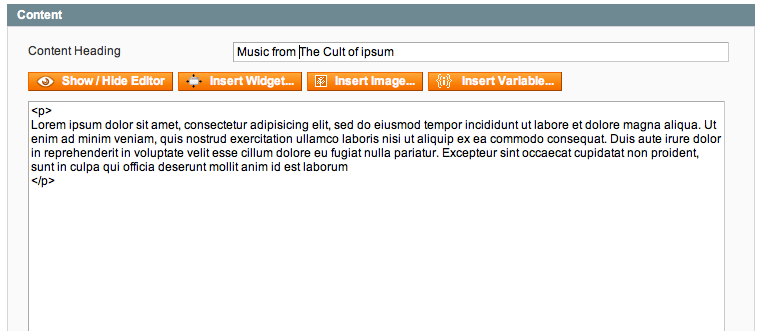
\includegraphics[width=1\textwidth]{images/chapter7/show-hide.png}
\end{center}
\caption{}
%\label{fig:awesome_image}
\end{figure}


The WYSIWYG editing will disappear and be replaced by an HTML source editor.  More importantly, you'll have a new list of buttons, one of which is \textbf{Insert Widget}.  Click on this button, and a modal window will come up (see \emph{Figure 7.2})

\begin{figure}[htb]
\begin{center}
\leavevmode
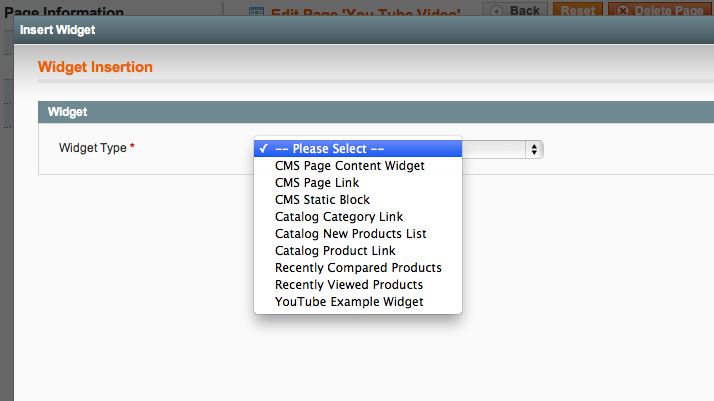
\includegraphics[width=1\textwidth]{images/chapter7/widget-window.png}
\end{center}
\caption{}
%\label{fig:awesome_image}
\end{figure}


If you click on the \textbf{Widget Type} drop-down, you'll see a list of standard Magento widgets, with your \textbf{YouTube Example Widget} widget listed last.

Select your widget from the menu and click in \textbf{Insert Widget}.  You should notice the following text has been added to your HTML source

\begin{lstlisting}
{{widget type="nofrills_booklayout/youtube"}}

\end{lstlisting}


Save your CMS page, and then load the page

\begin{lstlisting}
http://magento.example.com/example-youtube

\end{lstlisting}


in a your web browser.   You should see your embedded YouTube video.

\section{CMS Template Directives}

The \footnotesize\texttt{\{\{curly braces\}\}} \normalsize  text is a template directive.  When Magento encounters these, a template engine will kick in.  If your widget isn't displaying correctly and you want to debug this template engine, hop to the following file

\begin{lstlisting}
#File: app/code/core/Mage/Widget/Model/Template/Filter.php
...
class Mage_Widget_Model_Template_Filter extends Mage_Cms_Model_Template_Filter
{
    ...
    public function widgetDirective($construction)
    {
        ...widget directives are rendered here...
    }
    ...
}

\end{lstlisting}


Every directive in a CMS page works this way.  Just look for the method name that matches the directive name, followed by the word directive.

\begin{lstlisting}
widgetDirective
templateDirective
foobazbarDirective

\end{lstlisting}


The \footnotesize\texttt{\{\{widget\}\}} \normalsize  directive has a useful feature. You can use it to set properties on your widget block object (see Appendix G: Magento Magic setters and getters).  We can use this to make our widget a bit more useful.

Change your block code so it matches the following, and refresh the CMS page.

\begin{lstlisting}
<?php
class Nofrills_Booklayout_Block_Youtube extends Mage_Core_Block_Abstract
implements Mage_Widget_Block_Interface
{
    protected function _toHtml()
    {
        $this->setVideoId('dQw4w9WgXcQ');
        return '
            <object width="640" height="505">
                <param name="movie" value="http://www.youtube.com/v/' .
                $this->getVideoId() .
                '?fs=1&amp;hl=en_US"></param>
                <param name="allowFullScreen" value="true"></param>
                <param name="allowscriptaccess" value="always"></param>
                <embed src="http://www.youtube.com/v/' .
                $this->getVideoId() .
                '?fs=1&amp;hl=en_US"
                type="application/x-shockwave-flash" allowscriptaccess="always" ' .
                'allowfullscreen="true" width="640" height="505"></embed>
            </object>
        ';
    }
}

\end{lstlisting}


Your CMS page will remain unchanged.  We've altered the code above to set a \footnotesize\texttt{video\_id} \normalsize  data property on the block object, and then used that property in rendering the YouTube embed code. (Remember, data properties are stored with underscore\_notation, but the magic methods to fetch them are CamelCased)

Next, remove the following line from your block and reload the CMS page.

\begin{lstlisting}
$this->setVideoId('dQw4w9WgXcQ');

\end{lstlisting}


Without setting this property, the video will fail to render.  So far that's all pretty obvious.  Next, edit the widget directive so it looks like the following

\begin{lstlisting}
{{widget type="nofrills_booklayout/youtube" video_id="dQw4w9WgXcQ"}}

\end{lstlisting}


Save the CMS page, and reload the frontend page in your browser.  Your video is back!

The \footnotesize\texttt{widgetDirective} \normalsize  method will parse the directive text for attributes, and if it finds any they'll be assigned as data attributes to the widget object.  With this feature, your widgets go from static content renderers to dynamic content renderers.

\section{Adding Data Property UI}

Of course, the whole point of widgets is that they're meant as a method of code-less block adding.  While it's good to \textbf{know} you can edit the widget directives directly, something more is needed if this feature is going to fulfill its promise.

In your widget config, add a \footnotesize\texttt{\textless parameters/\textgreater } \normalsize  node as defined below.

\begin{lstlisting}
<!-- #File: app/code/local/Nofrills/Booklayout/etc/widget.xml -->
<widgets>
    <nofrills_layoutbook_youtube type="nofrills_booklayout/youtube">
        <name>YouTube Example Widget</name>
        <description type="desc">
            This wiget displays a YouTube video.
        </description>

        <!-- START new section -->
        <parameters>
            <video_id>
                <required>1</required>
                <visible>1</visible>
                <value>Enter ID Here</value>
                <label>YouTube Video ID</label>
                <type>text</type>
            </video_id>
        </parameters>
        <!-- END new section -->

    </nofrills_layoutbook_youtube>
</widgets>

\end{lstlisting}


Clear your cache, and then click on the \textbf{Insert Widget} button again.  Select your widget from the drop-down, and you will now see a UI for entering a video ID, (see \emph{Figure 7.3})

\begin{figure}[htb]
\begin{center}
\leavevmode
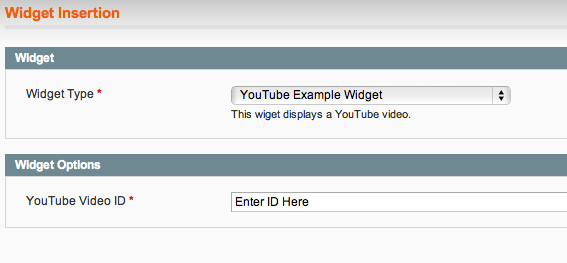
\includegraphics[width=1\textwidth]{images/chapter7/widget-window-with-data.png}
\end{center}
\caption{}
%\label{fig:awesome_image}
\end{figure}


Enter an ID (we recommend \footnotesize\texttt{qYkbTyHXwbs} \normalsize  to keep with the theme) and click on \textbf{Insert Widget}.  The following directive code should be inserted into the content area.

\begin{lstlisting}
{{widget type="nofrills_booklayout/youtube" video_id="qYkbTyHXwbs"}}

\end{lstlisting}


Easy as that, you now have a widget for inserting any YouTube video into any page.  Let's take a look at the XML we added to our widget config

\begin{lstlisting}
<parameters>
    <video_id>
        <required>1</required>
        <visible>1</visible>
        <value>Enter ID Here</value>
        <label>YouTube Video ID</label>
        <type>text</type>
    </video_id>
</parameters>

\end{lstlisting}


This node will \emph{formally} add data parameters to our widget, and allow us to specify a field type for data entry.  The \footnotesize\texttt{\textless video\_id\textgreater } \normalsize  tag here \textbf{does have} semantic value, it's the name of the attribute that will be added to the directive tag

\begin{lstlisting}
{{widget type="nofrills_booklayout/youtube" video_id="[VALUE]"}}

\end{lstlisting}


The \footnotesize\texttt{\textless required\textgreater } \normalsize  tag allows a level of data validation, setting this to "1" will force the Admin Console user to enter a value before inserting the widget.

The \footnotesize\texttt{\textless visible/\textgreater } \normalsize  node allows you to hide the input field for this data parameter, and have the inserted widget directive tag automatically include an attribute every time its used, with a value provided by the \footnotesize\texttt{\textless value/\textgreater } \normalsize  tag.  When \footnotesize\texttt{\textless visible/\textgreater } \normalsize  is set to 1 the \footnotesize\texttt{\textless value/\textgreater } \normalsize  tag will be used as a default ID.

The value in \footnotesize\texttt{\textless label\textgreater } \normalsize  will be used to provide your rendered HTML form with a label, and \footnotesize\texttt{\textless type/\textgreater } \normalsize  controls what sort of form element is rendered.  See Appendix G for a full list and explanation of form rendering configurations.

\textbf{Important}: Be careful changing data parameters of a deployed widget.  Once a \footnotesize\texttt{\{\{widget...\}\}} \normalsize  directive tag has been added to a CMS page, it become "detached" from its definition.  That is, if we changed the \footnotesize\texttt{\textless video\_id/\textgreater } \normalsize  above to be \footnotesize\texttt{\textless youtube\_id/\textgreater }\normalsize, our CMS page would still have the

\begin{lstlisting}
{{widget type="nofrills_booklayout/youtube" video_id="[VALUE]"}}

\end{lstlisting}


widget tag.  While this isn't necessarily a problem, it may cause confusion while further developing the widget or debugging rendering issues.

\section{Widget Templates}

Looking back at our five defining widget properties

\begin{enumerate}
\item Widgets are Magento Template Blocks
\item Widgets Contain Structured Data
\item Widgets Contain Rules for Building User Interfaces
\item Widgets are formally associated with a number of phtml template files
\item Widgets contain rules that say which blocks in the layout system are allowed to contain them
\end{enumerate}


we can see that we've covered 1 - 3.  Next up is widget templates.

Just like an ordinary block, a widget can be rendered using a phtml template.  Additionally, using the UI rendering features, we can make templates a \textbf{customizable} feature of our widget.

Let's make our YouTube widget a template block.  First, we'll alter our class so it inherits from the core template block and we'll remove the hard coded \footnotesize\texttt{\_toHtml} \normalsize  method.

\begin{lstlisting}
#File: app/code/local/Nofrills/Booklayout/Block/Youtube.php
<?php
class Nofrills_Booklayout_Block_Youtube extends Mage_Core_Block_Template
implements Mage_Widget_Block_Interface
{

}

\end{lstlisting}


Next, we'll add the following parameter to our widget config

\begin{lstlisting}
<parameters>
    <!-- ... -->
    <template>
        <required>1</required>
        <visible>0</visible>
        <value>youtube.phtml</value>
        <label>Frontend Template</label>
        <type>text</type>
    </template>
    <!-- ... -->
</parameters>

\end{lstlisting}


Finally, we'll add the \footnotesize\texttt{youtube.phtml} \normalsize  to our theme's template folder.  We're adding it to the default/default theme here, but if your site's using a different theme, make sure you put it in the appropriate location

\begin{lstlisting}
<!-- #File: app/design/frontend/default/default/template/youtube.phtml -->
<h2>Rick</h2>
<object width="640" height="505">
    <param name="movie" value="http://www.youtube.com/v/'<?php
    echo $this->getVideoId();?>?fs=1&amp;hl=en_US"></param>
    <param name="allowFullScreen" value="true"></param>
    <param name="allowscriptaccess" value="always"></param>
    <embed src="http://www.youtube.com/v/<?php
    echo $this->getVideoId();?>?fs=1&amp;hl=en_US"
    type="application/x-shockwave-flash" allowscriptaccess="always"
    allowfullscreen="true" width="640" height="505"></embed>
</object>

\end{lstlisting}


With all of the above in place (and a cache clear), re-insert your widget.  You should get a widget tag with a template attribute

\begin{lstlisting}
{{widget type="nofrills_booklayout/youtube" video_id="qYkbTyHXwbs"
template="youtube.phtml"}}

\end{lstlisting}


Reload your frontend page and your configured YouTube video should render the same as before.

Because template blocks store their template as a regular block data parameter, all we're really doing here is adding a new widget data parameter named \footnotesize\texttt{\textless template/\textgreater }\normalsize.  We hard coded a value (by using an invisible data field), but there's no reason we couldn't make it a truly configurable value.  Give the following a try in your widget config

\begin{lstlisting}
<template>
    <required>1</required>
    <visible>1</visible>
    <value>youtube.phtml</value>
    <label>Frontend Template</label>
    <type>select</type>

    <values>
        <as_video>
            <value>youtube.phtml</value>
            <label>Embed Video</label>
        </as_video>
        <as_link>
            <value>youtube-as-link.phtml</value>
            <label>Link Video</label>
        </as_link>
    </values>
</template>

\end{lstlisting}


Don't forget to add the new template to your theme

\begin{lstlisting}
<?php
#File: app/design/frontend/default/default/template/youtube-as-link.phtml
?>
<a href="http://www.youtube.com/watch?v=<?php
    echo $this->getVideoId();?>">Watch this!?</a>

\end{lstlisting}


Clear your cache and reinsert your widget.  You should now see a new drop-down menu allowing you to pick which template your widget should use, (see \emph{Figure 7.4})

\begin{figure}[htb]
\begin{center}
\leavevmode
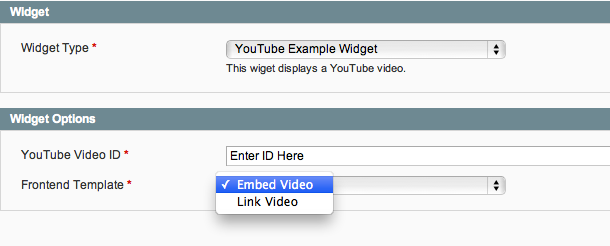
\includegraphics[width=1\textwidth]{images/chapter7/with-template.png}
\end{center}
\caption{}
%\label{fig:awesome_image}
\end{figure}


While it may appear that the template tag is being treated as just another widget property, when we move outside of CMS based widgets and into Instance Widgets, we'll see that the Instance Widget engine treats this parameter specially.

\section{Instance Widgets}

If we look back on our list of five things that make a widget

\begin{enumerate}
\item Widgets are Magento Template Blocks
\item Widgets Contain Structured Data
\item Widgets Contain Rules for Building User Interfaces
\item Widgets are formally associated with a number of phtml template files
\item Widgets contain rules that say which blocks in the layout system are allowed to contain them
\end{enumerate}


we can see our explorations have completely ignored number five.  So far all we've done is insert a widget into a CMS content area.  We also haven't met our core widget requirement, which is to allow a non-programming user to add a widget to \textbf{any} page on the site. This is where Instance Widgets enter the picture.

So far we've been creating one off widgets that can't be reused.  For example, if we wanted to add the same video to multiple CMS pages, we'd need to manually insert it into each page.  Then, if we wanted to \textbf{change} something about each widget (say, the ID of that video), we'd need to go to each individual page and edit the template directive tag

\begin{lstlisting}
{{widget type="nofrills_booklayout/youtube" video_id="dQw4w9WgXcQ"}}

\end{lstlisting}


With Instance Widgets, we can create \textbf{and save} a widget with a specific set of data, and then insert that widget into multiple locations on the site.  Then, if we later change the definition of that specific widget, it will be automatically updated throughout the site.

\section{Creating an Instance Widget}

Navigate to

\begin{lstlisting}
CMS -> Widgets

\end{lstlisting}


in the Admin Console to see a list of all the widgets in your system.  We're going to add a new one, so click on the \textbf{Add New Widget Instance} button

Instance Widget creation is a two step process.  First, we need to select the widget type we're going to create, as well as which theme the widget will be added to.  Select our \textbf{YouTube} example widget from the drop down menu, and pick the currently configured theme.  We'll be assuming \footnotesize\texttt{default/default} \normalsize  for the following examples, (see \emph{Figure 7.5})

\begin{figure}[htb]
\begin{center}
\leavevmode
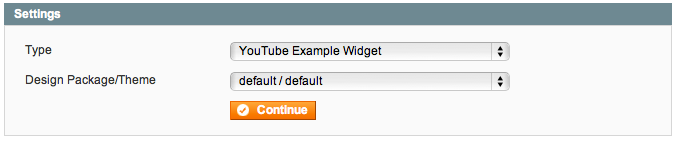
\includegraphics[width=1\textwidth]{images/chapter7/instance-step1.png}
\end{center}
\caption{}
%\label{fig:awesome_image}
\end{figure}


Once you've done this, click on the \textbf{Continue} button.

You should now see a two tab editing interface; \textbf{Frontend Properties}, and \textbf{Widget Options}.    Widget Options contains an editing form for all the data properties for a particular widget, (with the exception of templates).  Click on this tab and add a video id, and then return to the Frontend Properties tab, (see \emph{Figure 7.6})

\begin{figure}[htb]
\begin{center}
\leavevmode
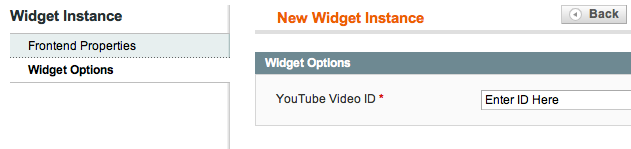
\includegraphics[width=1\textwidth]{images/chapter7/instance-set-data.png}
\end{center}
\caption{}
%\label{fig:awesome_image}
\end{figure}


In Frontend Properties you have two option groups.  The first allows you to select a Widget Instance Title, Assign a Store View, and set a Sort Order for the widget.  The Widget Instance Title is used in the Admin Console when displaying information about the widget (i.e. the listing page), Store View allows you to specify which Magento Stores a widget appears in.

Let's save our widget with a title, and select \emph{All Store Views}.  Click on the \textbf{Save} button, and you'll be returned to the widget listing page.  You should see your widget listed along with any others that have been added to your Magento system.  Click on the widget row to edit it.  You'll notice you've been brought directly to the second stage, and that the \textbf{Widget Type} and \textbf{Design Package/Theme} options are un-editable. Once you select these during widget creation they \textbf{cannot} be changed, (see \emph{Figure 7.7})

\begin{figure}[htb]
\begin{center}
\leavevmode
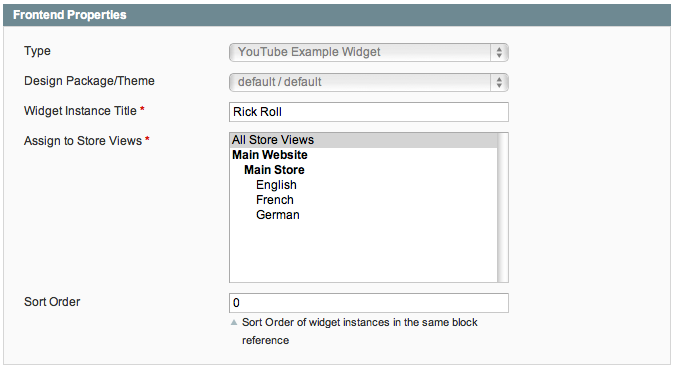
\includegraphics[width=1\textwidth]{images/chapter7/instance-step2-always.png}
\end{center}
\caption{}
%\label{fig:awesome_image}
\end{figure}


\section{Inserting a Widget}

Here's where Instance Widgets get interesting. At the bottom of the Instance Widget editing page, there's an empty option group named \textbf{Layout Update}.  Click the \textbf{Add Layout Update} button, (see \emph{Figure 7.8})

\begin{figure}[htb]
\begin{center}
\leavevmode
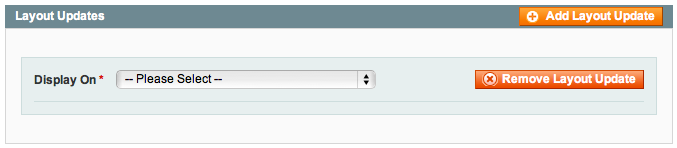
\includegraphics[width=1\textwidth]{images/chapter7/instance-displayon.png}
\end{center}
\caption{}
%\label{fig:awesome_image}
\end{figure}


This drop down menu contains several options, each one describing a particular set of, or a specific, Magento page.  What we're configuring here is the page or pages we want to add our Widget Instance to.  Select All Pages from this menu, (see \emph{Figure 7.9})

\begin{figure}[htb]
\begin{center}
\leavevmode
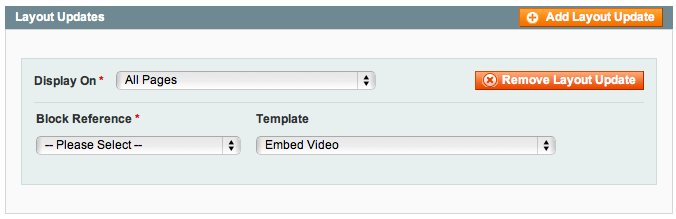
\includegraphics[width=1\textwidth]{images/chapter7/instance-pageselected.png}
\end{center}
\caption{}
%\label{fig:awesome_image}
\end{figure}


Two more menus have appeared.  The first is \textbf{Block Reference}, the second is \textbf{Template}.

The first menu is defining \textbf{which block} you want to add your Widget Instance to.  Select \textbf{Main Content Area}.  The values in the second menu should look familiar to you.  They're the templates we defined earlier.  Select "Embed Video", and then Save you Widget Instance.

At this point you may receive a message at the top of your Magento admin that looks something like \emph{Figure 7.10}.

\begin{figure}[htb]
\begin{center}
\leavevmode
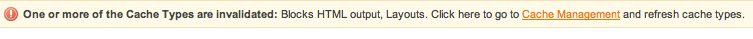
\includegraphics[width=1\textwidth]{images/chapter7/invalidated.png}
\end{center}
\caption{}
%\label{fig:awesome_image}
\end{figure}


This is Magento telling you that it has detected a change to the system that requires you to clear your cache.  Do this, and then load any page in your site.  You should now see your YouTube video added to the main content area.

\section{Behind the Scenes}

Open up your favorite MySQL browser, and run the following query against your database

\begin{lstlisting}
select * from core_layout_update;
+------------------+----------------------+---------+------------+
| layout_update_id | handle               | xml     | sort_order |
+------------------+----------------------+----------------------+
|                1 | default              | [...]   |          0 |
+------------------+----------------------+----------------------+

\end{lstlisting}


This table contains a list of Layout Update XML fragments, organized by handle.  When building the Page Layout for any request, Magento will check this table \textbf{after} checking the loaded package layout.  If it finds any matching handles, they'll be added to the Page Layout.  When you select a value from the \textbf{Display On} menu, you're actually telling Magento \textbf{which} handles should be applied.  When you save your Widget Instance, this table is updated.  Because these updates add blocks to other block's that inherit from \footnotesize\texttt{core/text\_list}\normalsize, the widget blocks are automatically rendered.

If you take a look at the \footnotesize\texttt{Mage\_Core\_Model\_Layout\_Update::merge} \normalsize  method, you can see the additional call to \footnotesize\texttt{fetchDbLayoutUpdates} \normalsize

\begin{lstlisting}
public function merge($handle)
{
    $packageUpdatesStatus = $this->fetchPackageLayoutUpdates($handle);
    if (Mage::app()->isInstalled()) {
        $this->fetchDbLayoutUpdates($handle);
    }
    return $this;
}

\end{lstlisting}


Without an abstract Layout system, adding a feature like widgets would have required (at minimum) editing every single controller action, and inserting blocks into an unknown layout structure. This is the kind of power that sort of abstraction enables.

Similarly, the list of blocks which you insert a widget into is \textbf{not} hardcoded into a configuration system.  It's generated automatically.  Magento takes the handle indicated by the \textbf{Display On} drop down, and applies it to the Package Layout to create a temporary Page Layout.  Then, rather than render a page, it looks at the top level body blocks for that layout to get a list of eligible blocks to display in the drop-down menu.  This means if you add additional structural blocks to a page via means of custom XML layout files or \footnotesize\texttt{local.xml}\normalsize, those blocks will show up in this menu.  Again, this sort of thing becomes much easier to implement when using an abstract layout system.

\section{Restricting Blocks.}

Widget Instances have one more interesting feature.  You can actually restrict \textbf{which} blocks a Widget Instance may be inserted into.  Head back to your \footnotesize\texttt{widget.xml} \normalsize  file, and add the following to  your widget's node

\begin{lstlisting}
<widgets>
    <nofrills_layoutbook_youtube>
        <!-- ... -->
        <supported_blocks>
            <uniquely_named_node>
                <block_name>content</block_name>
                <template>
                    <unique_name_one>as_video</unique_name_one>
                    <unique_name_two>as_link</unique_name_two>
                </template>
            </uniquely_named_node>

            <another_uniquely_named_node>
                <block_name>left</block_name>
                <template>
                    <unique_name_one>as_video</unique_name_one>
                    <unique_name_two>as_link</unique_name_two>
                </template>
            </another_uniquely_named_node>

        </supported_blocks>
        <!-- ... -->
    </nofrills_layoutbook_youtube>
</widgets>

\end{lstlisting}


Clear your cache and reload the Widget Instance editing page.  Your (formerly) long block menu now only allows you the choice of

\begin{lstlisting}
Left Column
Main Content Area

\end{lstlisting}


In the absence of a \footnotesize\texttt{\textless supported\_blocks/\textgreater } \normalsize  tag, Magento will display all eligible blocks for any particular page.  However, with this node in place, it will scan each top level node for a sub-node named \footnotesize\texttt{\textless block\_name\textgreater } \normalsize  and restrict your choices to those it finds.  In our case above, the blocks are \footnotesize\texttt{content} \normalsize  and \footnotesize\texttt{left}\normalsize.  These names are the block's name as defined in the Layout Update XML fragment

\begin{lstlisting}
<block type="core/text_list" name="content" as="content" translate="label">

\end{lstlisting}


You're also required to specify which, if any, templates are valid for a particular block.  This context sensitive template is a powerful feature.  Consider and add the following change to your \footnotesize\texttt{widget.xml} \normalsize  file

\begin{lstlisting}
<uniquely_named_node>
    <block_name>content</block_name>
    <template>
        <unique_name_one>as_video</unique_name_one>
        <unique_name_two>as_link</unique_name_two>
    </template>
</uniquely_named_node>

<another_uniquely_named_node>
    <block_name>left</block_name>
    <template>
        <unique_name_two>as_link</unique_name_two>
    </template>
</another_uniquely_named_node>

\end{lstlisting}


Clear your cache and reload the widget editor.  You'll notice that switching between the \footnotesize\texttt{content} \normalsize  and \footnotesize\texttt{left} \normalsize  block will result in your template choice being restricted.  By using this technique, we've prevented a user from accidentally inserting a full video into the left hand column by restricting the templates they can use.  In essence, each widget definition is an abstract content type, and you can control how it displays in each section of the site.  This is only a few steps away from some of the advanced content management features of systems like Drupal.

The values being supplied for the templates (\footnotesize\texttt{as\_link} \normalsize  and \footnotesize\texttt{as\_video}\normalsize) are the names of the nodes in the \footnotesize\texttt{<templates/>} \normalsize  block up in the \footnotesize\texttt{\textless parameters/\textgreater } \normalsize  section.  This is what we've meant when we said Magento treats this node differently.

\section{Per Theme Widget Config}

There's another feature of the widget engine, in relation to Instances, that you should be aware of.  It's possible to create fall back configurations for your widgets on a \textbf{per theme} basis.  You've probably noticed the default themes each ship with a widget file.

\begin{lstlisting}
app/design/frontend/default/default/etc/widget.xml

\end{lstlisting}


This file has the same format as the \footnotesize\texttt{widget.xml} \normalsize  in your module.  Values in these files can be used to \textbf{override} the values for Instance Widgets.  They \textbf{do not} apply to widgets inserted into CMS Pages or Static Blocks.  In practice, this is done primarily for the supported blocks feature.   Keeping with the generate principle of separating concerns, a general code module doesn't, technically, know which blocks or templates are going to be available for it.  By keeping this information in each theme (Magento's default widgets ship with all the \footnotesize\texttt{\textless supported\_blocks/\textgreater } \normalsize  information in the theme configs), Magento ensures that any themes which add custom \footnotesize\texttt{core/text\_list} \normalsize  blocks also have the ability to allow or deny widgets access to these blocks.

\section{Wrap Up}

And that, in a nutshell, is widgets.  We chose to end this book with widgets, because they appear to be the path forward for Magento content and layout management.  The abstract layout system described in this book is stepping stone towards larger, more robust content and layout management for Magento.  Less than four years old, Magento is dominating the ecommerce landscape like no other system. We hope the knowedge and techniques provided here will help you tame your Magento systems, and allow you to spend less time being confused by code, and more time serving your customers and building your businesses.

\emph{Visit http://www.pulsestorm.net/nofrills-layout-chapter-seven to join the discussion online.}
\appendix
\chapter{Magento Block Hierarchy}
This tree is a directory style hierarchy of every block class in Magento CE 1.4.2.0.

\begin{lstlisting}
`-- Varien_Object
|-- Mage_Core_Block_Abstract
|   |-- Mage_Adminhtml_Block_Urlrewrite_Link
|   |-- Mage_CatalogSearch_Block_Autocomplete
|   |-- Mage_Catalog_Block_Product_Price_Template
|   |-- Mage_Cms_Block_Block
|   |-- Mage_Cms_Block_Page
|   |-- Mage_Core_Block_Flush
|   |-- Mage_Core_Block_Html_Select
|   |   |-- Mage_Adminhtml_Block_Html_Select
|   |   `-- Mage_CatalogInventory_Block_Adminhtml_Form_Field_Customergroup
|   |-- Mage_Core_Block_Html_Select
|   |-- Mage_Core_Block_Profiler
|   |-- Mage_Core_Block_Template
|   |   |-- Mage_Adminhtml_Block_Abstract
|   |   |   |-- Mage_Adminhtml_Block_Catalog_Product_Frontend_Product_Watermark
|   |   |   |-- Mage_Adminhtml_Block_Customer_Edit_Renderer_Newpass
|   |   |   |-- Mage_Adminhtml_Block_Customer_Edit_Renderer_Region
|   |   |   |-- Mage_Adminhtml_Block_Extensions_Custom_Edit_Tab_Load
|   |   |   |-- Mage_Adminhtml_Block_Promo_Widget_Chooser_Daterange
|   |   |   |-- Mage_Adminhtml_Block_System_Config_Form_Field
|   |   |   |   |-- Mage_Adminhtml_Block_Catalog_Form_Renderer_Config_DateFieldsOrder
|   |   |   |   |-- Mage_Adminhtml_Block_Catalog_Form_Renderer_Config_YearRange
|   |   |   |   |-- Mage_Adminhtml_Block_Report_Config_Form_Field_MtdStart
|   |   |   |   |-- Mage_Adminhtml_Block_Report_Config_Form_Field_YtdStart
|   |   |   |   |-- Mage_Adminhtml_Block_System_Config_Form_Field_Array_Abstract
|   |   |   |   |   |-- Mage_Adminhtml_Block_System_Config_Form_Field_Regexceptions
|   |   |   |   |   `-- Mage_CatalogInventory_Block_Adminhtml_Form_Field_Minsaleqty
|   |   |   |   |-- Mage_Adminhtml_Block_System_Config_Form_Field_Array_Abstract
|   |   |   |   |-- Mage_Adminhtml_Block_System_Config_Form_Field_Datetime
|   |   |   |   |-- Mage_Adminhtml_Block_System_Config_Form_Field_Notification
|   |   |   |   |-- Mage_Adminhtml_Block_System_Config_Form_Field_Select_Flatcatalog
|   |   |   |   |-- Mage_Adminhtml_Block_System_Config_Form_Field_Select_Flatproduct
|   |   |   |   |-- Mage_Directory_Block_Adminhtml_Frontend_Currency_Base
|   |   |   |   |-- Mage_Directory_Block_Adminhtml_Frontend_Region_Updater
|   |   |   |   |-- Mage_GoogleCheckout_Block_Adminhtml_Shipping_Applicable_Countries
|   |   |   |   |-- Mage_GoogleCheckout_Block_Adminhtml_Shipping_Merchant
|   |   |   |   |-- Mage_Paypal_Block_Adminhtml_System_Config_ApiWizard
|   |   |   |   `-- Mage_Tax_Block_Adminhtml_Frontend_Region_Updater
|   |   |   |-- Mage_Adminhtml_Block_System_Config_Form_Field
|   |   |   |-- Mage_Adminhtml_Block_System_Config_Form_Field_Heading
|   |   |   |-- Mage_Adminhtml_Block_System_Config_Form_Fieldset
|   |   |   |   |-- Mage_Adminhtml_Block_System_Config_Form_Fieldset_Modules_DisableOutput
|   |   |   |   `-- Mage_Adminhtml_Block_System_Config_Form_Fieldset_Order_Statuses
|   |   |   |-- Mage_Adminhtml_Block_System_Config_Form_Fieldset
|   |   |   |-- Mage_Adminhtml_Block_System_Convert_Profile_Run
|   |   |   |-- Mage_Adminhtml_Block_Widget_Form_Element_Dependence
|   |   |   |-- Mage_Adminhtml_Block_Widget_Grid_Column_Filter_Abstract
|   |   |   |   |-- Mage_Adminhtml_Block_Newsletter_Problem_Grid_Filter_Checkbox
|   |   |   |   |-- Mage_Adminhtml_Block_Newsletter_Subscriber_Grid_Filter_Checkbox
|   |   |   |   |-- Mage_Adminhtml_Block_System_Convert_Profile_Edit_Filter_Action
|   |   |   |   |-- Mage_Adminhtml_Block_Widget_Grid_Column_Filter_Date
|   |   |   |   |   `-- Mage_Adminhtml_Block_Widget_Grid_Column_Filter_Datetime
|   |   |   |   |-- Mage_Adminhtml_Block_Widget_Grid_Column_Filter_Date
|   |   |   |   |-- Mage_Adminhtml_Block_Widget_Grid_Column_Filter_Price
|   |   |   |   |-- Mage_Adminhtml_Block_Widget_Grid_Column_Filter_Range
|   |   |   |   |-- Mage_Adminhtml_Block_Widget_Grid_Column_Filter_Select
|   |   |   |   |   |-- Mage_Adminhtml_Block_Catalog_Product_Edit_Tab_Super_Config_Grid_Filter_Inventory
|   |   |   |   |   |-- Mage_Adminhtml_Block_Customer_Edit_Tab_Newsletter_Grid_Filter_Status
|   |   |   |   |   |-- Mage_Adminhtml_Block_Customer_Grid_Filter_Country
|   |   |   |   |   |-- Mage_Adminhtml_Block_Newsletter_Subscriber_Grid_Filter_Website
|   |   |   |   |   |-- Mage_Adminhtml_Block_Review_Grid_Filter_Type
|   |   |   |   |   |-- Mage_Adminhtml_Block_System_Email_Template_Grid_Filter_Type
|   |   |   |   |   |-- Mage_Adminhtml_Block_Widget_Grid_Column_Filter_Checkbox
|   |   |   |   |   |   `-- Mage_Adminhtml_Block_Widget_Grid_Column_Filter_Massaction
|   |   |   |   |   |-- Mage_Adminhtml_Block_Widget_Grid_Column_Filter_Checkbox
|   |   |   |   |   |-- Mage_Adminhtml_Block_Widget_Grid_Column_Filter_Country
|   |   |   |   |   `-- Mage_Adminhtml_Block_Widget_Grid_Column_Filter_Radio
|   |   |   |   |-- Mage_Adminhtml_Block_Widget_Grid_Column_Filter_Select
|   |   |   |   |-- Mage_Adminhtml_Block_Widget_Grid_Column_Filter_Store
|   |   |   |   |-- Mage_Adminhtml_Block_Widget_Grid_Column_Filter_Text
|   |   |   |   `-- Mage_Adminhtml_Block_Widget_Grid_Column_Filter_Theme
|   |   |   |-- Mage_Adminhtml_Block_Widget_Grid_Column_Filter_Abstract
|   |   |   |-- Mage_Adminhtml_Block_Widget_Grid_Column_Renderer_Abstract
|   |   |   |   |-- Mage_Adminhtml_Block_Catalog_Product_Edit_Tab_Super_Config_Grid_Renderer_Inventory
|   |   |   |   |-- Mage_Adminhtml_Block_Cms_Page_Grid_Renderer_Action
|   |   |   |   |-- Mage_Adminhtml_Block_Customer_Edit_Tab_Newsletter_Grid_Renderer_Action
|   |   |   |   |-- Mage_Adminhtml_Block_Customer_Edit_Tab_Newsletter_Grid_Renderer_Status
|   |   |   |   |-- Mage_Adminhtml_Block_Customer_Edit_Tab_Wishlist_Grid_Renderer_Description
|   |   |   |   |-- Mage_Adminhtml_Block_Customer_Online_Grid_Renderer_Ip
|   |   |   |   |-- Mage_Adminhtml_Block_Customer_Online_Grid_Renderer_Type
|   |   |   |   |-- Mage_Adminhtml_Block_Customer_Online_Grid_Renderer_Url
|   |   |   |   |-- Mage_Adminhtml_Block_Dashboard_Searches_Renderer_Searchquery
|   |   |   |   |-- Mage_Adminhtml_Block_Newsletter_Problem_Grid_Renderer_Checkbox
|   |   |   |   |-- Mage_Adminhtml_Block_Newsletter_Subscriber_Grid_Renderer_Checkbox
|   |   |   |   |-- Mage_Adminhtml_Block_Newsletter_Template_Grid_Renderer_Sender
|   |   |   |   |-- Mage_Adminhtml_Block_Notification_Grid_Renderer_Actions
|   |   |   |   |-- Mage_Adminhtml_Block_Notification_Grid_Renderer_Notice
|   |   |   |   |-- Mage_Adminhtml_Block_Notification_Grid_Renderer_Severity
|   |   |   |   |-- Mage_Adminhtml_Block_Report_Grid_Column_Renderer_Customer
|   |   |   |   |-- Mage_Adminhtml_Block_Report_Grid_Column_Renderer_Product
|   |   |   |   |-- Mage_Adminhtml_Block_Report_Product_Downloads_Renderer_Purchases
|   |   |   |   |-- Mage_Adminhtml_Block_Review_Grid_Renderer_Type
|   |   |   |   |-- Mage_Adminhtml_Block_Sales_Reorder_Renderer_Action
|   |   |   |   |-- Mage_Adminhtml_Block_Sitemap_Grid_Renderer_Link
|   |   |   |   |-- Mage_Adminhtml_Block_Sitemap_Grid_Renderer_Time
|   |   |   |   |-- Mage_Adminhtml_Block_System_Convert_Profile_Edit_Renderer_Action
|   |   |   |   |-- Mage_Adminhtml_Block_System_Email_Template_Grid_Renderer_Sender
|   |   |   |   |-- Mage_Adminhtml_Block_System_Email_Template_Grid_Renderer_Type
|   |   |   |   |-- Mage_Adminhtml_Block_System_Store_Grid_Render_Group
|   |   |   |   |-- Mage_Adminhtml_Block_System_Store_Grid_Render_Store
|   |   |   |   |-- Mage_Adminhtml_Block_System_Store_Grid_Render_Website
|   |   |   |   |-- Mage_Adminhtml_Block_Tax_Rate_Grid_Renderer_Data
|   |   |   |   |-- Mage_Adminhtml_Block_Widget_Grid_Column_Renderer_Checkbox
|   |   |   |   |   |-- Mage_Adminhtml_Block_Catalog_Product_Edit_Tab_Super_Config_Grid_Renderer_Checkbox
|   |   |   |   |   |-- Mage_Adminhtml_Block_Sales_Order_Create_Search_Grid_Renderer_Giftmessage
|   |   |   |   |   `-- Mage_Adminhtml_Block_Widget_Grid_Column_Renderer_Massaction
|   |   |   |   |-- Mage_Adminhtml_Block_Widget_Grid_Column_Renderer_Checkbox
|   |   |   |   |-- Mage_Adminhtml_Block_Widget_Grid_Column_Renderer_Concat
|   |   |   |   |-- Mage_Adminhtml_Block_Widget_Grid_Column_Renderer_Country
|   |   |   |   |   `-- Mage_Adminhtml_Block_Tax_Rate_Grid_Renderer_Country
|   |   |   |   |-- Mage_Adminhtml_Block_Widget_Grid_Column_Renderer_Country
|   |   |   |   |-- Mage_Adminhtml_Block_Widget_Grid_Column_Renderer_Currency
|   |   |   |   |   `-- Mage_Adminhtml_Block_Report_Grid_Column_Renderer_Currency
|   |   |   |   |-- Mage_Adminhtml_Block_Widget_Grid_Column_Renderer_Currency
|   |   |   |   |-- Mage_Adminhtml_Block_Widget_Grid_Column_Renderer_Date
|   |   |   |   |   `-- Mage_Adminhtml_Block_Report_Sales_Grid_Column_Renderer_Date
|   |   |   |   |-- Mage_Adminhtml_Block_Widget_Grid_Column_Renderer_Date
|   |   |   |   |-- Mage_Adminhtml_Block_Widget_Grid_Column_Renderer_Datetime
|   |   |   |   |-- Mage_Adminhtml_Block_Widget_Grid_Column_Renderer_Input
|   |   |   |   |-- Mage_Adminhtml_Block_Widget_Grid_Column_Renderer_Ip
|   |   |   |   |-- Mage_Adminhtml_Block_Widget_Grid_Column_Renderer_Longtext
|   |   |   |   |-- Mage_Adminhtml_Block_Widget_Grid_Column_Renderer_Number
|   |   |   |   |   `-- Mage_Adminhtml_Block_Report_Grid_Column_Renderer_Blanknumber
|   |   |   |   |-- Mage_Adminhtml_Block_Widget_Grid_Column_Renderer_Number
|   |   |   |   |-- Mage_Adminhtml_Block_Widget_Grid_Column_Renderer_Price
|   |   |   |   |   `-- Mage_Adminhtml_Block_Sales_Order_Create_Search_Grid_Renderer_Price
|   |   |   |   |-- Mage_Adminhtml_Block_Widget_Grid_Column_Renderer_Price
|   |   |   |   |-- Mage_Adminhtml_Block_Widget_Grid_Column_Renderer_Radio
|   |   |   |   |-- Mage_Adminhtml_Block_Widget_Grid_Column_Renderer_Select
|   |   |   |   |-- Mage_Adminhtml_Block_Widget_Grid_Column_Renderer_Store
|   |   |   |   |-- Mage_Adminhtml_Block_Widget_Grid_Column_Renderer_Text
|   |   |   |   |   |-- Mage_Adminhtml_Block_Widget_Grid_Column_Renderer_Action
|   |   |   |   |   |   |-- Mage_Adminhtml_Block_Extensions_Local_Grid_Renderer_Action
|   |   |   |   |   |   |-- Mage_Adminhtml_Block_Extensions_Remote_Grid_Renderer_Action
|   |   |   |   |   |   |-- Mage_Adminhtml_Block_Newsletter_Queue_Grid_Renderer_Action
|   |   |   |   |   |   |-- Mage_Adminhtml_Block_Newsletter_Template_Grid_Renderer_Action
|   |   |   |   |   |   |-- Mage_Adminhtml_Block_Sitemap_Grid_Renderer_Action
|   |   |   |   |   |   `-- Mage_Adminhtml_Block_System_Email_Template_Grid_Renderer_Action
|   |   |   |   |   |-- Mage_Adminhtml_Block_Widget_Grid_Column_Renderer_Action
|   |   |   |   |   `-- Mage_Adminhtml_Block_Widget_Grid_Column_Renderer_Options
|   |   |   |   |-- Mage_Adminhtml_Block_Widget_Grid_Column_Renderer_Text
|   |   |   |   |-- Mage_Adminhtml_Block_Widget_Grid_Column_Renderer_Theme
|   |   |   |   |-- Mage_Adminhtml_Block_Widget_Grid_Column_Renderer_Wrapline
|   |   |   |   |-- Mage_GoogleBase_Block_Adminhtml_Items_Renderer_Id
|   |   |   |   `-- Mage_GoogleBase_Block_Adminhtml_Types_Renderer_Country
|   |   |   |-- Mage_Adminhtml_Block_Widget_Grid_Column_Renderer_Abstract
|   |   |   |-- Mage_Paypal_Block_Adminhtml_System_Config_Fieldset_Global
|   |   |   |-- Mage_Paypal_Block_Adminhtml_System_Config_Fieldset_Hint
|   |   |   |-- Mage_Sales_Block_Adminhtml_Billing_Agreement_View_Tab_Info
|   |   |   `-- Mage_Sales_Block_Adminhtml_Recurring_Profile_Edit_Form
|   |   |-- Mage_Adminhtml_Block_Abstract
|   |   |-- Mage_Adminhtml_Block_Catalog_Product_Edit_Tab_Ajax_Serializer
|   |   |-- Mage_Adminhtml_Block_Sales_Order_Create_Load
|   |   |-- Mage_Adminhtml_Block_Tax_Rate_Title
|   |   |-- Mage_Adminhtml_Block_Template
|   |   |   |-- Mage_Adminhtml_Block_Api_Buttons
|   |   |   |-- Mage_Adminhtml_Block_Api_Roles
|   |   |   |-- Mage_Adminhtml_Block_Api_Users
|   |   |   |-- Mage_Adminhtml_Block_Backup
|   |   |   |-- Mage_Adminhtml_Block_Cache_Additional
|   |   |   |-- Mage_Adminhtml_Block_Cache_Notifications
|   |   |   |-- Mage_Adminhtml_Block_Catalog
|   |   |   |-- Mage_Adminhtml_Block_Catalog_Category_Abstract
|   |   |   |   |-- Mage_Adminhtml_Block_Catalog_Category_Edit_Form
|   |   |   |   |-- Mage_Adminhtml_Block_Catalog_Category_Tree
|   |   |   |   |   |-- Mage_Adminhtml_Block_Catalog_Category_Checkboxes_Tree
|   |   |   |   |   |-- Mage_Adminhtml_Block_Catalog_Category_Widget_Chooser
|   |   |   |   |   `-- Mage_Adminhtml_Block_Catalog_Product_Edit_Tab_Categories
|   |   |   |   |-- Mage_Adminhtml_Block_Catalog_Category_Tree
|   |   |   |   `-- Mage_Adminhtml_Block_Urlrewrite_Category_Tree
|   |   |   |-- Mage_Adminhtml_Block_Catalog_Category_Abstract
|   |   |   |-- Mage_Adminhtml_Block_Catalog_Product_Attribute_Set_Main
|   |   |   |-- Mage_Adminhtml_Block_Catalog_Product_Attribute_Set_Main_Tree_Attribute
|   |   |   |-- Mage_Adminhtml_Block_Catalog_Product_Attribute_Set_Main_Tree_Group
|   |   |   |-- Mage_Adminhtml_Block_Catalog_Product_Attribute_Set_Toolbar_Add
|   |   |   |-- Mage_Adminhtml_Block_Catalog_Product_Attribute_Set_Toolbar_Main
|   |   |   |-- Mage_Adminhtml_Block_Catalog_Product_Edit_Js
|   |   |   |-- Mage_Adminhtml_Block_Catalog_Product_Edit_Tab_Alerts
|   |   |   |-- Mage_Adminhtml_Block_Catalog_Product_Widget_Chooser_Container
|   |   |   |-- Mage_Adminhtml_Block_Cms_Wysiwyg_Images_Content_Files
|   |   |   |-- Mage_Adminhtml_Block_Cms_Wysiwyg_Images_Content_Newfolder
|   |   |   |-- Mage_Adminhtml_Block_Cms_Wysiwyg_Images_Tree
|   |   |   |-- Mage_Adminhtml_Block_Customer_Edit_Tab_Carts
|   |   |   |-- Mage_Adminhtml_Block_Customer_Edit_Tab_View
|   |   |   |-- Mage_Adminhtml_Block_Customer_Edit_Tab_View_Sales
|   |   |   |-- Mage_Adminhtml_Block_Customer_Online
|   |   |   |-- Mage_Adminhtml_Block_Dashboard
|   |   |   |-- Mage_Adminhtml_Block_Denied
|   |   |   |-- Mage_Adminhtml_Block_Newsletter_Problem
|   |   |   |-- Mage_Adminhtml_Block_Newsletter_Queue
|   |   |   |-- Mage_Adminhtml_Block_Newsletter_Queue_Edit
|   |   |   |-- Mage_Adminhtml_Block_Newsletter_Subscriber
|   |   |   |-- Mage_Adminhtml_Block_Newsletter_Template
|   |   |   |-- Mage_Adminhtml_Block_Notification_Baseurl
|   |   |   |-- Mage_Adminhtml_Block_Notification_Security
|   |   |   |-- Mage_Adminhtml_Block_Notification_Survey
|   |   |   |-- Mage_Adminhtml_Block_Notification_Toolbar
|   |   |   |   `-- Mage_Adminhtml_Block_Notification_Window
|   |   |   |-- Mage_Adminhtml_Block_Notification_Toolbar
|   |   |   |-- Mage_Adminhtml_Block_Page
|   |   |   |-- Mage_Adminhtml_Block_Page_Footer
|   |   |   |-- Mage_Adminhtml_Block_Page_Header
|   |   |   |-- Mage_Adminhtml_Block_Page_Menu
|   |   |   |-- Mage_Adminhtml_Block_Page_Notices
|   |   |   |-- Mage_Adminhtml_Block_Permissions_Buttons
|   |   |   |-- Mage_Adminhtml_Block_Permissions_Roles
|   |   |   |-- Mage_Adminhtml_Block_Permissions_Usernroles
|   |   |   |-- Mage_Adminhtml_Block_Permissions_Users
|   |   |   |-- Mage_Adminhtml_Block_Poll_Edit_Tab_Answers_List
|   |   |   |-- Mage_Adminhtml_Block_Report_Wishlist
|   |   |   |-- Mage_Adminhtml_Block_Review_Rating_Detailed
|   |   |   |-- Mage_Adminhtml_Block_Review_Rating_Summary
|   |   |   |-- Mage_Adminhtml_Block_Sales
|   |   |   |-- Mage_Adminhtml_Block_Sales_Items_Abstract
|   |   |   |   |-- Mage_Adminhtml_Block_Sales_Items_Renderer_Configurable
|   |   |   |   |-- Mage_Adminhtml_Block_Sales_Items_Renderer_Default
|   |   |   |   |   `-- Mage_Bundle_Block_Adminhtml_Sales_Order_Items_Renderer
|   |   |   |   |-- Mage_Adminhtml_Block_Sales_Items_Renderer_Default
|   |   |   |   |-- Mage_Adminhtml_Block_Sales_Order_Creditmemo_Create_Items
|   |   |   |   |-- Mage_Adminhtml_Block_Sales_Order_Creditmemo_View_Items
|   |   |   |   |-- Mage_Adminhtml_Block_Sales_Order_Invoice_Create_Items
|   |   |   |   |-- Mage_Adminhtml_Block_Sales_Order_Invoice_View_Items
|   |   |   |   |-- Mage_Adminhtml_Block_Sales_Order_Shipment_Create_Items
|   |   |   |   |-- Mage_Adminhtml_Block_Sales_Order_Shipment_View_Items
|   |   |   |   |-- Mage_Adminhtml_Block_Sales_Order_View_Items
|   |   |   |   |-- Mage_Adminhtml_Block_Sales_Order_View_Items_Renderer_Default
|   |   |   |   |   `-- Mage_Bundle_Block_Adminhtml_Sales_Order_View_Items_Renderer
|   |   |   |   `-- Mage_Adminhtml_Block_Sales_Order_View_Items_Renderer_Default
|   |   |   |-- Mage_Adminhtml_Block_Sales_Items_Abstract
|   |   |   |-- Mage_Adminhtml_Block_Sales_Items_Column_Default
|   |   |   |   |-- Mage_Adminhtml_Block_Sales_Items_Column_Name
|   |   |   |   |   |-- Mage_Adminhtml_Block_Sales_Items_Column_Name_Grouped
|   |   |   |   |   `-- Mage_Downloadable_Block_Adminhtml_Sales_Items_Column_Downloadable_Name
|   |   |   |   |-- Mage_Adminhtml_Block_Sales_Items_Column_Name
|   |   |   |   `-- Mage_Adminhtml_Block_Sales_Items_Column_Qty
|   |   |   |-- Mage_Adminhtml_Block_Sales_Items_Column_Default
|   |   |   |-- Mage_Adminhtml_Block_Sales_Order_Comments_View
|   |   |   |-- Mage_Adminhtml_Block_Sales_Order_Create_Totals_Table
|   |   |   |-- Mage_Adminhtml_Block_Sales_Order_Creditmemo_Create_Adjustments
|   |   |   |-- Mage_Adminhtml_Block_Sales_Order_Invoice_Create_Tracking
|   |   |   |-- Mage_Adminhtml_Block_Sales_Order_Payment
|   |   |   |-- Mage_Adminhtml_Block_Sales_Order_Shipment_Create_Tracking
|   |   |   |-- Mage_Adminhtml_Block_Sales_Order_Shipment_Tracking_Info
|   |   |   |-- Mage_Adminhtml_Block_Sales_Order_Shipment_View_Tracking
|   |   |   |-- Mage_Adminhtml_Block_Sales_Order_View_Form
|   |   |   |-- Mage_Adminhtml_Block_Sales_Order_View_History
|   |   |   |-- Mage_Adminhtml_Block_Sales_Order_View_Tab_History
|   |   |   |-- Mage_Adminhtml_Block_Store_Switcher
|   |   |   |   |-- Mage_Adminhtml_Block_Catalog_Product_Edit_Tab_Websites
|   |   |   |   |-- Mage_Adminhtml_Block_Sales_Order_Create_Store_Select
|   |   |   |   |-- Mage_Adminhtml_Block_Tag_Store_Switcher
|   |   |   |   `-- Mage_GoogleBase_Block_Adminhtml_Store_Switcher
|   |   |   |-- Mage_Adminhtml_Block_Store_Switcher
|   |   |   |-- Mage_Adminhtml_Block_System_Config_Switcher
|   |   |   |-- Mage_Adminhtml_Block_System_Convert_Profile_Edit_Tab_Run
|   |   |   |-- Mage_Adminhtml_Block_System_Currency
|   |   |   |-- Mage_Adminhtml_Block_System_Currency_Rate_Matrix
|   |   |   |-- Mage_Adminhtml_Block_System_Currency_Rate_Services
|   |   |   |-- Mage_Adminhtml_Block_System_Design
|   |   |   |-- Mage_Adminhtml_Block_System_Email_Template
|   |   |   |-- Mage_Adminhtml_Block_System_Store_Delete_Group
|   |   |   |-- Mage_Adminhtml_Block_System_Store_Delete_Website
|   |   |   |-- Mage_Adminhtml_Block_Tag
|   |   |   |-- Mage_Adminhtml_Block_Tag_Pending
|   |   |   |-- Mage_Adminhtml_Block_Tax_Rate_Toolbar_Add
|   |   |   |-- Mage_Adminhtml_Block_Tax_Rate_Toolbar_Save
|   |   |   |-- Mage_Adminhtml_Block_Widget
|   |   |   |   |-- Mage_Adminhtml_Block_Catalog_Product_Attribute_New_Product_Created
|   |   |   |   |-- Mage_Adminhtml_Block_Catalog_Product_Created
|   |   |   |   |-- Mage_Adminhtml_Block_Catalog_Product_Edit
|   |   |   |   |-- Mage_Adminhtml_Block_Catalog_Product_Edit_Action_Attribute
|   |   |   |   |-- Mage_Adminhtml_Block_Catalog_Product_Edit_Action_Attribute_Tab_Inventory
|   |   |   |   |-- Mage_Adminhtml_Block_Catalog_Product_Edit_Action_Attribute_Tab_Websites
|   |   |   |   |-- Mage_Adminhtml_Block_Catalog_Product_Edit_Tab_Inventory
|   |   |   |   |-- Mage_Adminhtml_Block_Catalog_Product_Edit_Tab_Options
|   |   |   |   |-- Mage_Adminhtml_Block_Catalog_Product_Edit_Tab_Options_Option
|   |   |   |   |-- Mage_Adminhtml_Block_Catalog_Product_Edit_Tab_Options_Type_Abstract
|   |   |   |   |-- Mage_Adminhtml_Block_Catalog_Product_Edit_Tab_Price_Tier
|   |   |   |   |-- Mage_Adminhtml_Block_Catalog_Product_Edit_Tab_Super_Config
|   |   |   |   |-- Mage_Adminhtml_Block_Catalog_Product_Helper_Form_Gallery_Content
|   |   |   |   |-- Mage_Adminhtml_Block_Dashboard_Abstract
|   |   |   |   |   |-- Mage_Adminhtml_Block_Dashboard_Bar
|   |   |   |   |   |   |-- Mage_Adminhtml_Block_Dashboard_Sales
|   |   |   |   |   |   `-- Mage_Adminhtml_Block_Dashboard_Totals
|   |   |   |   |   |-- Mage_Adminhtml_Block_Dashboard_Bar
|   |   |   |   |   |-- Mage_Adminhtml_Block_Dashboard_Graph
|   |   |   |   |   |   |-- Mage_Adminhtml_Block_Dashboard_Tab_Amounts
|   |   |   |   |   |   `-- Mage_Adminhtml_Block_Dashboard_Tab_Orders
|   |   |   |   |   `-- Mage_Adminhtml_Block_Dashboard_Graph
|   |   |   |   |-- Mage_Adminhtml_Block_Dashboard_Abstract
|   |   |   |   |-- Mage_Adminhtml_Block_Extensions_Config_Edit
|   |   |   |   |-- Mage_Adminhtml_Block_Media_Editor
|   |   |   |   |-- Mage_Adminhtml_Block_Media_Uploader
|   |   |   |   |   `-- Mage_Adminhtml_Block_Cms_Wysiwyg_Images_Content_Uploader
|   |   |   |   |-- Mage_Adminhtml_Block_Media_Uploader
|   |   |   |   |-- Mage_Adminhtml_Block_Newsletter_Queue_Preview
|   |   |   |   |-- Mage_Adminhtml_Block_Newsletter_Template_Edit
|   |   |   |   |-- Mage_Adminhtml_Block_Newsletter_Template_Preview
|   |   |   |   |-- Mage_Adminhtml_Block_Sales_Order_Abstract
|   |   |   |   |   |-- Mage_Adminhtml_Block_Sales_Order_Creditmemo_Create_Form
|   |   |   |   |   |-- Mage_Adminhtml_Block_Sales_Order_Creditmemo_View_Form
|   |   |   |   |   |-- Mage_Adminhtml_Block_Sales_Order_Invoice_Create_Form
|   |   |   |   |   |-- Mage_Adminhtml_Block_Sales_Order_Invoice_View_Form
|   |   |   |   |   |-- Mage_Adminhtml_Block_Sales_Order_Shipment_Create_Form
|   |   |   |   |   |-- Mage_Adminhtml_Block_Sales_Order_Shipment_View_Form
|   |   |   |   |   |-- Mage_Adminhtml_Block_Sales_Order_Totalbar
|   |   |   |   |   |-- Mage_Adminhtml_Block_Sales_Order_View_Info
|   |   |   |   |   `-- Mage_Adminhtml_Block_Sales_Order_View_Tab_Info
|   |   |   |   |-- Mage_Adminhtml_Block_Sales_Order_Abstract
|   |   |   |   |-- Mage_Adminhtml_Block_Sales_Order_Create_Abstract
|   |   |   |   |   |-- Mage_Adminhtml_Block_Sales_Order_Create_Billing_Method
|   |   |   |   |   |-- Mage_Adminhtml_Block_Sales_Order_Create_Comment
|   |   |   |   |   |-- Mage_Adminhtml_Block_Sales_Order_Create_Coupons
|   |   |   |   |   |-- Mage_Adminhtml_Block_Sales_Order_Create_Coupons_Form
|   |   |   |   |   |-- Mage_Adminhtml_Block_Sales_Order_Create_Customer
|   |   |   |   |   |-- Mage_Adminhtml_Block_Sales_Order_Create_Data
|   |   |   |   |   |-- Mage_Adminhtml_Block_Sales_Order_Create_Form
|   |   |   |   |   |-- Mage_Adminhtml_Block_Sales_Order_Create_Form_Abstract
|   |   |   |   |   |   |-- Mage_Adminhtml_Block_Sales_Order_Create_Form_Account
|   |   |   |   |   |   |-- Mage_Adminhtml_Block_Sales_Order_Create_Form_Address
|   |   |   |   |   |   |   |-- Mage_Adminhtml_Block_Sales_Order_Create_Billing_Address
|   |   |   |   |   |   |   `-- Mage_Adminhtml_Block_Sales_Order_Create_Shipping_Address
|   |   |   |   |   |   `-- Mage_Adminhtml_Block_Sales_Order_Create_Form_Address
|   |   |   |   |   |-- Mage_Adminhtml_Block_Sales_Order_Create_Form_Abstract
|   |   |   |   |   |-- Mage_Adminhtml_Block_Sales_Order_Create_Giftmessage
|   |   |   |   |   |-- Mage_Adminhtml_Block_Sales_Order_Create_Header
|   |   |   |   |   |-- Mage_Adminhtml_Block_Sales_Order_Create_Items
|   |   |   |   |   |-- Mage_Adminhtml_Block_Sales_Order_Create_Items_Grid
|   |   |   |   |   |-- Mage_Adminhtml_Block_Sales_Order_Create_Newsletter
|   |   |   |   |   |-- Mage_Adminhtml_Block_Sales_Order_Create_Search
|   |   |   |   |   |-- Mage_Adminhtml_Block_Sales_Order_Create_Shipping_Method
|   |   |   |   |   |-- Mage_Adminhtml_Block_Sales_Order_Create_Shipping_Method_Form
|   |   |   |   |   |-- Mage_Adminhtml_Block_Sales_Order_Create_Sidebar
|   |   |   |   |   |-- Mage_Adminhtml_Block_Sales_Order_Create_Sidebar_Abstract
|   |   |   |   |   |   |-- Mage_Adminhtml_Block_Sales_Order_Create_Sidebar_Cart
|   |   |   |   |   |   |-- Mage_Adminhtml_Block_Sales_Order_Create_Sidebar_Compared
|   |   |   |   |   |   |-- Mage_Adminhtml_Block_Sales_Order_Create_Sidebar_Pcompared
|   |   |   |   |   |   |-- Mage_Adminhtml_Block_Sales_Order_Create_Sidebar_Pviewed
|   |   |   |   |   |   |-- Mage_Adminhtml_Block_Sales_Order_Create_Sidebar_Reorder
|   |   |   |   |   |   |-- Mage_Adminhtml_Block_Sales_Order_Create_Sidebar_Viewed
|   |   |   |   |   |   `-- Mage_Adminhtml_Block_Sales_Order_Create_Sidebar_Wishlist
|   |   |   |   |   |-- Mage_Adminhtml_Block_Sales_Order_Create_Sidebar_Abstract
|   |   |   |   |   |-- Mage_Adminhtml_Block_Sales_Order_Create_Store
|   |   |   |   |   |-- Mage_Adminhtml_Block_Sales_Order_Create_Totals
|   |   |   |   |   |   |-- Mage_Adminhtml_Block_Sales_Order_Create_Totals_Default
|   |   |   |   |   |   |   |-- Mage_Adminhtml_Block_Sales_Order_Create_Totals_Discount
|   |   |   |   |   |   |   |-- Mage_Adminhtml_Block_Sales_Order_Create_Totals_Grandtotal
|   |   |   |   |   |   |   |-- Mage_Adminhtml_Block_Sales_Order_Create_Totals_Shipping
|   |   |   |   |   |   |   |-- Mage_Adminhtml_Block_Sales_Order_Create_Totals_Subtotal
|   |   |   |   |   |   |   `-- Mage_Adminhtml_Block_Sales_Order_Create_Totals_Tax
|   |   |   |   |   |   `-- Mage_Adminhtml_Block_Sales_Order_Create_Totals_Default
|   |   |   |   |   |-- Mage_Adminhtml_Block_Sales_Order_Create_Totals
|   |   |   |   |   |-- Mage_Centinel_Block_Adminhtml_Validation
|   |   |   |   |   `-- Mage_Centinel_Block_Adminhtml_Validation_Form
|   |   |   |   |-- Mage_Adminhtml_Block_Sales_Order_Create_Abstract
|   |   |   |   |-- Mage_Adminhtml_Block_Sales_Order_Create_Newsletter_Form
|   |   |   |   |-- Mage_Adminhtml_Block_Sales_Order_View_Giftmessage
|   |   |   |   |-- Mage_Adminhtml_Block_System_Cache_Edit
|   |   |   |   |-- Mage_Adminhtml_Block_System_Config_Edit
|   |   |   |   |-- Mage_Adminhtml_Block_System_Config_Tabs
|   |   |   |   |-- Mage_Adminhtml_Block_System_Design_Edit
|   |   |   |   |-- Mage_Adminhtml_Block_System_Email_Template_Edit
|   |   |   |   |-- Mage_Adminhtml_Block_System_Email_Template_Preview
|   |   |   |   |-- Mage_Adminhtml_Block_Tax_Rate_ImportExport
|   |   |   |   |-- Mage_Adminhtml_Block_Widget_Accordion
|   |   |   |   |   |-- Mage_Adminhtml_Block_Customer_Edit_Tab_View_Accordion
|   |   |   |   |   |-- Mage_Adminhtml_Block_Tag_Edit_Accordion
|   |   |   |   |   `-- Mage_Adminhtml_Block_Tag_Edit_Assigned
|   |   |   |   |-- Mage_Adminhtml_Block_Widget_Accordion
|   |   |   |   |-- Mage_Adminhtml_Block_Widget_Accordion_Item
|   |   |   |   |-- Mage_Adminhtml_Block_Widget_Button
|   |   |   |   |   `-- Mage_Adminhtml_Block_Catalog_Product_Edit_Tab_Attributes_Create
|   |   |   |   |-- Mage_Adminhtml_Block_Widget_Button
|   |   |   |   |-- Mage_Adminhtml_Block_Widget_Form
|   |   |   |   |   |-- Find_Feed_Block_Adminhtml_Edit_Codes_Edit_Form
|   |   |   |   |   |-- Mage_Adminhtml_Block_Api_Tab_Roleinfo
|   |   |   |   |   |-- Mage_Adminhtml_Block_Api_Tab_Rolesedit
|   |   |   |   |   |-- Mage_Adminhtml_Block_Api_User_Edit_Form
|   |   |   |   |   |-- Mage_Adminhtml_Block_Api_User_Edit_Tab_Main
|   |   |   |   |   |-- Mage_Adminhtml_Block_Catalog_Form
|   |   |   |   |   |   |-- Mage_Adminhtml_Block_Catalog_Category_Tab_Attributes
|   |   |   |   |   |   |-- Mage_Adminhtml_Block_Catalog_Category_Tab_Design
|   |   |   |   |   |   |-- Mage_Adminhtml_Block_Catalog_Category_Tab_General
|   |   |   |   |   |   |-- Mage_Adminhtml_Block_Catalog_Product_Attribute_New_Product_Attributes
|   |   |   |   |   |   |-- Mage_Adminhtml_Block_Catalog_Product_Edit_Action_Attribute_Tab_Attributes
|   |   |   |   |   |   |-- Mage_Adminhtml_Block_Catalog_Product_Edit_Tab_Attributes
|   |   |   |   |   |   |   |-- Mage_Adminhtml_Block_Catalog_Product_Edit_Tab_Super_Config_Simple
|   |   |   |   |   |   |   `-- Mage_Bundle_Block_Adminhtml_Catalog_Product_Edit_Tab_Attributes
|   |   |   |   |   |   |-- Mage_Adminhtml_Block_Catalog_Product_Edit_Tab_Attributes
|   |   |   |   |   |   |-- Mage_GoogleOptimizer_Block_Adminhtml_Catalog_Category_Edit_Tab_Googleoptimizer
|   |   |   |   |   |   `-- Mage_GoogleOptimizer_Block_Adminhtml_Catalog_Product_Edit_Tab_Googleoptimizer
|   |   |   |   |   |-- Mage_Adminhtml_Block_Catalog_Form
|   |   |   |   |   |-- Mage_Adminhtml_Block_Catalog_Helper_Form_Wysiwyg_Content
|   |   |   |   |   |-- Mage_Adminhtml_Block_Catalog_Product_Attribute_Edit_Form
|   |   |   |   |   |-- Mage_Adminhtml_Block_Catalog_Product_Attribute_Edit_Tab_Front
|   |   |   |   |   |-- Mage_Adminhtml_Block_Catalog_Product_Attribute_Edit_Tab_System
|   |   |   |   |   |-- Mage_Adminhtml_Block_Catalog_Product_Attribute_Set_Main_Formattribute
|   |   |   |   |   |-- Mage_Adminhtml_Block_Catalog_Product_Attribute_Set_Main_Formgroup
|   |   |   |   |   |-- Mage_Adminhtml_Block_Catalog_Product_Attribute_Set_Main_Formset
|   |   |   |   |   |-- Mage_Adminhtml_Block_Catalog_Product_Attribute_Set_Toolbar_Main_Filter
|   |   |   |   |   |-- Mage_Adminhtml_Block_Catalog_Product_Edit_Tab_Price
|   |   |   |   |   |-- Mage_Adminhtml_Block_Catalog_Product_Edit_Tab_Settings
|   |   |   |   |   |-- Mage_Adminhtml_Block_Catalog_Product_Edit_Tab_Super_Settings
|   |   |   |   |   |-- Mage_Adminhtml_Block_Catalog_Search_Edit_Form
|   |   |   |   |   |-- Mage_Adminhtml_Block_Checkout_Agreement_Edit_Form
|   |   |   |   |   |-- Mage_Adminhtml_Block_Cms_Block_Edit_Form
|   |   |   |   |   |-- Mage_Adminhtml_Block_Cms_Page_Edit_Form
|   |   |   |   |   |-- Mage_Adminhtml_Block_Cms_Page_Edit_Tab_Content
|   |   |   |   |   |-- Mage_Adminhtml_Block_Cms_Page_Edit_Tab_Design
|   |   |   |   |   |-- Mage_Adminhtml_Block_Cms_Page_Edit_Tab_Main
|   |   |   |   |   |-- Mage_Adminhtml_Block_Cms_Page_Edit_Tab_Meta
|   |   |   |   |   |-- Mage_Adminhtml_Block_Customer_Edit_Form
|   |   |   |   |   |-- Mage_Adminhtml_Block_Customer_Edit_Tab_Account
|   |   |   |   |   |-- Mage_Adminhtml_Block_Customer_Edit_Tab_Addresses
|   |   |   |   |   |-- Mage_Adminhtml_Block_Customer_Edit_Tab_Newsletter
|   |   |   |   |   |-- Mage_Adminhtml_Block_Customer_Group_Edit_Form
|   |   |   |   |   |-- Mage_Adminhtml_Block_Customer_Online_Filter
|   |   |   |   |   |-- Mage_Adminhtml_Block_Extensions_Config_Form
|   |   |   |   |   |-- Mage_Adminhtml_Block_Extensions_Console_Edit_Form
|   |   |   |   |   |-- Mage_Adminhtml_Block_Extensions_Custom_Edit_Form
|   |   |   |   |   |-- Mage_Adminhtml_Block_Extensions_Custom_Edit_Tab_Abstract
|   |   |   |   |   |   |-- Mage_Adminhtml_Block_Extensions_Custom_Edit_Tab_Contents
|   |   |   |   |   |   |-- Mage_Adminhtml_Block_Extensions_Custom_Edit_Tab_Depends
|   |   |   |   |   |   |-- Mage_Adminhtml_Block_Extensions_Custom_Edit_Tab_Maintainers
|   |   |   |   |   |   |-- Mage_Adminhtml_Block_Extensions_Custom_Edit_Tab_Package
|   |   |   |   |   |   `-- Mage_Adminhtml_Block_Extensions_Custom_Edit_Tab_Release
|   |   |   |   |   |-- Mage_Adminhtml_Block_Extensions_Custom_Edit_Tab_Abstract
|   |   |   |   |   |-- Mage_Adminhtml_Block_Extensions_File_Form
|   |   |   |   |   |-- Mage_Adminhtml_Block_Extensions_Local_Edit_Form
|   |   |   |   |   |-- Mage_Adminhtml_Block_Extensions_Local_Edit_Tab_Abstract
|   |   |   |   |   |   |-- Mage_Adminhtml_Block_Extensions_Local_Edit_Tab_Actions
|   |   |   |   |   |   |-- Mage_Adminhtml_Block_Extensions_Local_Edit_Tab_Changelog
|   |   |   |   |   |   |-- Mage_Adminhtml_Block_Extensions_Local_Edit_Tab_Contents
|   |   |   |   |   |   |-- Mage_Adminhtml_Block_Extensions_Local_Edit_Tab_Depends
|   |   |   |   |   |   `-- Mage_Adminhtml_Block_Extensions_Local_Edit_Tab_Package
|   |   |   |   |   |-- Mage_Adminhtml_Block_Extensions_Local_Edit_Tab_Abstract
|   |   |   |   |   |-- Mage_Adminhtml_Block_Extensions_Local_Upgrade
|   |   |   |   |   |-- Mage_Adminhtml_Block_Extensions_Mass_Install
|   |   |   |   |   |-- Mage_Adminhtml_Block_Extensions_Mass_Uninstall
|   |   |   |   |   |-- Mage_Adminhtml_Block_Extensions_Mass_Upgrade
|   |   |   |   |   |-- Mage_Adminhtml_Block_Extensions_Remote_Edit_Form
|   |   |   |   |   |-- Mage_Adminhtml_Block_Extensions_Remote_Edit_Tab_Abstract
|   |   |   |   |   |   |-- Mage_Adminhtml_Block_Extensions_Remote_Edit_Tab_Actions
|   |   |   |   |   |   |-- Mage_Adminhtml_Block_Extensions_Remote_Edit_Tab_Changelog
|   |   |   |   |   |   `-- Mage_Adminhtml_Block_Extensions_Remote_Edit_Tab_Package
|   |   |   |   |   |-- Mage_Adminhtml_Block_Extensions_Remote_Edit_Tab_Abstract
|   |   |   |   |   |-- Mage_Adminhtml_Block_Newsletter_Queue_Edit_Form
|   |   |   |   |   |-- Mage_Adminhtml_Block_Newsletter_Template_Edit_Form
|   |   |   |   |   |-- Mage_Adminhtml_Block_Newsletter_Template_Preview_Form
|   |   |   |   |   |-- Mage_Adminhtml_Block_Permissions_Tab_Roleinfo
|   |   |   |   |   |-- Mage_Adminhtml_Block_Permissions_Tab_Rolesedit
|   |   |   |   |   |-- Mage_Adminhtml_Block_Permissions_Tab_Useredit
|   |   |   |   |   |-- Mage_Adminhtml_Block_Permissions_User_Edit_Form
|   |   |   |   |   |-- Mage_Adminhtml_Block_Permissions_User_Edit_Tab_Main
|   |   |   |   |   |-- Mage_Adminhtml_Block_Poll_Answer_Edit_Form
|   |   |   |   |   |-- Mage_Adminhtml_Block_Poll_Edit_Form
|   |   |   |   |   |-- Mage_Adminhtml_Block_Poll_Edit_Tab_Answers_Form
|   |   |   |   |   |-- Mage_Adminhtml_Block_Poll_Edit_Tab_Form
|   |   |   |   |   |-- Mage_Adminhtml_Block_Promo_Catalog_Edit_Form
|   |   |   |   |   |-- Mage_Adminhtml_Block_Promo_Catalog_Edit_Tab_Actions
|   |   |   |   |   |-- Mage_Adminhtml_Block_Promo_Catalog_Edit_Tab_Conditions
|   |   |   |   |   |-- Mage_Adminhtml_Block_Promo_Catalog_Edit_Tab_Main
|   |   |   |   |   |-- Mage_Adminhtml_Block_Promo_Quote_Edit_Form
|   |   |   |   |   |-- Mage_Adminhtml_Block_Promo_Quote_Edit_Tab_Actions
|   |   |   |   |   |-- Mage_Adminhtml_Block_Promo_Quote_Edit_Tab_Conditions
|   |   |   |   |   |-- Mage_Adminhtml_Block_Promo_Quote_Edit_Tab_Labels
|   |   |   |   |   |-- Mage_Adminhtml_Block_Promo_Quote_Edit_Tab_Main
|   |   |   |   |   |-- Mage_Adminhtml_Block_Rating_Edit_Form
|   |   |   |   |   |-- Mage_Adminhtml_Block_Rating_Edit_Tab_Form
|   |   |   |   |   |-- Mage_Adminhtml_Block_Rating_Edit_Tab_Options
|   |   |   |   |   |-- Mage_Adminhtml_Block_Report_Filter_Form
|   |   |   |   |   |   |-- Mage_Sales_Block_Adminhtml_Report_Filter_Form
|   |   |   |   |   |   |   `-- Mage_Sales_Block_Adminhtml_Report_Filter_Form_Order
|   |   |   |   |   |   `-- Mage_Sales_Block_Adminhtml_Report_Filter_Form
|   |   |   |   |   |-- Mage_Adminhtml_Block_Report_Filter_Form
|   |   |   |   |   |-- Mage_Adminhtml_Block_Review_Add_Form
|   |   |   |   |   |-- Mage_Adminhtml_Block_Review_Edit_Form
|   |   |   |   |   |-- Mage_Adminhtml_Block_Sales_Order_Create_Giftmessage_Form
|   |   |   |   |   |-- Mage_Adminhtml_Block_Sitemap_Edit_Form
|   |   |   |   |   |-- Mage_Adminhtml_Block_System_Account_Edit_Form
|   |   |   |   |   |-- Mage_Adminhtml_Block_System_Cache_Form
|   |   |   |   |   |-- Mage_Adminhtml_Block_System_Config_Form
|   |   |   |   |   |-- Mage_Adminhtml_Block_System_Convert_Gui_Edit_Form
|   |   |   |   |   |-- Mage_Adminhtml_Block_System_Convert_Gui_Edit_Tab_Upload
|   |   |   |   |   |-- Mage_Adminhtml_Block_System_Convert_Gui_Edit_Tab_View
|   |   |   |   |   |-- Mage_Adminhtml_Block_System_Convert_Profile_Edit_Form
|   |   |   |   |   |-- Mage_Adminhtml_Block_System_Convert_Profile_Edit_Tab_Edit
|   |   |   |   |   |-- Mage_Adminhtml_Block_System_Currency_Edit_Form
|   |   |   |   |   |-- Mage_Adminhtml_Block_System_Currency_Edit_Tab_Main
|   |   |   |   |   |-- Mage_Adminhtml_Block_System_Currency_Edit_Tab_Rates
|   |   |   |   |   |-- Mage_Adminhtml_Block_System_Design_Edit_Tab_General
|   |   |   |   |   |-- Mage_Adminhtml_Block_System_Email_Template_Edit_Form
|   |   |   |   |   |-- Mage_Adminhtml_Block_System_Store_Delete_Form
|   |   |   |   |   |-- Mage_Adminhtml_Block_System_Store_Edit_Form
|   |   |   |   |   |-- Mage_Adminhtml_Block_System_Variable_Edit_Form
|   |   |   |   |   |-- Mage_Adminhtml_Block_Tag_Edit_Form
|   |   |   |   |   |-- Mage_Adminhtml_Block_Tag_Tag_Edit_Form
|   |   |   |   |   |-- Mage_Adminhtml_Block_Tax_Class_Edit_Form
|   |   |   |   |   |-- Mage_Adminhtml_Block_Tax_Rate_Form
|   |   |   |   |   |-- Mage_Adminhtml_Block_Tax_Rule_Edit_Form
|   |   |   |   |   |-- Mage_Adminhtml_Block_Urlrewrite_Edit_Form
|   |   |   |   |   |-- Mage_Adminhtml_Block_Widget_Grid_Massaction_Item_Additional_Default
|   |   |   |   |   |-- Mage_Eav_Block_Adminhtml_Attribute_Edit_Main_Abstract
|   |   |   |   |   |   `-- Mage_Adminhtml_Block_Catalog_Product_Attribute_Edit_Tab_Main
|   |   |   |   |   |-- Mage_Eav_Block_Adminhtml_Attribute_Edit_Main_Abstract
|   |   |   |   |   |-- Mage_GoogleBase_Block_Adminhtml_Types_Edit_Form
|   |   |   |   |   |-- Mage_GoogleOptimizer_Block_Adminhtml_Cms_Page_Edit_Tab_Googleoptimizer
|   |   |   |   |   |-- Mage_Index_Block_Adminhtml_Process_Edit_Form
|   |   |   |   |   |-- Mage_Index_Block_Adminhtml_Process_Edit_Tab_Main
|   |   |   |   |   |-- Mage_Paypal_Block_Adminhtml_Settlement_Details_Form
|   |   |   |   |   |-- Mage_Widget_Block_Adminhtml_Widget_Form
|   |   |   |   |   |-- Mage_Widget_Block_Adminhtml_Widget_Instance_Edit_Form
|   |   |   |   |   |-- Mage_Widget_Block_Adminhtml_Widget_Instance_Edit_Tab_Main
|   |   |   |   |   |-- Mage_Widget_Block_Adminhtml_Widget_Instance_Edit_Tab_Settings
|   |   |   |   |   |-- Mage_Widget_Block_Adminhtml_Widget_Options
|   |   |   |   |   |   `-- Mage_Widget_Block_Adminhtml_Widget_Instance_Edit_Tab_Properties
|   |   |   |   |   `-- Mage_Widget_Block_Adminhtml_Widget_Options
|   |   |   |   |-- Mage_Adminhtml_Block_Widget_Form
|   |   |   |   |-- Mage_Adminhtml_Block_Widget_Grid
|   |   |   |   |   |-- Find_Feed_Block_Adminhtml_List_Codes_Grid
|   |   |   |   |   |-- Find_Feed_Block_Adminhtml_List_Items_Grid
|   |   |   |   |   |-- Mage_Adminhtml_Block_Api_Grid_Role
|   |   |   |   |   |-- Mage_Adminhtml_Block_Api_Role_Grid_User
|   |   |   |   |   |-- Mage_Adminhtml_Block_Api_User_Edit_Tab_Roles
|   |   |   |   |   |-- Mage_Adminhtml_Block_Api_User_Grid
|   |   |   |   |   |-- Mage_Adminhtml_Block_Backup_Grid
|   |   |   |   |   |-- Mage_Adminhtml_Block_Cache_Grid
|   |   |   |   |   |-- Mage_Adminhtml_Block_Catalog_Category_Tab_Product
|   |   |   |   |   |-- Mage_Adminhtml_Block_Catalog_Product_Attribute_Set_Grid
|   |   |   |   |   |-- Mage_Adminhtml_Block_Catalog_Product_Edit_Tab_Alerts_Price
|   |   |   |   |   |-- Mage_Adminhtml_Block_Catalog_Product_Edit_Tab_Alerts_Stock
|   |   |   |   |   |-- Mage_Adminhtml_Block_Catalog_Product_Edit_Tab_Crosssell
|   |   |   |   |   |-- Mage_Adminhtml_Block_Catalog_Product_Edit_Tab_Related
|   |   |   |   |   |-- Mage_Adminhtml_Block_Catalog_Product_Edit_Tab_Super_Config_Grid
|   |   |   |   |   |-- Mage_Adminhtml_Block_Catalog_Product_Edit_Tab_Super_Group
|   |   |   |   |   |-- Mage_Adminhtml_Block_Catalog_Product_Edit_Tab_Tag
|   |   |   |   |   |-- Mage_Adminhtml_Block_Catalog_Product_Edit_Tab_Tag_Customer
|   |   |   |   |   |-- Mage_Adminhtml_Block_Catalog_Product_Edit_Tab_Upsell
|   |   |   |   |   |-- Mage_Adminhtml_Block_Catalog_Product_Grid
|   |   |   |   |   |   |-- Mage_Adminhtml_Block_Review_Product_Grid
|   |   |   |   |   |   `-- Mage_Adminhtml_Block_Urlrewrite_Product_Grid
|   |   |   |   |   |-- Mage_Adminhtml_Block_Catalog_Product_Grid
|   |   |   |   |   |-- Mage_Adminhtml_Block_Catalog_Product_Widget_Chooser
|   |   |   |   |   |-- Mage_Adminhtml_Block_Catalog_Search_Grid
|   |   |   |   |   |-- Mage_Adminhtml_Block_Checkout_Agreement_Grid
|   |   |   |   |   |-- Mage_Adminhtml_Block_Cms_Block_Grid
|   |   |   |   |   |-- Mage_Adminhtml_Block_Cms_Block_Widget_Chooser
|   |   |   |   |   |-- Mage_Adminhtml_Block_Cms_Page_Grid
|   |   |   |   |   |-- Mage_Adminhtml_Block_Cms_Page_Widget_Chooser
|   |   |   |   |   |-- Mage_Adminhtml_Block_Customer_Edit_Tab_Cart
|   |   |   |   |   |-- Mage_Adminhtml_Block_Customer_Edit_Tab_Newsletter_Grid
|   |   |   |   |   |-- Mage_Adminhtml_Block_Customer_Edit_Tab_Orders
|   |   |   |   |   |-- Mage_Adminhtml_Block_Customer_Edit_Tab_Tag
|   |   |   |   |   |-- Mage_Adminhtml_Block_Customer_Edit_Tab_Tags
|   |   |   |   |   |-- Mage_Adminhtml_Block_Customer_Edit_Tab_View_Cart
|   |   |   |   |   |-- Mage_Adminhtml_Block_Customer_Edit_Tab_View_Orders
|   |   |   |   |   |-- Mage_Adminhtml_Block_Customer_Edit_Tab_View_Wishlist
|   |   |   |   |   |-- Mage_Adminhtml_Block_Customer_Edit_Tab_Wishlist
|   |   |   |   |   |-- Mage_Adminhtml_Block_Customer_Grid
|   |   |   |   |   |-- Mage_Adminhtml_Block_Customer_Group_Grid
|   |   |   |   |   |-- Mage_Adminhtml_Block_Customer_Online_Grid
|   |   |   |   |   |-- Mage_Adminhtml_Block_Dashboard_Grid
|   |   |   |   |   |   |-- Mage_Adminhtml_Block_Dashboard_Orders_Grid
|   |   |   |   |   |   |-- Mage_Adminhtml_Block_Dashboard_Searches_Last
|   |   |   |   |   |   |-- Mage_Adminhtml_Block_Dashboard_Searches_Top
|   |   |   |   |   |   |-- Mage_Adminhtml_Block_Dashboard_Tab_Customers_Most
|   |   |   |   |   |   |-- Mage_Adminhtml_Block_Dashboard_Tab_Customers_Newest
|   |   |   |   |   |   |-- Mage_Adminhtml_Block_Dashboard_Tab_Products_Ordered
|   |   |   |   |   |   `-- Mage_Adminhtml_Block_Dashboard_Tab_Products_Viewed
|   |   |   |   |   |-- Mage_Adminhtml_Block_Dashboard_Grid
|   |   |   |   |   |-- Mage_Adminhtml_Block_Extensions_Custom_Edit_Tab_Grid
|   |   |   |   |   |-- Mage_Adminhtml_Block_Extensions_Local_Grid
|   |   |   |   |   |-- Mage_Adminhtml_Block_Extensions_Remote_Grid
|   |   |   |   |   |-- Mage_Adminhtml_Block_Newsletter_Problem_Grid
|   |   |   |   |   |-- Mage_Adminhtml_Block_Newsletter_Queue_Grid
|   |   |   |   |   |-- Mage_Adminhtml_Block_Newsletter_Subscriber_Grid
|   |   |   |   |   |-- Mage_Adminhtml_Block_Newsletter_Template_Grid
|   |   |   |   |   |-- Mage_Adminhtml_Block_Notification_Grid
|   |   |   |   |   |-- Mage_Adminhtml_Block_Permissions_Grid_Role
|   |   |   |   |   |-- Mage_Adminhtml_Block_Permissions_Grid_User
|   |   |   |   |   |-- Mage_Adminhtml_Block_Permissions_Role_Grid_User
|   |   |   |   |   |-- Mage_Adminhtml_Block_Permissions_User_Edit_Tab_Roles
|   |   |   |   |   |-- Mage_Adminhtml_Block_Permissions_User_Grid
|   |   |   |   |   |-- Mage_Adminhtml_Block_Poll_Edit_Tab_Answers_Grid
|   |   |   |   |   |-- Mage_Adminhtml_Block_Poll_Grid
|   |   |   |   |   |-- Mage_Adminhtml_Block_Promo_Catalog_Grid
|   |   |   |   |   |-- Mage_Adminhtml_Block_Promo_Quote_Grid
|   |   |   |   |   |-- Mage_Adminhtml_Block_Promo_Widget_Chooser
|   |   |   |   |   |-- Mage_Adminhtml_Block_Promo_Widget_Chooser_Sku
|   |   |   |   |   |-- Mage_Adminhtml_Block_Rating_Grid
|   |   |   |   |   |-- Mage_Adminhtml_Block_Report_Grid
|   |   |   |   |   |   |-- Mage_Adminhtml_Block_Report_Customer_Accounts_Grid
|   |   |   |   |   |   |-- Mage_Adminhtml_Block_Report_Customer_Orders_Grid
|   |   |   |   |   |   |-- Mage_Adminhtml_Block_Report_Customer_Totals_Grid
|   |   |   |   |   |   |-- Mage_Adminhtml_Block_Report_Product_Ordered_Grid
|   |   |   |   |   |   |-- Mage_Adminhtml_Block_Report_Product_Sold_Grid
|   |   |   |   |   |   `-- Mage_Adminhtml_Block_Report_Product_Viewed_Grid
|   |   |   |   |   |-- Mage_Adminhtml_Block_Report_Grid
|   |   |   |   |   |-- Mage_Adminhtml_Block_Report_Grid_Abstract
|   |   |   |   |   |   |-- Mage_Adminhtml_Block_Report_Sales_Bestsellers_Grid
|   |   |   |   |   |   |-- Mage_Adminhtml_Block_Report_Sales_Coupons_Grid
|   |   |   |   |   |   |-- Mage_Adminhtml_Block_Report_Sales_Invoiced_Grid
|   |   |   |   |   |   |-- Mage_Adminhtml_Block_Report_Sales_Refunded_Grid
|   |   |   |   |   |   |-- Mage_Adminhtml_Block_Report_Sales_Sales_Grid
|   |   |   |   |   |   |-- Mage_Adminhtml_Block_Report_Sales_Shipping_Grid
|   |   |   |   |   |   `-- Mage_Adminhtml_Block_Report_Sales_Tax_Grid
|   |   |   |   |   |-- Mage_Adminhtml_Block_Report_Grid_Abstract
|   |   |   |   |   |-- Mage_Adminhtml_Block_Report_Product_Downloads_Grid
|   |   |   |   |   |-- Mage_Adminhtml_Block_Report_Product_Grid
|   |   |   |   |   |-- Mage_Adminhtml_Block_Report_Product_Lowstock_Grid
|   |   |   |   |   |-- Mage_Adminhtml_Block_Report_Refresh_Statistics_Grid
|   |   |   |   |   |-- Mage_Adminhtml_Block_Report_Review_Customer_Grid
|   |   |   |   |   |-- Mage_Adminhtml_Block_Report_Review_Detail_Grid
|   |   |   |   |   |-- Mage_Adminhtml_Block_Report_Review_Product_Grid
|   |   |   |   |   |-- Mage_Adminhtml_Block_Report_Search_Grid
|   |   |   |   |   |-- Mage_Adminhtml_Block_Report_Shopcart_Abandoned_Grid
|   |   |   |   |   |-- Mage_Adminhtml_Block_Report_Shopcart_Customer_Grid
|   |   |   |   |   |-- Mage_Adminhtml_Block_Report_Shopcart_Product_Grid
|   |   |   |   |   |-- Mage_Adminhtml_Block_Report_Tag_Customer_Detail_Grid
|   |   |   |   |   |-- Mage_Adminhtml_Block_Report_Tag_Customer_Grid
|   |   |   |   |   |-- Mage_Adminhtml_Block_Report_Tag_Popular_Detail_Grid
|   |   |   |   |   |-- Mage_Adminhtml_Block_Report_Tag_Popular_Grid
|   |   |   |   |   |-- Mage_Adminhtml_Block_Report_Tag_Product_Detail_Grid
|   |   |   |   |   |-- Mage_Adminhtml_Block_Report_Tag_Product_Grid
|   |   |   |   |   |-- Mage_Adminhtml_Block_Report_Wishlist_Grid
|   |   |   |   |   |-- Mage_Adminhtml_Block_Review_Grid
|   |   |   |   |   |   |-- Mage_Adminhtml_Block_Catalog_Product_Edit_Tab_Reviews
|   |   |   |   |   |   `-- Mage_Adminhtml_Block_Customer_Edit_Tab_Reviews
|   |   |   |   |   |-- Mage_Adminhtml_Block_Review_Grid
|   |   |   |   |   |-- Mage_Adminhtml_Block_Sales_Creditmemo_Grid
|   |   |   |   |   |-- Mage_Adminhtml_Block_Sales_Invoice_Grid
|   |   |   |   |   |-- Mage_Adminhtml_Block_Sales_Order_Create_Customer_Grid
|   |   |   |   |   |-- Mage_Adminhtml_Block_Sales_Order_Create_Search_Grid
|   |   |   |   |   |-- Mage_Adminhtml_Block_Sales_Order_Grid
|   |   |   |   |   |   `-- Mage_Sales_Block_Adminhtml_Billing_Agreement_View_Tab_Orders
|   |   |   |   |   |-- Mage_Adminhtml_Block_Sales_Order_Grid
|   |   |   |   |   |-- Mage_Adminhtml_Block_Sales_Order_View_Tab_Creditmemos
|   |   |   |   |   |-- Mage_Adminhtml_Block_Sales_Order_View_Tab_Invoices
|   |   |   |   |   |-- Mage_Adminhtml_Block_Sales_Order_View_Tab_Shipments
|   |   |   |   |   |-- Mage_Adminhtml_Block_Sales_Shipment_Grid
|   |   |   |   |   |-- Mage_Adminhtml_Block_Sales_Transactions_Detail_Grid
|   |   |   |   |   |-- Mage_Adminhtml_Block_Sales_Transactions_Grid
|   |   |   |   |   |   |-- Mage_Adminhtml_Block_Sales_Order_View_Tab_Transactions
|   |   |   |   |   |   `-- Mage_Adminhtml_Block_Sales_Transactions_Child_Grid
|   |   |   |   |   |-- Mage_Adminhtml_Block_Sales_Transactions_Grid
|   |   |   |   |   |-- Mage_Adminhtml_Block_Shipping_Carrier_Tablerate_Grid
|   |   |   |   |   |-- Mage_Adminhtml_Block_Sitemap_Grid
|   |   |   |   |   |-- Mage_Adminhtml_Block_System_Convert_Gui_Grid
|   |   |   |   |   |-- Mage_Adminhtml_Block_System_Convert_Profile_Edit_Tab_History
|   |   |   |   |   |-- Mage_Adminhtml_Block_System_Convert_Profile_Grid
|   |   |   |   |   |-- Mage_Adminhtml_Block_System_Design_Grid
|   |   |   |   |   |-- Mage_Adminhtml_Block_System_Email_Template_Grid
|   |   |   |   |   |-- Mage_Adminhtml_Block_System_Store_Grid
|   |   |   |   |   |-- Mage_Adminhtml_Block_System_Variable_Grid
|   |   |   |   |   |-- Mage_Adminhtml_Block_Tag_Assigned_Grid
|   |   |   |   |   |-- Mage_Adminhtml_Block_Tag_Customer_Grid
|   |   |   |   |   |-- Mage_Adminhtml_Block_Tag_Grid_All
|   |   |   |   |   |-- Mage_Adminhtml_Block_Tag_Grid_Customers
|   |   |   |   |   |-- Mage_Adminhtml_Block_Tag_Grid_Pending
|   |   |   |   |   |-- Mage_Adminhtml_Block_Tag_Grid_Products
|   |   |   |   |   |-- Mage_Adminhtml_Block_Tag_Product_Grid
|   |   |   |   |   |-- Mage_Adminhtml_Block_Tag_Tag_Grid
|   |   |   |   |   |-- Mage_Adminhtml_Block_Tax_Class_Grid
|   |   |   |   |   |-- Mage_Adminhtml_Block_Tax_Rate_Grid
|   |   |   |   |   |-- Mage_Adminhtml_Block_Tax_Rule_Grid
|   |   |   |   |   |-- Mage_Adminhtml_Block_Urlrewrite_Grid
|   |   |   |   |   |-- Mage_Bundle_Block_Adminhtml_Catalog_Product_Edit_Tab_Bundle_Option_Search_Grid
|   |   |   |   |   |-- Mage_Eav_Block_Adminhtml_Attribute_Grid_Abstract
|   |   |   |   |   |   `-- Mage_Adminhtml_Block_Catalog_Product_Attribute_Grid
|   |   |   |   |   |-- Mage_Eav_Block_Adminhtml_Attribute_Grid_Abstract
|   |   |   |   |   |-- Mage_GoogleBase_Block_Adminhtml_Items_Item
|   |   |   |   |   |-- Mage_GoogleBase_Block_Adminhtml_Items_Product
|   |   |   |   |   |-- Mage_GoogleBase_Block_Adminhtml_Types_Grid
|   |   |   |   |   |-- Mage_Index_Block_Adminhtml_Process_Grid
|   |   |   |   |   |-- Mage_Paypal_Block_Adminhtml_Settlement_Report_Grid
|   |   |   |   |   |-- Mage_Sales_Block_Adminhtml_Billing_Agreement_Grid
|   |   |   |   |   |   `-- Mage_Sales_Block_Adminhtml_Customer_Edit_Tab_Agreement
|   |   |   |   |   |-- Mage_Sales_Block_Adminhtml_Billing_Agreement_Grid
|   |   |   |   |   |-- Mage_Sales_Block_Adminhtml_Recurring_Profile_Grid
|   |   |   |   |   |   `-- Mage_Sales_Block_Adminhtml_Customer_Edit_Tab_Recurring_Profile
|   |   |   |   |   |-- Mage_Sales_Block_Adminhtml_Recurring_Profile_Grid
|   |   |   |   |   `-- Mage_Widget_Block_Adminhtml_Widget_Instance_Grid
|   |   |   |   |-- Mage_Adminhtml_Block_Widget_Grid
|   |   |   |   |-- Mage_Adminhtml_Block_Widget_Grid_Column
|   |   |   |   |-- Mage_Adminhtml_Block_Widget_Grid_Massaction_Abstract
|   |   |   |   |   `-- Mage_Adminhtml_Block_Widget_Grid_Massaction
|   |   |   |   |-- Mage_Adminhtml_Block_Widget_Grid_Massaction_Abstract
|   |   |   |   |-- Mage_Adminhtml_Block_Widget_Grid_Massaction_Item
|   |   |   |   |-- Mage_Adminhtml_Block_Widget_Tabs
|   |   |   |   |   |-- Mage_Adminhtml_Block_Api_Editroles
|   |   |   |   |   |-- Mage_Adminhtml_Block_Api_Edituser
|   |   |   |   |   |-- Mage_Adminhtml_Block_Api_Tab_Rolesusers
|   |   |   |   |   |-- Mage_Adminhtml_Block_Api_Tab_Userroles
|   |   |   |   |   |-- Mage_Adminhtml_Block_Api_User_Edit_Tabs
|   |   |   |   |   |-- Mage_Adminhtml_Block_Catalog_Category_Tabs
|   |   |   |   |   |-- Mage_Adminhtml_Block_Catalog_Product_Attribute_Edit_Tabs
|   |   |   |   |   |-- Mage_Adminhtml_Block_Catalog_Product_Edit_Action_Attribute_Tabs
|   |   |   |   |   |-- Mage_Adminhtml_Block_Catalog_Product_Edit_Tabs
|   |   |   |   |   |   |-- Mage_Adminhtml_Block_Catalog_Product_Edit_Tabs_Configurable
|   |   |   |   |   |   |-- Mage_Adminhtml_Block_Catalog_Product_Edit_Tabs_Grouped
|   |   |   |   |   |   `-- Mage_Bundle_Block_Adminhtml_Catalog_Product_Edit_Tabs
|   |   |   |   |   |-- Mage_Adminhtml_Block_Catalog_Product_Edit_Tabs
|   |   |   |   |   |-- Mage_Adminhtml_Block_Cms_Page_Edit_Tabs
|   |   |   |   |   |-- Mage_Adminhtml_Block_Customer_Edit_Tabs
|   |   |   |   |   |-- Mage_Adminhtml_Block_Dashboard_Diagrams
|   |   |   |   |   |-- Mage_Adminhtml_Block_Dashboard_Grids
|   |   |   |   |   |-- Mage_Adminhtml_Block_Extensions_Custom_Edit_Tabs
|   |   |   |   |   |-- Mage_Adminhtml_Block_Extensions_Local_Edit_Tabs
|   |   |   |   |   |-- Mage_Adminhtml_Block_Extensions_Remote_Edit_Tabs
|   |   |   |   |   |-- Mage_Adminhtml_Block_Permissions_Editroles
|   |   |   |   |   |-- Mage_Adminhtml_Block_Permissions_Edituser
|   |   |   |   |   |-- Mage_Adminhtml_Block_Permissions_Tab_Rolesusers
|   |   |   |   |   |-- Mage_Adminhtml_Block_Permissions_Tab_Userroles
|   |   |   |   |   |-- Mage_Adminhtml_Block_Permissions_User_Edit_Tabs
|   |   |   |   |   |-- Mage_Adminhtml_Block_Poll_Edit_Tabs
|   |   |   |   |   |-- Mage_Adminhtml_Block_Promo_Catalog_Edit_Tabs
|   |   |   |   |   |-- Mage_Adminhtml_Block_Promo_Quote_Edit_Tabs
|   |   |   |   |   |-- Mage_Adminhtml_Block_Rating_Edit_Tabs
|   |   |   |   |   |-- Mage_Adminhtml_Block_Sales_Order_View_Tabs
|   |   |   |   |   |-- Mage_Adminhtml_Block_System_Config_Dwstree
|   |   |   |   |   |-- Mage_Adminhtml_Block_System_Convert_Gui_Edit_Tabs
|   |   |   |   |   |-- Mage_Adminhtml_Block_System_Convert_Profile_Edit_Tabs
|   |   |   |   |   |-- Mage_Adminhtml_Block_System_Currency_Edit_Tabs
|   |   |   |   |   |-- Mage_Adminhtml_Block_System_Design_Edit_Tabs
|   |   |   |   |   |-- Mage_Index_Block_Adminhtml_Process_Edit_Tabs
|   |   |   |   |   |-- Mage_Sales_Block_Adminhtml_Billing_Agreement_View_Tabs
|   |   |   |   |   `-- Mage_Widget_Block_Adminhtml_Widget_Instance_Edit_Tabs
|   |   |   |   |-- Mage_Adminhtml_Block_Widget_Tabs
|   |   |   |   |-- Mage_Bundle_Block_Adminhtml_Catalog_Product_Edit_Tab_Bundle
|   |   |   |   |-- Mage_Bundle_Block_Adminhtml_Catalog_Product_Edit_Tab_Bundle_Option
|   |   |   |   |-- Mage_Bundle_Block_Adminhtml_Catalog_Product_Edit_Tab_Bundle_Option_Search
|   |   |   |   |-- Mage_Bundle_Block_Adminhtml_Catalog_Product_Edit_Tab_Bundle_Option_Selection
|   |   |   |   |-- Mage_Downloadable_Block_Adminhtml_Catalog_Product_Edit_Tab_Downloadable
|   |   |   |   |-- Mage_Downloadable_Block_Adminhtml_Catalog_Product_Edit_Tab_Downloadable_Samples
|   |   |   |   |-- Mage_Eav_Block_Adminhtml_Attribute_Edit_Options_Abstract
|   |   |   |   |   `-- Mage_Adminhtml_Block_Catalog_Product_Attribute_Edit_Tab_Options
|   |   |   |   |-- Mage_Eav_Block_Adminhtml_Attribute_Edit_Options_Abstract
|   |   |   |   |-- Mage_Weee_Block_Renderer_Weee_Tax
|   |   |   |   |-- Mage_Widget_Block_Adminhtml_Widget_Instance_Edit_Chooser_Block
|   |   |   |   |-- Mage_Widget_Block_Adminhtml_Widget_Instance_Edit_Chooser_Layout
|   |   |   |   `-- Mage_Widget_Block_Adminhtml_Widget_Instance_Edit_Chooser_Template
|   |   |   |-- Mage_Adminhtml_Block_Widget
|   |   |   |-- Mage_Adminhtml_Block_Widget_Breadcrumbs
|   |   |   |-- Mage_Adminhtml_Block_Widget_Container
|   |   |   |   |-- Mage_Adminhtml_Block_Catalog_Product
|   |   |   |   |-- Mage_Adminhtml_Block_Cms_Wysiwyg_Images_Content
|   |   |   |   |-- Mage_Adminhtml_Block_Sales_Transactions_Detail
|   |   |   |   |-- Mage_Adminhtml_Block_System_Convert_Gui_Edit_Tab_Wizard
|   |   |   |   |-- Mage_Adminhtml_Block_Urlrewrite_Edit
|   |   |   |   |-- Mage_Adminhtml_Block_Widget_Form_Container
|   |   |   |   |   |-- Find_Feed_Block_Adminhtml_Edit_Codes
|   |   |   |   |   |-- Mage_Adminhtml_Block_Api_User_Edit
|   |   |   |   |   |-- Mage_Adminhtml_Block_Catalog_Category_Edit
|   |   |   |   |   |-- Mage_Adminhtml_Block_Catalog_Product_Attribute_Edit
|   |   |   |   |   |-- Mage_Adminhtml_Block_Catalog_Search_Edit
|   |   |   |   |   |-- Mage_Adminhtml_Block_Checkout_Agreement_Edit
|   |   |   |   |   |-- Mage_Adminhtml_Block_Cms_Block_Edit
|   |   |   |   |   |-- Mage_Adminhtml_Block_Cms_Page_Edit
|   |   |   |   |   |-- Mage_Adminhtml_Block_Customer_Edit
|   |   |   |   |   |-- Mage_Adminhtml_Block_Customer_Group_Edit
|   |   |   |   |   |-- Mage_Adminhtml_Block_Extensions_Console_Edit
|   |   |   |   |   |-- Mage_Adminhtml_Block_Extensions_Custom_Edit
|   |   |   |   |   |-- Mage_Adminhtml_Block_Extensions_Local_Edit
|   |   |   |   |   |-- Mage_Adminhtml_Block_Extensions_Remote_Edit
|   |   |   |   |   |-- Mage_Adminhtml_Block_Permissions_User_Edit
|   |   |   |   |   |-- Mage_Adminhtml_Block_Poll_Answer_Edit
|   |   |   |   |   |-- Mage_Adminhtml_Block_Poll_Edit
|   |   |   |   |   |-- Mage_Adminhtml_Block_Promo_Catalog_Edit
|   |   |   |   |   |-- Mage_Adminhtml_Block_Promo_Quote_Edit
|   |   |   |   |   |-- Mage_Adminhtml_Block_Rating_Edit
|   |   |   |   |   |-- Mage_Adminhtml_Block_Review_Add
|   |   |   |   |   |-- Mage_Adminhtml_Block_Review_Edit
|   |   |   |   |   |-- Mage_Adminhtml_Block_Sales_Order_Create
|   |   |   |   |   |-- Mage_Adminhtml_Block_Sales_Order_Creditmemo_Create
|   |   |   |   |   |-- Mage_Adminhtml_Block_Sales_Order_Creditmemo_View
|   |   |   |   |   |-- Mage_Adminhtml_Block_Sales_Order_Invoice_Create
|   |   |   |   |   |-- Mage_Adminhtml_Block_Sales_Order_Invoice_View
|   |   |   |   |   |-- Mage_Adminhtml_Block_Sales_Order_Shipment_Create
|   |   |   |   |   |-- Mage_Adminhtml_Block_Sales_Order_Shipment_View
|   |   |   |   |   |-- Mage_Adminhtml_Block_Sales_Order_View
|   |   |   |   |   |-- Mage_Adminhtml_Block_Sitemap_Edit
|   |   |   |   |   |-- Mage_Adminhtml_Block_System_Account_Edit
|   |   |   |   |   |-- Mage_Adminhtml_Block_System_Convert_Gui_Edit
|   |   |   |   |   |-- Mage_Adminhtml_Block_System_Convert_Profile_Edit
|   |   |   |   |   |-- Mage_Adminhtml_Block_System_Store_Delete
|   |   |   |   |   |-- Mage_Adminhtml_Block_System_Store_Edit
|   |   |   |   |   |-- Mage_Adminhtml_Block_System_Variable_Edit
|   |   |   |   |   |-- Mage_Adminhtml_Block_Tag_Edit
|   |   |   |   |   |-- Mage_Adminhtml_Block_Tag_Tag_Edit
|   |   |   |   |   |-- Mage_Adminhtml_Block_Tax_Class_Edit
|   |   |   |   |   |-- Mage_Adminhtml_Block_Tax_Rule_Edit
|   |   |   |   |   |-- Mage_GoogleBase_Block_Adminhtml_Types_Edit
|   |   |   |   |   |-- Mage_Index_Block_Adminhtml_Process_Edit
|   |   |   |   |   |-- Mage_Paypal_Block_Adminhtml_Settlement_Details
|   |   |   |   |   |-- Mage_Sales_Block_Adminhtml_Billing_Agreement_View
|   |   |   |   |   |-- Mage_Widget_Block_Adminhtml_Widget
|   |   |   |   |   `-- Mage_Widget_Block_Adminhtml_Widget_Instance_Edit
|   |   |   |   |-- Mage_Adminhtml_Block_Widget_Form_Container
|   |   |   |   |-- Mage_Adminhtml_Block_Widget_Grid_Container
|   |   |   |   |   |-- Find_Feed_Block_Adminhtml_List_Codes
|   |   |   |   |   |-- Find_Feed_Block_Adminhtml_List_Items
|   |   |   |   |   |-- Mage_Adminhtml_Block_Api_Role
|   |   |   |   |   |-- Mage_Adminhtml_Block_Api_User
|   |   |   |   |   |-- Mage_Adminhtml_Block_Cache
|   |   |   |   |   |-- Mage_Adminhtml_Block_Catalog_Product_Attribute
|   |   |   |   |   |-- Mage_Adminhtml_Block_Catalog_Search
|   |   |   |   |   |-- Mage_Adminhtml_Block_Checkout_Agreement
|   |   |   |   |   |-- Mage_Adminhtml_Block_Cms_Block
|   |   |   |   |   |-- Mage_Adminhtml_Block_Cms_Page
|   |   |   |   |   |-- Mage_Adminhtml_Block_Customer
|   |   |   |   |   |-- Mage_Adminhtml_Block_Customer_Group
|   |   |   |   |   |-- Mage_Adminhtml_Block_Extensions_Local
|   |   |   |   |   |-- Mage_Adminhtml_Block_Extensions_Remote
|   |   |   |   |   |-- Mage_Adminhtml_Block_Notification_Inbox
|   |   |   |   |   |-- Mage_Adminhtml_Block_Permissions_Role
|   |   |   |   |   |-- Mage_Adminhtml_Block_Permissions_User
|   |   |   |   |   |-- Mage_Adminhtml_Block_Poll_Poll
|   |   |   |   |   |-- Mage_Adminhtml_Block_Promo_Catalog
|   |   |   |   |   |-- Mage_Adminhtml_Block_Promo_Quote
|   |   |   |   |   |-- Mage_Adminhtml_Block_Rating_Rating
|   |   |   |   |   |-- Mage_Adminhtml_Block_Report_Customer_Accounts
|   |   |   |   |   |-- Mage_Adminhtml_Block_Report_Customer_Orders
|   |   |   |   |   |-- Mage_Adminhtml_Block_Report_Customer_Totals
|   |   |   |   |   |-- Mage_Adminhtml_Block_Report_Product
|   |   |   |   |   |-- Mage_Adminhtml_Block_Report_Product_Downloads
|   |   |   |   |   |-- Mage_Adminhtml_Block_Report_Product_Lowstock
|   |   |   |   |   |-- Mage_Adminhtml_Block_Report_Product_Ordered
|   |   |   |   |   |-- Mage_Adminhtml_Block_Report_Product_Sold
|   |   |   |   |   |-- Mage_Adminhtml_Block_Report_Product_Viewed
|   |   |   |   |   |-- Mage_Adminhtml_Block_Report_Refresh_Statistics
|   |   |   |   |   |-- Mage_Adminhtml_Block_Report_Review_Customer
|   |   |   |   |   |-- Mage_Adminhtml_Block_Report_Review_Detail
|   |   |   |   |   |-- Mage_Adminhtml_Block_Report_Review_Product
|   |   |   |   |   |-- Mage_Adminhtml_Block_Report_Sales_Bestsellers
|   |   |   |   |   |-- Mage_Adminhtml_Block_Report_Sales_Coupons
|   |   |   |   |   |-- Mage_Adminhtml_Block_Report_Sales_Invoiced
|   |   |   |   |   |-- Mage_Adminhtml_Block_Report_Sales_Refunded
|   |   |   |   |   |-- Mage_Adminhtml_Block_Report_Sales_Sales
|   |   |   |   |   |-- Mage_Adminhtml_Block_Report_Sales_Shipping
|   |   |   |   |   |-- Mage_Adminhtml_Block_Report_Sales_Tax
|   |   |   |   |   |-- Mage_Adminhtml_Block_Report_Search
|   |   |   |   |   |-- Mage_Adminhtml_Block_Report_Shopcart_Abandoned
|   |   |   |   |   |-- Mage_Adminhtml_Block_Report_Shopcart_Customer
|   |   |   |   |   |-- Mage_Adminhtml_Block_Report_Shopcart_Product
|   |   |   |   |   |-- Mage_Adminhtml_Block_Report_Tag_Customer
|   |   |   |   |   |-- Mage_Adminhtml_Block_Report_Tag_Customer_Detail
|   |   |   |   |   |-- Mage_Adminhtml_Block_Report_Tag_Popular
|   |   |   |   |   |-- Mage_Adminhtml_Block_Report_Tag_Popular_Detail
|   |   |   |   |   |-- Mage_Adminhtml_Block_Report_Tag_Product
|   |   |   |   |   |-- Mage_Adminhtml_Block_Report_Tag_Product_Detail
|   |   |   |   |   |-- Mage_Adminhtml_Block_Review_Main
|   |   |   |   |   |-- Mage_Adminhtml_Block_Sales_Creditmemo
|   |   |   |   |   |-- Mage_Adminhtml_Block_Sales_Invoice
|   |   |   |   |   |-- Mage_Adminhtml_Block_Sales_Order
|   |   |   |   |   |-- Mage_Adminhtml_Block_Sales_Shipment
|   |   |   |   |   |-- Mage_Adminhtml_Block_Sales_Transactions
|   |   |   |   |   |-- Mage_Adminhtml_Block_Sitemap
|   |   |   |   |   |-- Mage_Adminhtml_Block_System_Convert_Gui
|   |   |   |   |   |-- Mage_Adminhtml_Block_System_Convert_Profile
|   |   |   |   |   |-- Mage_Adminhtml_Block_System_Store_Store
|   |   |   |   |   |-- Mage_Adminhtml_Block_System_Variable
|   |   |   |   |   |-- Mage_Adminhtml_Block_Tag_Customer
|   |   |   |   |   |-- Mage_Adminhtml_Block_Tag_Product
|   |   |   |   |   |-- Mage_Adminhtml_Block_Tag_Tag
|   |   |   |   |   |-- Mage_Adminhtml_Block_Tax_Class
|   |   |   |   |   |-- Mage_Adminhtml_Block_Tax_Rule
|   |   |   |   |   |-- Mage_Adminhtml_Block_Urlrewrite
|   |   |   |   |   |-- Mage_GoogleBase_Block_Adminhtml_Items
|   |   |   |   |   |-- Mage_GoogleBase_Block_Adminhtml_Types
|   |   |   |   |   |-- Mage_Index_Block_Adminhtml_Process
|   |   |   |   |   |-- Mage_Paypal_Block_Adminhtml_Settlement_Report
|   |   |   |   |   |-- Mage_Sales_Block_Adminhtml_Billing_Agreement
|   |   |   |   |   |-- Mage_Sales_Block_Adminhtml_Recurring_Profile
|   |   |   |   |   `-- Mage_Widget_Block_Adminhtml_Widget_Instance
|   |   |   |   |-- Mage_Adminhtml_Block_Widget_Grid_Container
|   |   |   |   |-- Mage_Adminhtml_Block_Widget_View_Container
|   |   |   |   `-- Mage_Sales_Block_Adminhtml_Recurring_Profile_View
|   |   |   |-- Mage_Adminhtml_Block_Widget_Container
|   |   |   |-- Mage_Adminhtml_Block_Widget_Form_Element
|   |   |   |-- Mage_Adminhtml_Block_Widget_Form_Element_Gallery
|   |   |   |-- Mage_Adminhtml_Block_Widget_Form_Renderer_Element
|   |   |   |-- Mage_Adminhtml_Block_Widget_Form_Renderer_Fieldset
|   |   |   |-- Mage_Adminhtml_Block_Widget_Form_Renderer_Fieldset_Element
|   |   |   |   |-- Mage_Adminhtml_Block_Catalog_Form_Renderer_Fieldset_Element
|   |   |   |   |   |-- Mage_Adminhtml_Block_Catalog_Form_Renderer_Attribute_Urlkey
|   |   |   |   |   |-- Mage_Adminhtml_Block_Catalog_Product_Edit_Tab_Price_Recurring
|   |   |   |   |   |-- Mage_Bundle_Block_Adminhtml_Catalog_Product_Edit_Tab_Attributes_Extend
|   |   |   |   |   `-- Mage_Bundle_Block_Adminhtml_Catalog_Product_Edit_Tab_Attributes_Special
|   |   |   |   |-- Mage_Adminhtml_Block_Catalog_Form_Renderer_Fieldset_Element
|   |   |   |   |-- Mage_Adminhtml_Block_Catalog_Form_Renderer_Googleoptimizer_Import
|   |   |   |   |-- Mage_Adminhtml_Block_System_Variable_Form_Renderer_Fieldset_Element
|   |   |   |   |-- Mage_GoogleBase_Block_Adminhtml_Types_Edit_Attributes
|   |   |   |   `-- Mage_GoogleOptimizer_Block_Adminhtml_Cms_Page_Edit_Renderer_Conversion
|   |   |   |-- Mage_Adminhtml_Block_Widget_Form_Renderer_Fieldset_Element
|   |   |   |-- Mage_Compiler_Block_Process
|   |   |   |-- Mage_Downloadable_Block_Adminhtml_Catalog_Product_Edit_Tab_Downloadable_Links
|   |   |   |-- Mage_Eav_Block_Adminhtml_Attribute_Edit_Js
|   |   |   |-- Mage_GoogleBase_Block_Adminhtml_Captcha
|   |   |   |-- Mage_GoogleOptimizer_Block_Adminhtml_Cms_Page_Edit_Enable
|   |   |   |-- Mage_GoogleOptimizer_Block_Js
|   |   |   |-- Mage_Index_Block_Adminhtml_Notifications
|   |   |   |-- Mage_Sales_Block_Adminhtml_Billing_Agreement_View_Form
|   |   |   |-- Mage_Widget_Block_Adminhtml_Widget_Chooser
|   |   |   `-- Mage_Widget_Block_Adminhtml_Widget_Instance_Edit_Tab_Main_Layout
|   |   |-- Mage_Adminhtml_Block_Template
|   |   |-- Mage_Adminhtml_Block_Urlrewrite_Selector
|   |   |-- Mage_Adminhtml_Block_Widget_Grid_Serializer
|   |   |-- Mage_CatalogInventory_Block_Qtyincrements
|   |   |-- Mage_CatalogInventory_Block_Stockqty_Abstract
|   |   |   |-- Mage_CatalogInventory_Block_Stockqty_Default
|   |   |   |   |-- Mage_CatalogInventory_Block_Stockqty_Composite
|   |   |   |   |   |-- Mage_CatalogInventory_Block_Stockqty_Type_Configurable
|   |   |   |   |   `-- Mage_CatalogInventory_Block_Stockqty_Type_Grouped
|   |   |   |   `-- Mage_CatalogInventory_Block_Stockqty_Composite
|   |   |   `-- Mage_CatalogInventory_Block_Stockqty_Default
|   |   |-- Mage_CatalogInventory_Block_Stockqty_Abstract
|   |   |-- Mage_CatalogSearch_Block_Advanced_Form
|   |   |-- Mage_CatalogSearch_Block_Advanced_Result
|   |   |-- Mage_CatalogSearch_Block_Result
|   |   |-- Mage_CatalogSearch_Block_Term
|   |   |-- Mage_Catalog_Block_Breadcrumbs
|   |   |-- Mage_Catalog_Block_Category_View
|   |   |-- Mage_Catalog_Block_Layer_Filter_Abstract
|   |   |   |-- Mage_Catalog_Block_Layer_Filter_Attribute
|   |   |   |   `-- Mage_CatalogSearch_Block_Layer_Filter_Attribute
|   |   |   |-- Mage_Catalog_Block_Layer_Filter_Attribute
|   |   |   |-- Mage_Catalog_Block_Layer_Filter_Category
|   |   |   |-- Mage_Catalog_Block_Layer_Filter_Decimal
|   |   |   `-- Mage_Catalog_Block_Layer_Filter_Price
|   |   |-- Mage_Catalog_Block_Layer_Filter_Abstract
|   |   |-- Mage_Catalog_Block_Layer_State
|   |   |-- Mage_Catalog_Block_Layer_View
|   |   |   `-- Mage_CatalogSearch_Block_Layer
|   |   |-- Mage_Catalog_Block_Layer_View
|   |   |-- Mage_Catalog_Block_Navigation
|   |   |-- Mage_Catalog_Block_Product
|   |   |-- Mage_Catalog_Block_Product_Abstract
|   |   |   |-- Mage_Bundle_Block_Catalog_Product_List_Partof
|   |   |   |-- Mage_Catalog_Block_Product_Compare_Abstract
|   |   |   |   |-- Mage_Catalog_Block_Product_Compare_List
|   |   |   |   `-- Mage_Catalog_Block_Product_Compare_Sidebar
|   |   |   |-- Mage_Catalog_Block_Product_Compare_Abstract
|   |   |   |-- Mage_Catalog_Block_Product_List
|   |   |   |   |-- Mage_Catalog_Block_Product_List_Promotion
|   |   |   |   `-- Mage_Catalog_Block_Product_List_Random
|   |   |   |-- Mage_Catalog_Block_Product_List
|   |   |   |-- Mage_Catalog_Block_Product_List_Crosssell
|   |   |   |-- Mage_Catalog_Block_Product_List_Related
|   |   |   |-- Mage_Catalog_Block_Product_List_Upsell
|   |   |   |-- Mage_Catalog_Block_Product_New
|   |   |   |   `-- Mage_Catalog_Block_Product_Widget_New
|   |   |   |-- Mage_Catalog_Block_Product_New
|   |   |   |-- Mage_Catalog_Block_Product_Send
|   |   |   |-- Mage_Catalog_Block_Product_View
|   |   |   |   |-- Mage_Bundle_Block_Catalog_Product_View
|   |   |   |   |-- Mage_Review_Block_Product_View
|   |   |   |   |   `-- Mage_Review_Block_Product_View_List
|   |   |   |   `-- Mage_Review_Block_Product_View
|   |   |   |-- Mage_Catalog_Block_Product_View
|   |   |   |-- Mage_Catalog_Block_Product_View_Abstract
|   |   |   |   |-- Mage_Bundle_Block_Catalog_Product_View_Type_Bundle
|   |   |   |   |-- Mage_Catalog_Block_Product_View_Media
|   |   |   |   |-- Mage_Catalog_Block_Product_View_Type_Configurable
|   |   |   |   |-- Mage_Catalog_Block_Product_View_Type_Grouped
|   |   |   |   |-- Mage_Catalog_Block_Product_View_Type_Simple
|   |   |   |   |-- Mage_Catalog_Block_Product_View_Type_Virtual
|   |   |   |   |   `-- Mage_Downloadable_Block_Catalog_Product_View_Type
|   |   |   |   `-- Mage_Catalog_Block_Product_View_Type_Virtual
|   |   |   |-- Mage_Catalog_Block_Product_View_Abstract
|   |   |   |-- Mage_Checkout_Block_Cart_Crosssell
|   |   |   |-- Mage_Downloadable_Block_Catalog_Product_Links
|   |   |   |-- Mage_Downloadable_Block_Catalog_Product_Samples
|   |   |   |-- Mage_Reports_Block_Product_Abstract
|   |   |   |   |-- Mage_Reports_Block_Product_Compared
|   |   |   |   |   `-- Mage_Reports_Block_Product_Widget_Compared
|   |   |   |   |-- Mage_Reports_Block_Product_Compared
|   |   |   |   |-- Mage_Reports_Block_Product_Viewed
|   |   |   |   |   `-- Mage_Reports_Block_Product_Widget_Viewed
|   |   |   |   `-- Mage_Reports_Block_Product_Viewed
|   |   |   |-- Mage_Reports_Block_Product_Abstract
|   |   |   |-- Mage_Review_Block_Customer_View
|   |   |   |-- Mage_Review_Block_View
|   |   |   |-- Mage_Tag_Block_Customer_View
|   |   |   |-- Mage_Tag_Block_Product_Result
|   |   |   |-- Mage_Wishlist_Block_Abstract
|   |   |   |   |-- Mage_Rss_Block_Wishlist
|   |   |   |   |-- Mage_Wishlist_Block_Customer_Sidebar
|   |   |   |   |-- Mage_Wishlist_Block_Customer_Wishlist
|   |   |   |   |-- Mage_Wishlist_Block_Share_Email_Items
|   |   |   |   `-- Mage_Wishlist_Block_Share_Wishlist
|   |   |   `-- Mage_Wishlist_Block_Abstract
|   |   |-- Mage_Catalog_Block_Product_Abstract
|   |   |-- Mage_Catalog_Block_Product_Gallery
|   |   |-- Mage_Catalog_Block_Product_List_Toolbar
|   |   |-- Mage_Catalog_Block_Product_Price
|   |   |   |-- Mage_Bundle_Block_Catalog_Product_Price
|   |   |   |   |-- Mage_Bundle_Block_Catalog_Product_View_Type_Bundle_Option
|   |   |   |   |   |-- Mage_Bundle_Block_Catalog_Product_View_Type_Bundle_Option_Checkbox
|   |   |   |   |   |-- Mage_Bundle_Block_Catalog_Product_View_Type_Bundle_Option_Multi
|   |   |   |   |   |-- Mage_Bundle_Block_Catalog_Product_View_Type_Bundle_Option_Radio
|   |   |   |   |   `-- Mage_Bundle_Block_Catalog_Product_View_Type_Bundle_Option_Select
|   |   |   |   `-- Mage_Bundle_Block_Catalog_Product_View_Type_Bundle_Option
|   |   |   `-- Mage_Bundle_Block_Catalog_Product_Price
|   |   |-- Mage_Catalog_Block_Product_Price
|   |   |-- Mage_Catalog_Block_Product_View_Additional
|   |   |-- Mage_Catalog_Block_Product_View_Attributes
|   |   |-- Mage_Catalog_Block_Product_View_Description
|   |   |-- Mage_Catalog_Block_Product_View_Options
|   |   |-- Mage_Catalog_Block_Product_View_Options_Abstract
|   |   |   |-- Mage_Catalog_Block_Product_View_Options_Type_Date
|   |   |   |-- Mage_Catalog_Block_Product_View_Options_Type_Default
|   |   |   |-- Mage_Catalog_Block_Product_View_Options_Type_File
|   |   |   |-- Mage_Catalog_Block_Product_View_Options_Type_Select
|   |   |   `-- Mage_Catalog_Block_Product_View_Options_Type_Text
|   |   |-- Mage_Catalog_Block_Product_View_Options_Abstract
|   |   |-- Mage_Catalog_Block_Product_View_Price
|   |   |-- Mage_Catalog_Block_Product_View_Tabs
|   |   |-- Mage_Catalog_Block_Seo_Sitemap_Abstract
|   |   |   |-- Mage_Catalog_Block_Seo_Sitemap_Category
|   |   |   |   `-- Mage_Catalog_Block_Seo_Sitemap_Tree_Category
|   |   |   |-- Mage_Catalog_Block_Seo_Sitemap_Category
|   |   |   `-- Mage_Catalog_Block_Seo_Sitemap_Product
|   |   |-- Mage_Catalog_Block_Seo_Sitemap_Abstract
|   |   |-- Mage_Centinel_Block_Authentication
|   |   |-- Mage_Centinel_Block_Authentication_Complete
|   |   |-- Mage_Centinel_Block_Authentication_Start
|   |   |-- Mage_Centinel_Block_Logo
|   |   |-- Mage_Checkout_Block_Agreements
|   |   |-- Mage_Checkout_Block_Cart_Abstract
|   |   |   |-- Mage_Checkout_Block_Cart
|   |   |   |-- Mage_Checkout_Block_Cart_Coupon
|   |   |   |-- Mage_Checkout_Block_Cart_Shipping
|   |   |   |-- Mage_Checkout_Block_Cart_Sidebar
|   |   |   |-- Mage_Checkout_Block_Cart_Totals
|   |   |   |   |-- Mage_Checkout_Block_Total_Default
|   |   |   |   |   |-- Mage_Checkout_Block_Total_Nominal
|   |   |   |   |   |-- Mage_Checkout_Block_Total_Tax
|   |   |   |   |   |-- Mage_Tax_Block_Checkout_Discount
|   |   |   |   |   |-- Mage_Tax_Block_Checkout_Grandtotal
|   |   |   |   |   |-- Mage_Tax_Block_Checkout_Shipping
|   |   |   |   |   |-- Mage_Tax_Block_Checkout_Subtotal
|   |   |   |   |   `-- Mage_Tax_Block_Checkout_Tax
|   |   |   |   |-- Mage_Checkout_Block_Total_Default
|   |   |   |   `-- Mage_Paypal_Block_Express_Review_Details
|   |   |   `-- Mage_Checkout_Block_Cart_Totals
|   |   |-- Mage_Checkout_Block_Cart_Abstract
|   |   |-- Mage_Checkout_Block_Cart_Item_Renderer
|   |   |   |-- Mage_Bundle_Block_Checkout_Cart_Item_Renderer
|   |   |   |-- Mage_Checkout_Block_Cart_Item_Renderer_Configurable
|   |   |   |-- Mage_Checkout_Block_Cart_Item_Renderer_Grouped
|   |   |   `-- Mage_Downloadable_Block_Checkout_Cart_Item_Renderer
|   |   |-- Mage_Checkout_Block_Cart_Item_Renderer
|   |   |-- Mage_Checkout_Block_Links
|   |   |-- Mage_Checkout_Block_Multishipping_Abstract
|   |   |   |-- Mage_Checkout_Block_Multishipping_Address_Select
|   |   |   `-- Mage_Checkout_Block_Multishipping_Success
|   |   |-- Mage_Checkout_Block_Multishipping_Abstract
|   |   |-- Mage_Checkout_Block_Multishipping_Link
|   |   |-- Mage_Checkout_Block_Multishipping_State
|   |   |-- Mage_Checkout_Block_Onepage_Abstract
|   |   |   |-- Mage_Checkout_Block_Onepage
|   |   |   |-- Mage_Checkout_Block_Onepage_Billing
|   |   |   |-- Mage_Checkout_Block_Onepage_Login
|   |   |   |-- Mage_Checkout_Block_Onepage_Payment
|   |   |   |-- Mage_Checkout_Block_Onepage_Progress
|   |   |   |-- Mage_Checkout_Block_Onepage_Review
|   |   |   |-- Mage_Checkout_Block_Onepage_Shipping
|   |   |   |-- Mage_Checkout_Block_Onepage_Shipping_Method
|   |   |   |-- Mage_Checkout_Block_Onepage_Shipping_Method_Additional
|   |   |   `-- Mage_Checkout_Block_Onepage_Shipping_Method_Available
|   |   |-- Mage_Checkout_Block_Onepage_Abstract
|   |   |-- Mage_Checkout_Block_Onepage_Failure
|   |   |-- Mage_Checkout_Block_Onepage_Link
|   |   |-- Mage_Checkout_Block_Onepage_Success
|   |   |   `-- Mage_Downloadable_Block_Checkout_Success
|   |   |-- Mage_Checkout_Block_Onepage_Success
|   |   |-- Mage_Checkout_Block_Success
|   |   |-- Mage_Cms_Block_Widget_Block
|   |   |-- Mage_Core_Block_Html_Calendar
|   |   |-- Mage_Core_Block_Html_Date
|   |   |   `-- Mage_Adminhtml_Block_Html_Date
|   |   |-- Mage_Core_Block_Html_Date
|   |   |-- Mage_Core_Block_Html_Link
|   |   |   |-- Mage_Catalog_Block_Widget_Link
|   |   |   |   |-- Mage_Catalog_Block_Category_Widget_Link
|   |   |   |   `-- Mage_Catalog_Block_Product_Widget_Link
|   |   |   |-- Mage_Catalog_Block_Widget_Link
|   |   |   `-- Mage_Cms_Block_Widget_Page_Link
|   |   |-- Mage_Core_Block_Html_Link
|   |   |-- Mage_Core_Block_Messages
|   |   |   |-- Mage_Adminhtml_Block_Messages
|   |   |   |   |-- Mage_Adminhtml_Block_Sales_Order_Create_Messages
|   |   |   |   `-- Mage_Adminhtml_Block_Sales_Order_View_Messages
|   |   |   `-- Mage_Adminhtml_Block_Messages
|   |   |-- Mage_Core_Block_Messages
|   |   |-- Mage_Core_Block_Store_Switcher
|   |   |-- Mage_Core_Block_Template_Facade
|   |   |-- Mage_Core_Block_Template_Smarty
|   |   |-- Mage_Core_Block_Template_Zend
|   |   |-- Mage_Customer_Block_Account
|   |   |-- Mage_Customer_Block_Account_Dashboard
|   |   |   |-- Mage_Customer_Block_Form_Edit
|   |   |   |-- Mage_Customer_Block_Newsletter
|   |   |   |-- Mage_Review_Block_Customer_List
|   |   |   `-- Mage_Tag_Block_Customer_Tags
|   |   |-- Mage_Customer_Block_Account_Dashboard
|   |   |-- Mage_Customer_Block_Account_Dashboard_Address
|   |   |-- Mage_Customer_Block_Account_Dashboard_Block
|   |   |-- Mage_Customer_Block_Account_Dashboard_Hello
|   |   |-- Mage_Customer_Block_Account_Dashboard_Info
|   |   |-- Mage_Customer_Block_Account_Dashboard_Newsletter
|   |   |-- Mage_Customer_Block_Account_Dashboard_Sidebar
|   |   |-- Mage_Customer_Block_Account_Forgotpassword
|   |   |-- Mage_Customer_Block_Account_Navigation
|   |   |-- Mage_Customer_Block_Address_Book
|   |   |-- Mage_Customer_Block_Form_Login
|   |   |-- Mage_Customer_Block_Widget_Abstract
|   |   |   |-- Mage_Customer_Block_Widget_Dob
|   |   |   |-- Mage_Customer_Block_Widget_Gender
|   |   |   |-- Mage_Customer_Block_Widget_Name
|   |   |   `-- Mage_Customer_Block_Widget_Taxvat
|   |   |-- Mage_Customer_Block_Widget_Abstract
|   |   |-- Mage_Directory_Block_Currency
|   |   |-- Mage_Directory_Block_Data
|   |   |   |-- Mage_Customer_Block_Address_Edit
|   |   |   `-- Mage_Customer_Block_Form_Register
|   |   |-- Mage_Directory_Block_Data
|   |   |-- Mage_Downloadable_Block_Customer_Products_List
|   |   |-- Mage_GiftMessage_Block_Message_Form
|   |   |-- Mage_GiftMessage_Block_Message_Helper
|   |   |-- Mage_GiftMessage_Block_Message_Inline
|   |   |-- Mage_GoogleCheckout_Block_Link
|   |   |-- Mage_GoogleOptimizer_Block_Code
|   |   |   |-- Mage_GoogleOptimizer_Block_Code_Category
|   |   |   |-- Mage_GoogleOptimizer_Block_Code_Conversion
|   |   |   |-- Mage_GoogleOptimizer_Block_Code_Page
|   |   |   `-- Mage_GoogleOptimizer_Block_Code_Product
|   |   |-- Mage_GoogleOptimizer_Block_Code
|   |   |-- Mage_Install_Block_Abstract
|   |   |   |-- Mage_Install_Block_Admin
|   |   |   |-- Mage_Install_Block_Begin
|   |   |   |-- Mage_Install_Block_Config
|   |   |   |-- Mage_Install_Block_Download
|   |   |   |-- Mage_Install_Block_End
|   |   |   `-- Mage_Install_Block_Locale
|   |   |-- Mage_Install_Block_Abstract
|   |   |-- Mage_Install_Block_State
|   |   |-- Mage_Newsletter_Block_Subscribe
|   |   |-- Mage_Page_Block_Html
|   |   |-- Mage_Page_Block_Html_Breadcrumbs
|   |   |-- Mage_Page_Block_Html_Footer
|   |   |-- Mage_Page_Block_Html_Head
|   |   |   `-- Mage_Adminhtml_Block_Page_Head
|   |   |-- Mage_Page_Block_Html_Head
|   |   |-- Mage_Page_Block_Html_Header
|   |   |-- Mage_Page_Block_Html_Notices
|   |   |-- Mage_Page_Block_Html_Pager
|   |   |   |-- Mage_Catalog_Block_Product_List_Toolbar_Pager
|   |   |   `-- Mage_Catalog_Block_Seo_Sitemap_Tree_Pager
|   |   |-- Mage_Page_Block_Html_Pager
|   |   |-- Mage_Page_Block_Html_Toplinks
|   |   |-- Mage_Page_Block_Html_Welcome
|   |   |-- Mage_Page_Block_Js_Cookie
|   |   |-- Mage_Page_Block_Js_Translate
|   |   |-- Mage_Page_Block_Redirect
|   |   |   `-- Mage_GoogleCheckout_Block_Redirect
|   |   |-- Mage_Page_Block_Redirect
|   |   |-- Mage_Page_Block_Switch
|   |   |-- Mage_Page_Block_Template_Container
|   |   |-- Mage_Page_Block_Template_Links
|   |   |-- Mage_Page_Block_Template_Links_Block
|   |   |   `-- Mage_Wishlist_Block_Links
|   |   |-- Mage_Page_Block_Template_Links_Block
|   |   |-- Mage_Payment_Block_Catalog_Product_View_Profile
|   |   |-- Mage_Payment_Block_Form
|   |   |   |-- Mage_GoogleCheckout_Block_Form
|   |   |   |-- Mage_Payment_Block_Form_Cc
|   |   |   |   `-- Mage_Payment_Block_Form_Ccsave
|   |   |   |-- Mage_Payment_Block_Form_Cc
|   |   |   |-- Mage_Payment_Block_Form_Checkmo
|   |   |   |-- Mage_Payment_Block_Form_Purchaseorder
|   |   |   |-- Mage_Paypal_Block_Standard_Form
|   |   |   |   |-- Mage_Paypal_Block_Express_Form
|   |   |   |   |   `-- Mage_PaypalUk_Block_Express_Form
|   |   |   |   `-- Mage_Paypal_Block_Express_Form
|   |   |   |-- Mage_Paypal_Block_Standard_Form
|   |   |   `-- Mage_Sales_Block_Payment_Form_Billing_Agreement
|   |   |-- Mage_Payment_Block_Form
|   |   |-- Mage_Payment_Block_Form_Container
|   |   |   |-- Mage_Adminhtml_Block_Sales_Order_Create_Billing_Method_Form
|   |   |   |-- Mage_Checkout_Block_Multishipping_Billing
|   |   |   `-- Mage_Checkout_Block_Onepage_Payment_Methods
|   |   |-- Mage_Payment_Block_Form_Container
|   |   |-- Mage_Payment_Block_Info
|   |   |   |-- Mage_Payment_Block_Info_Cc
|   |   |   |   |-- Mage_Payment_Block_Info_Ccsave
|   |   |   |   `-- Mage_Paypal_Block_Payment_Info
|   |   |   |-- Mage_Payment_Block_Info_Cc
|   |   |   |-- Mage_Payment_Block_Info_Checkmo
|   |   |   |-- Mage_Payment_Block_Info_Purchaseorder
|   |   |   `-- Mage_Sales_Block_Payment_Info_Billing_Agreement
|   |   |-- Mage_Payment_Block_Info
|   |   |-- Mage_Payment_Block_Info_Container
|   |   |   |-- Mage_Checkout_Block_Multishipping_Payment_Info
|   |   |   `-- Mage_Checkout_Block_Onepage_Payment_Info
|   |   |-- Mage_Payment_Block_Info_Container
|   |   |-- Mage_Paypal_Block_Express_Review
|   |   |-- Mage_Paypal_Block_Express_Shortcut
|   |   |   `-- Mage_PaypalUk_Block_Express_Shortcut
|   |   |-- Mage_Paypal_Block_Express_Shortcut
|   |   |-- Mage_Paypal_Block_Logo
|   |   |-- Mage_Poll_Block_ActivePoll
|   |   |-- Mage_Poll_Block_Poll
|   |   |-- Mage_ProductAlert_Block_Email_Abstract
|   |   |   |-- Mage_ProductAlert_Block_Email_Price
|   |   |   `-- Mage_ProductAlert_Block_Email_Stock
|   |   |-- Mage_ProductAlert_Block_Email_Abstract
|   |   |-- Mage_ProductAlert_Block_Price
|   |   |-- Mage_ProductAlert_Block_Product_View
|   |   |-- Mage_ProductAlert_Block_Stock
|   |   |-- Mage_Rating_Block_Entity_Detailed
|   |   |-- Mage_Review_Block_Customer_Recent
|   |   |-- Mage_Review_Block_Form
|   |   |-- Mage_Review_Block_Helper
|   |   |-- Mage_Rss_Block_Abstract
|   |   |   |-- Mage_Rss_Block_Catalog_Abstract
|   |   |   |   |-- Mage_Rss_Block_Catalog_Category
|   |   |   |   |-- Mage_Rss_Block_Catalog_New
|   |   |   |   `-- Mage_Rss_Block_Catalog_Tag
|   |   |   |-- Mage_Rss_Block_Catalog_Abstract
|   |   |   |-- Mage_Rss_Block_Catalog_NotifyStock
|   |   |   |-- Mage_Rss_Block_Catalog_Review
|   |   |   |-- Mage_Rss_Block_Catalog_Salesrule
|   |   |   `-- Mage_Rss_Block_Catalog_Special
|   |   |-- Mage_Rss_Block_Abstract
|   |   |-- Mage_Rss_Block_List
|   |   |-- Mage_Rss_Block_Order_Details
|   |   |-- Mage_Rss_Block_Order_New
|   |   |-- Mage_Rss_Block_Order_Status
|   |   |-- Mage_Sales_Block_Billing_Agreement_View
|   |   |-- Mage_Sales_Block_Billing_Agreements
|   |   |-- Mage_Sales_Block_Items_Abstract
|   |   |   |-- Mage_Checkout_Block_Multishipping_Addresses
|   |   |   |-- Mage_Checkout_Block_Multishipping_Billing_Items
|   |   |   |-- Mage_Checkout_Block_Multishipping_Overview
|   |   |   |-- Mage_Checkout_Block_Multishipping_Shipping
|   |   |   |-- Mage_Checkout_Block_Onepage_Review_Info
|   |   |   |-- Mage_Sales_Block_Order_Creditmemo_Items
|   |   |   |   `-- Mage_Sales_Block_Order_Creditmemo
|   |   |   |-- Mage_Sales_Block_Order_Creditmemo_Items
|   |   |   |-- Mage_Sales_Block_Order_Email_Creditmemo_Items
|   |   |   |-- Mage_Sales_Block_Order_Email_Invoice_Items
|   |   |   |-- Mage_Sales_Block_Order_Email_Items
|   |   |   |-- Mage_Sales_Block_Order_Email_Shipment_Items
|   |   |   |-- Mage_Sales_Block_Order_Invoice_Items
|   |   |   |   `-- Mage_Sales_Block_Order_Invoice
|   |   |   |-- Mage_Sales_Block_Order_Invoice_Items
|   |   |   |-- Mage_Sales_Block_Order_Items
|   |   |   |-- Mage_Sales_Block_Order_Print
|   |   |   |-- Mage_Sales_Block_Order_Print_Creditmemo
|   |   |   |-- Mage_Sales_Block_Order_Print_Invoice
|   |   |   |-- Mage_Sales_Block_Order_Print_Shipment
|   |   |   `-- Mage_Sales_Block_Order_Shipment_Items
|   |   |-- Mage_Sales_Block_Items_Abstract
|   |   |-- Mage_Sales_Block_Order_Comments
|   |   |-- Mage_Sales_Block_Order_Details
|   |   |-- Mage_Sales_Block_Order_Email_Items_Default
|   |   |   `-- Mage_Downloadable_Block_Sales_Order_Email_Items_Downloadable
|   |   |-- Mage_Sales_Block_Order_Email_Items_Default
|   |   |-- Mage_Sales_Block_Order_Email_Items_Order_Default
|   |   |   |-- Mage_Downloadable_Block_Sales_Order_Email_Items_Order_Downloadable
|   |   |   `-- Mage_Sales_Block_Order_Email_Items_Order_Grouped
|   |   |-- Mage_Sales_Block_Order_Email_Items_Order_Default
|   |   |-- Mage_Sales_Block_Order_History
|   |   |-- Mage_Sales_Block_Order_Info
|   |   |-- Mage_Sales_Block_Order_Item_Renderer_Default
|   |   |   |-- Mage_Bundle_Block_Sales_Order_Items_Renderer
|   |   |   |-- Mage_Downloadable_Block_Sales_Order_Item_Renderer_Downloadable
|   |   |   `-- Mage_Sales_Block_Order_Item_Renderer_Grouped
|   |   |-- Mage_Sales_Block_Order_Item_Renderer_Default
|   |   |-- Mage_Sales_Block_Order_Recent
|   |   |-- Mage_Sales_Block_Order_Shipment
|   |   |-- Mage_Sales_Block_Order_Tax
|   |   |-- Mage_Sales_Block_Order_Totals
|   |   |   |-- Mage_Adminhtml_Block_Sales_Totals
|   |   |   |   |-- Mage_Adminhtml_Block_Sales_Order_Creditmemo_Totals
|   |   |   |   |-- Mage_Adminhtml_Block_Sales_Order_Invoice_Totals
|   |   |   |   |-- Mage_Adminhtml_Block_Sales_Order_Totals
|   |   |   |   |   `-- Mage_Adminhtml_Block_Sales_Order_Totals_Item
|   |   |   |   `-- Mage_Adminhtml_Block_Sales_Order_Totals
|   |   |   |-- Mage_Adminhtml_Block_Sales_Totals
|   |   |   |-- Mage_Sales_Block_Order_Creditmemo_Totals
|   |   |   `-- Mage_Sales_Block_Order_Invoice_Totals
|   |   |-- Mage_Sales_Block_Order_Totals
|   |   |-- Mage_Sales_Block_Order_View
|   |   |-- Mage_Sales_Block_Recurring_Profile_View
|   |   |-- Mage_Sales_Block_Recurring_Profiles
|   |   |-- Mage_Sales_Block_Reorder_Sidebar
|   |   |-- Mage_Sendfriend_Block_Send
|   |   |-- Mage_Shipping_Block_Tracking_Ajax
|   |   |-- Mage_Shipping_Block_Tracking_Popup
|   |   |-- Mage_Tag_Block_All
|   |   |-- Mage_Tag_Block_Customer_Edit
|   |   |-- Mage_Tag_Block_Customer_Recent
|   |   |-- Mage_Tag_Block_Popular
|   |   |-- Mage_Tag_Block_Product_List
|   |   |-- Mage_Tax_Block_Sales_Order_Tax
|   |   |   `-- Mage_Adminhtml_Block_Sales_Order_Totals_Tax
|   |   |-- Mage_Tax_Block_Sales_Order_Tax
|   |   |-- Mage_Wishlist_Block_Customer_Sharing
|   |   `-- Mage_Wishlist_Block_Share_Email_Rss
|   |-- Mage_Core_Block_Template
|   |-- Mage_Core_Block_Text
|   |   |-- Mage_Core_Block_Text_List
|   |   |   |-- Mage_Adminhtml_Block_Text_List
|   |   |   |   |-- Mage_Adminhtml_Block_Poll_Edit_Tab_Answers
|   |   |   |   |-- Mage_Adminhtml_Block_Sales_Order_Creditmemo_View_Comments
|   |   |   |   |-- Mage_Adminhtml_Block_Sales_Order_Invoice_View_Comments
|   |   |   |   `-- Mage_Adminhtml_Block_Sales_Order_Shipment_View_Comments
|   |   |   `-- Mage_Adminhtml_Block_Text_List
|   |   |-- Mage_Core_Block_Text_List
|   |   |-- Mage_Core_Block_Text_List_Item
|   |   |-- Mage_Core_Block_Text_List_Link
|   |   |-- Mage_Core_Block_Text_Tag
|   |   |   |-- Mage_Core_Block_Text_Tag_Css
|   |   |   |   `-- Mage_Core_Block_Text_Tag_Css_Admin
|   |   |   |-- Mage_Core_Block_Text_Tag_Css
|   |   |   |-- Mage_Core_Block_Text_Tag_Debug
|   |   |   `-- Mage_Core_Block_Text_Tag_Js
|   |   |-- Mage_Core_Block_Text_Tag
|   |   |-- Mage_Core_Block_Text_Tag_Meta
|   |   `-- Mage_GoogleAnalytics_Block_Ga
|   |-- Mage_Core_Block_Text
|   |-- Mage_Customer_Block_Address_Renderer_Default
|   |-- Mage_Page_Block_Html_Wrapper
|   |-- Mage_Paypal_Block_Standard_Redirect
|   |-- Mage_Rule_Block_Editable
|   |-- Mage_Rule_Block_Newchild
|   `-- Mage_Rule_Block_Rule
`-- Mage_Core_Block_Abstract

\end{lstlisting}


\emph{Visit http://www.pulsestorm.net/nofrills-layout-appendix-a to join the discussion online.}
\chapter{Class Aliases}
Magento uses a factory pattern for instantiating certain objects. Don't let the design patterny name scare you though, it's not that complicated.

In raw PHP, if you wanted to instantiate an object from a class, you'd say something like

\begin{lstlisting}
$customer = new Product();

\end{lstlisting}


There's nothing in Magento stopping you from doing this.  However, most of the Magento core code and its various sub-systems do things a little differently.

In Magento, when you want to instantiate an object from a class, you use code like this

\begin{lstlisting}
$customer = Mage::getModel('catalog/product');

\end{lstlisting}


This is calling a static method on the \footnotesize\texttt{Mage} \normalsize  class named \footnotesize\texttt{getModel}\normalsize.  This method will examine Magento's configuration, and ask

\begin{quote}
What model class does the string \footnotesize\texttt{catalog/product} \normalsize  associate with.
\end{quote}

Magento will answer back \footnotesize\texttt{"Mage\_Catalog\_Model\_Product"}\normalsize, and then a \footnotesize\texttt{"Mage\_Catalog\_Model\_Product"} \normalsize  will be instantiated. This \footnotesize\texttt{catalog/product} \normalsize  string is known as the class alias.

Magento uses this instantiation method for

\begin{enumerate}
\item Block classes:  \footnotesize\texttt{\$layout-\textgreater createBlock('foo/bar')} \normalsize
\item Helper classes: \footnotesize\texttt{Mage::helper('foo/bar')} \normalsize
\item Model classes: \footnotesize\texttt{Mage::getModel('foo/bar'),Mage::getModel('foo/bar')} \normalsize
\end{enumerate}


The \footnotesize\texttt{createBlock}\normalsize, \footnotesize\texttt{helper}\normalsize, and \footnotesize\texttt{getModel} \normalsize  methods are all factories.  They make objects or a particular type.

\section{Why so Complicated?}

This may seem like a lot of misdirection for something as simple as a class declaration, but that misdirection brings some benefits along for the ride.  It helps create a type system around classes, Magento itself knows what classes have or have not been declared at any one time, the shorthand saves some verbosity in typing, and it helps enable one of Magento's unique PHP feature, class rewrites (similar to duck-typing or monkey-patching in the Ruby and Python communities)

\section{What Class?}

This is all well and good, but can sometimes leave you wondering what class alias corresponds to what class definition.  The easiest thing to do is use the free, online demo of Commerce Bug

\begin{lstlisting}
http://commercebugdemo.pulsestorm.net/

\end{lstlisting}


The class URI lookup tab will let you lookup which class aliases correspond to which PHP classes for a core system.

The way Magento actually looks up class definitions is via its configuration system.  All the \footnotesize\texttt{config.xml} \normalsize  files in a Magento install are merged into one, large, global config.  This giant tree contains a top level \footnotesize\texttt{\textless global/\textgreater } \normalsize  node that looks something like this

\begin{lstlisting}
<config>
    <global>
        <models>...</models>
        <helpers>...</helpers>
        <blocks>...</blocks>
    </global>
</config>

\end{lstlisting}


The first thing Magento does when you use a class alias to instantiate a class is determine the context (model, helper, block), and then look in an appropriate node (\footnotesize\texttt{\textless models\textgreater }\normalsize, \footnotesize\texttt{\textless helpers\textgreater }\normalsize, and \footnotesize\texttt{\textless blocks\textgreater }\normalsize).

Next, each of the \footnotesize\texttt{\textless models\textgreater }\normalsize, \footnotesize\texttt{\textless helpers\textgreater }\normalsize, and \footnotesize\texttt{\textless blocks\textgreater } \normalsize  contains a number of "group" nodes

\begin{lstlisting}
<models>
    <catalog>...</catalog>
    <core>...</core>
    <page>...</page>
</models>

\end{lstlisting}


If you look at a class alias

\begin{lstlisting}
catalog/product

\end{lstlisting}


The portion to the left of the \footnotesize\texttt{/} \normalsize  is the group name. Magento will use this to determine which of the group nodes it should look in next.

Finally, each group node contains, at minimum, a class node \footnotesize\texttt{\textless class\textgreater } \normalsize

\begin{lstlisting}
<models>
    <catalog>
        <class>Mage_Catalog_Model</class>
    </catalog>
</model>

\end{lstlisting}


This node contains the \textbf{base} PHP class name for the model (or helper, or block) group.  This base name in place, the non-group portion of the class alias is appended to the base class name, with the first letter of each underscored word uppercased

\begin{lstlisting}
catalog/product
Mage_Catalog_Model_Product

catalog/product_review
Mage_Catalog_Model_Product_Review

\end{lstlisting}


That's how Magento resolves which PHP class to use for a class alias.

\section{Class Rewrites}

There's one additional node in the config that Magento will check while looking up a class name.  End users of the system (that means you) may provide a \footnotesize\texttt{\textless rewrite/\textgreater } \normalsize  node that will tell Magento to replace one class with another.  This is Magento's famous class rewrite system.  Using the following

\begin{lstlisting}
<models>
  <catalog>
    <rewrite>
      <product_review>Yourpackage_Yourmodule_Model_Someclass</product_review>
    </rewrite>
  </catalog>
</model>

\end{lstlisting}


would tell Magento that whenever a \footnotesize\texttt{catalog/product\_review} \normalsize  is instantiated, is should use a \footnotesize\texttt{Yourpackage\_Yourmodule\_Model\_Someclass}\normalsize.

\emph{Visit http://www.pulsestorm.net/nofrills-layout-appendix-b to join the discussion online.}
\chapter{Creating Code Modules}
The word \textbf{module} has come to be one of the most abused in software development.  If a designer's adding a table to a side bar, they call it a module.  If a developer is adding a class to a system, they call it a module.  If the project manager wants to sound tech savvy, they call everything a module.

The word \textbf{module} has a very specific meaning in Magento.  If referes to a particular organization of code, such that it may be loaded into an existing Magento system in a defined way, with the loading requiring no knowledge of what other Magento modules are doing.  In layman's terms, everyone keeps their code separate, and Magento is smart enough to know where to look for it.

If you look in

\begin{lstlisting}
app/code/core/Mage

\end{lstlisting}


you'll see around 50 - 60 different folders.  Each of these is a single module.  A module may contain controllers, models, helpers, blocks, SQL Install files, extra configuration files for changing Magento system behavior, new classes for Extending the SOAP and RPC APIs, the list goes on and on.  Rather than have a single folder with, say, 200 controller files, Magento uses code modules to organize them by functionality.

When you want to add code to Magento, either to change existing functionality or add new functionality, you'll also add a new module.  However, your module will go in

\begin{lstlisting}
app/code/local/*

\end{lstlisting}


instead of \footnotesize\texttt{app/code/core}\normalsize. This is part of Magento's Code Pool feature, which is separate from the module feature.  The \footnotesize\texttt{local} \normalsize  code pool is where you're can put your own code, such that it won't be overridden by Magento's system updates.  Magento also has a

\begin{lstlisting}
app/code/community/*

\end{lstlisting}


code pool, which is meant for installation of modules from third-parties.

\section{Adding a Module}

The first step to creating a module is picking a \emph{Package Name} or \emph{Namespace}.  If Bill Gates was making a Magento module, he might pick the name \emph{Microsoft}.  Once you've selected your name, create a folder in local

\begin{lstlisting}
mkdir app/code/local/Packagename

\end{lstlisting}


This package name can contain multiple code modules.  Consider Magento Inc.  They use the package name \footnotesize\texttt{Mage} \normalsize  (short for Magento).  While not necessary, the general consensus is that the package name should contain only alphanumeric characters, and be single word cased.  This helps avoid autoload problems when developing on case insensitive file systems (Windows, OS X sort of) that deploy to case sensitive systems (Linux). The \footnotesize\texttt{Packagename} \normalsize  \textbf{will} be used as part of PHP class names, so it also must meet those naming conventions as well.

Next, pick a name for your module. Strive for something simple that describes what the module is for.  \textbf{Important}: There's many tutorials that recommend you use names that are the same as Magento's module names if you're rewriting or changing the functionality of a core Magento class.  While there's nothing stopping you from doing this, it's not required and can actually cause mass confusion to developers when they're new to the system.

When you've picked a name, create a folder inside your package name folder

\begin{lstlisting}
mkdir app/code/local/Packagename/Modulename

\end{lstlisting}


Finally, every module in Magento needs one more file, a configuration file. This file will contain information about the module's features, and will be merged into Magento's main config, along with all the other modules.  Create the following folder

\begin{lstlisting}
mkdir app/code/local/Packagename/Modulename/etc

\end{lstlisting}


and then create the following file

\begin{lstlisting}
<!-- #File: app/code/local/Packagename/Modulename/etc/config.xml -->
<config>
    <modules>
        <Packagename_Modulename>
            <version>1.0.0</version>
        </Packagename_Modulename>
    </modules>
</config>

\end{lstlisting}


The \footnotesize\texttt{\textless Packagename\_Modulename/\textgreater } \normalsize  node should be named using the package name and module name you chose.  This unique string will be used to identify your modules.  It will also, (and should also), be used as the base name for any classes in your module

\begin{lstlisting}
class Packagename_Modulename_IndexController {}
class Packagename_Modulename_Block_Myblock {}

\end{lstlisting}


\section{Enabling your Module}

There's one last step you'll need to take if you want to let Magento know about your module.  If you browse to

\begin{lstlisting}
app/etc/modules/

\end{lstlisting}


you'll see a number of XML files.  Think of the \footnotesize\texttt{etc} \normalsize  folder in Magento the same way you would on a *nix system.  It contains configuration files for your store's core systems.  These XML files tell Magento that you'd like to "turn on" a particular module.  Create an XML file using the unique Packagename\_Modulename string with the following contents.

\begin{lstlisting}
<!-- #File: app/etc/modules/Packagename_Modulename.xml -->
<?xml version="1.0" encoding="UTF-8"?>
<config>
    <modules>
        <Packagename_Modulename>
            <active>true</active>
            <codePool>local</codePool>
        </Packagename_Modulename>
    </modules>
</config>

\end{lstlisting}


Again, the \footnotesize\texttt{\textless Packagename\_Modulename/\textgreater } \normalsize  node should use the unique string that identifies your own module.  The \footnotesize\texttt{\textless active\textgreater true\textless /active\textgreater } \normalsize  node determines if Magento loads this particular module's \footnotesize\texttt{config.xml} \normalsize  into the system.  You can use this to completely shut off a module (although, if other module's attempt to use that module's functionality, object instantiations will fail).  The \footnotesize\texttt{\textless codePool\textgreater local\textless /codePool\textgreater } \normalsize  node lets the system know where it can find your module files.  The three valid values are \footnotesize\texttt{core, community, and local} \normalsize

\begin{lstlisting}
app/code/core
app/code/community
app/code/local

\end{lstlisting}


With all of the above in place, clear your cache and load up the Admin Console.  Head over to

\begin{lstlisting}
System -> Configuration -> Advanced -> Disable Module's Output

\end{lstlisting}


This configuration panel is one of the few areas of Magento where you can see a list of all the installed modules.  If you followed the above steps correctly, you should see your module listed.  Congratulations, you've added a module to the system!

\section{Next Steps}

Of course, a module is useless without additional code. Going into everything you can do with a module would be a book in and of itself.  However, the general pattern is, before you can add a type of class to your module (model, helper, etc.) you need to add some code to your \footnotesize\texttt{config.xml}\normalsize.  This lets the system know that "hey, this module has feature X and use these classes".  This is what makes Magento a \textbf{configuration} based MVC system, rather than a convention based one.

\emph{Visit http://www.pulsestorm.net/nofrills-layout-appendix-c to join the discussion online.}
\chapter{Block Action Reference}
The Block Action reference ended up being ludicrously huge.  See the  d\_block\_action\_reference.html file, distributed with this book.

\emph{Visit http://www.pulsestorm.net/nofrills-layout-appendix-d to join the discussion online.}
\chapter{Theme and Layout Resolution}
The default Magento design package ships with a default Magento theme.

\begin{lstlisting}
#Location of default theme
app/design/frontend/default/default/*

\end{lstlisting}


You could (and can) change the location of this default theme in the Admin Console

\begin{lstlisting}
System -> Configuration -> Design -> Themes -> Default

\end{lstlisting}


but even with a new folder name this theme is still your \textbf{default} theme.  It's meant to contain the main design of your store.

If you navigate to

\begin{lstlisting}
System -> Design

\end{lstlisting}


Magento will allow you select a \textbf{custom} theme for a particular date range.   The most obvious use case of this is the holiday special.  Put Santa on your store, watch those sales soar.

\section{Template Resolution}

Prior to Magento 1.4.1, when Magento went looking for a block's template file, it would check if a custom design was set, and

\begin{enumerate}
\item If no custom design was set, the default theme folder was used
\item If a custom design \textbf{was} set, Magento was first look for a template there.  If it didn't find one, it would fallback to the default theme
\end{enumerate}


This system worked, but had a small problem.  Many stores would never change the default theme.  They'd leave it

\begin{lstlisting}
default/default

\end{lstlisting}


and just modify those files to skin their store.  When they upgraded their system, the \footnotesize\texttt{default/default} \normalsize  theme would also be updated, wiping out their changes.  This was viewed as a untenable state of affairs, and the concept of the \footnotesize\texttt{base} \normalsize  design package and theme was created.

\section{The Base Package}

The Magento theming system still operates as described above. However, if a template isn't found in the default theme rather than render nothing Magento will look in one final place for the template file in \textbf{the base package's default theme}

\begin{lstlisting}
app/design/frontend/base/default/*

\end{lstlisting}


This is the \textbf{final} fallback.  Currently, the default theme that ships with Magento is mostly implemented in the base design package. This allows designers and developers to \textbf{selectively} update \footnotesize\texttt{phtml} \normalsize  in the \textbf{default} theme if they want to change the behavior of something.  The intent is that you \textbf{never} edit the base design package.  If you want to change a particular template you add it to your default theme.

\section{Layout Files}

Layout files follow the same cascading loading rules.  First the current custom design is checked, then the default theme, and the default theme in the base design package.  Layout files were included in this grand design of the base theme system, as many developers ignore, or are unaware of,  \footnotesize\texttt{local.xml} \normalsize  for layout updates. This led many system owners to edit the default Package Layout files to achieve their final design goals, resulting in the same upgrade problems mentioned above.

\emph{Visit http://www.pulsestorm.net/nofrills-layout-appendix-e to join the discussion online.}
\chapter{The Hows and Whys of Clearing Magento's Cache}
In layman's terms, caching in computer science/software engineering refers to the practice of doing something that's resource intensive once, storing the results somewhere else, and then the next time someone wants it you hand them the stored result.  The most common example of this for web developers is browser caching.  Asset files (images, CSS, Javascript) will be downloaded once, and then stored locally for a period of time.  This results in better network performance, and hair pulling by web developers at 2am wondering why their CSS files aren't being updated.

Magento, like most modern web frameworks, heavily utilizes a caching system to improve performance.  For example, certain configuration files are loaded once from disk once, combined, and then the combined config is stored on disk for later use.  This includes the Layout XML files.  This means if you have caching turned on (CE ships with caching on out of the box), you'll need to clear your cache after making any changes to the layout files.  Otherwise, the old, cached version of the Package Layout will be loaded and Magento won't see your changes, and you'll be left wondering why your new block isn't showing up.

You can control cache settings by navigating to

\begin{lstlisting}
System -> Cache Managment

\end{lstlisting}


in the Admin Console, (see \emph{Figure F.1})

\begin{figure}[htb]
\begin{center}
\leavevmode
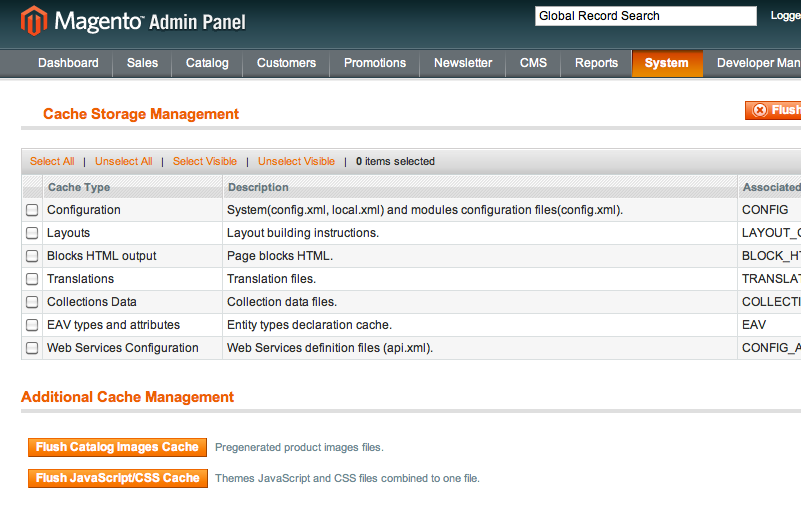
\includegraphics[width=1\textwidth]{images/appendix_f/cache-manage.png}
\end{center}
\caption{}
%\label{fig:awesome_image}
\end{figure}


From this page you can clear out the cache, or turn it off entirely.

Occasionally, a cached configuration may prevent you from getting to the Magento Admin Console.  For example, consider an event observer with an invalid class name.  If this happens, you'll want to look in the \footnotesize\texttt{var/cache} \normalsize  folder

\begin{lstlisting}
ls -l var/cache
total 0
drwxrwxrwx   10 _www  staff   340 Mar 15 16:10 mage--0
drwxrwxrwx   10 _www  staff   340 Mar 15 16:10 mage--1
drwxrwxrwx    6 _www  staff   204 Mar 15 16:02 mage--2
drwxrwxrwx    8 _www  staff   272 Mar 15 16:02 mage--3
drwxrwxrwx    8 _www  staff   272 Mar 15 16:10 mage--4
drwxrwxrwx   12 _www  staff   408 Mar 15 16:02 mage--5
drwxrwxrwx   10 _www  staff   340 Mar 15 16:02 mage--6
drwxrwxrwx    8 _www  staff   272 Mar 15 16:02 mage--7
drwxrwxrwx   12 _www  staff   408 Mar 15 16:02 mage--8
drwxrwxrwx   10 _www  staff   340 Mar 15 16:02 mage--9
drwxrwxrwx    6 _www  staff   204 Mar 15 16:02 mage--a
drwxrwxrwx   10 _www  staff   340 Mar 15 16:02 mage--b
drwxrwxrwx  164 _www  staff  5576 Mar 15 16:02 mage--c
drwxrwxrwx  172 _www  staff  5848 Mar 15 16:02 mage--d
drwxrwxrwx    4 _www  staff   136 Mar 15 16:10 mage--e
drwxrwxrwx   12 _www  staff   408 Mar 15 16:10 mage--f

\end{lstlisting}


This folder is where Magento stores its cached data. Delete everything in this folder to manually clear the Magento cache and restore you store's functionality.

\emph{Visit http://www.pulsestorm.net/nofrills-layout-appendix-f to join the discussion online.}
\chapter{Magento Setters and Getters}
In most MVC model systems a common pattern develops.  Developers find they need to store two general types of data

\begin{enumerate}
\item "Business Logic" data (ex. a product's SKU)
\item Data that allows the model to function (ex. the database table name)
\end{enumerate}


It's very common to see developers use a single \footnotesize\texttt{array} \normalsize  (or similar, hash table like structure) property to store the business logic data, allowing the other class/object properties to be used for system functionality.  Magento is no different.  Any object that comes from a class that inherits from \footnotesize\texttt{Varien\_Object} \normalsize  (which includes both models and blocks) has a protected \footnotesize\texttt{\$\_data} \normalsize  property

\begin{lstlisting}
/**
 * Object attributes
 *
 * @var array
 */
protected $_data = array();

\end{lstlisting}


This array holds all the object's business logic data.  You can get an array of key/value pairs for this data with the \footnotesize\texttt{getData} \normalsize  method.

\begin{lstlisting}
var_dump($object->getData());

\end{lstlisting}


If you want to \textbf{set} a specific data field, use

\begin{lstlisting}
$object->setData('the_key', 'value');

\end{lstlisting}


similarly, if you want a specific field back from an object, you can use

\begin{lstlisting}
$value = $object->getData('the_key');

\end{lstlisting}


and you can set multiple keys at once by using \footnotesize\texttt{setData} \normalsize  with an array.

\begin{lstlisting}
$value = $object->setData(array(
'the_key'=>'value'
'the_thing'=>$thing,
));

\end{lstlisting}


You've probably noticed we're naming our keys using an all lower-case, underscore-for-spaces convention.  While nothing enforces this, it \emph{is} the standard Magento convention.  Beyond consistency, this also helps when it comes to Magento's magic getter and setter methods.

\section{Getter and Setter}

In addition to the data getting and setting methods mentioned above, there's also a more "magic" syntax.

\begin{lstlisting}
$key = $object->getTheKey();
$object->setTheKey('value');

\end{lstlisting}


Using PHP's \footnotesize\texttt{\_\_call} \normalsize  method, Magento has implemented their own \footnotesize\texttt{get} \normalsize  and \footnotesize\texttt{set} \normalsize  methods.  If you call a method on an object (with \footnotesize\texttt{Varien\_Object} \normalsize in the inheritance chain) whose name begins with \footnotesize\texttt{get} \normalsize  or \footnotesize\texttt{set}\normalsize, \textbf{and} there isn't an existing method already with the same name, Magento will use the remainder of the method name to create a data property key, and either get or set the value.  That means this

\begin{lstlisting}
$object->setTheKey('value');

\end{lstlisting}


is equivalent to this

\begin{lstlisting}
$object->setData('the_key','value');

\end{lstlisting}


That's why it's important to keep with the lowercase/underscore key convention.  Magento will convert the leading-camel-case

\begin{lstlisting}
TheKey

\end{lstlisting}


into a key named

\begin{lstlisting}
the_key

\end{lstlisting}


Another neat feature here is that the \footnotesize\texttt{set} \normalsize  method will always return an instance of the object being set, which enables method chaining

\begin{lstlisting}
$object->setFoo('bar')->setBaz('hola')->save();

\end{lstlisting}


After using this style interface for a few weeks you'll be loath to return to typing out array brackets.

\section{Other Magic Methods}

Magento also has magic methods for unsetting, and checking for the existence of a property

\begin{lstlisting}
$this->unsTheKey();
$this->hasTheKey();

\end{lstlisting}


Checkout the source of \footnotesize\texttt{Varien\_Object} \normalsize  for more information

\begin{lstlisting}
public function __call($method, $args)
{
    switch (substr($method, 0, 3)) {
        case 'get' :
            //Varien_Profiler::start('GETTER: '.get_class($this).'::'.$method);
            $key = $this->_underscore(substr($method,3));
            $data = $this->getData($key, isset($args[0]) ? $args[0] : null);
            //Varien_Profiler::stop('GETTER: '.get_class($this).'::'.$method);
            return $data;

        case 'set' :
            //Varien_Profiler::start('SETTER: '.get_class($this).'::'.$method);
            $key = $this->_underscore(substr($method,3));
            $result = $this->setData($key, isset($args[0]) ? $args[0] : null);
            //Varien_Profiler::stop('SETTER: '.get_class($this).'::'.$method);
            return $result;

        case 'uns' :
            //Varien_Profiler::start('UNS: '.get_class($this).'::'.$method);
            $key = $this->_underscore(substr($method,3));
            $result = $this->unsetData($key);
            //Varien_Profiler::stop('UNS: '.get_class($this).'::'.$method);
            return $result;

        case 'has' :
            //Varien_Profiler::start('HAS: '.get_class($this).'::'.$method);
            $key = $this->_underscore(substr($method,3));
            //Varien_Profiler::stop('HAS: '.get_class($this).'::'.$method);
            return isset($this->_data[$key]);
    }
    throw new Varien_Exception("Invalid method " . get_class($this) . "::" .
    $method."(".print_r($args,1).")");
}

\end{lstlisting}


\emph{Visit http://www.pulsestorm.net/nofrills-layout-appendix-g to join the discussion online.}
\chapter{Widget Field Rendering Options}
The simplest configuration for a Magento widget data parameter is

\begin{lstlisting}
<parameters>
    <our_parameter>
        <visible>0</visible>
        <required>1</required>
        <value>foobazbar</value>
        <type>text</type>
    </our_parameter>
</parameters>

\end{lstlisting}


This creates a hidden field (\footnotesize\texttt{\textless visible\textgreater 0\textless /visible\textgreater }\normalsize) that will always be populated with the value 'foobazbar' (\footnotesize\texttt{\textless value\textgreater foobazbar\textless /value\textgreater }\normalsize).

While hidden fields are useful for widgets entered via a CMS content area, it's  far more common for parameters to have a visible user interface element that  allows end-system-users to enter data.  That is to say, a visible text field is more common

\begin{lstlisting}
<parameters>
    <our_parameter>
        <visible>1</visible>
        <required>1</required>
        <label>Label for our Parameter</label>
        <type>text</type>
        <value>bazbarfoo</value>
        <sort_order>10</sort_order>
    </our_parameter>
</parameters>

\end{lstlisting}


We've changed the \footnotesize\texttt{\textless visible/\textgreater } \normalsize  tag so it contains the value "1" (boolean for true).  We've also added a \footnotesize\texttt{\textless label\textgreater } \normalsize  tag which will be used as the text label which describes the field, and a \footnotesize\texttt{\textless sort\_order\textgreater } \normalsize  field which control where (above or below) a particular UI element will show up compared to others.  The \footnotesize\texttt{\textless value\textgreater bazbarfoo\textless /value\textgreater } \normalsize  tag will set the \textbf{default} value for the UI element.

\begin{figure}[htb]
\begin{center}
\leavevmode
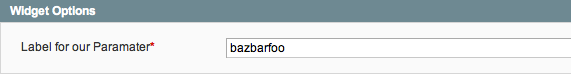
\includegraphics[width=1\textwidth]{images/appendix_g/field.png}
\end{center}
\caption{}
%\label{fig:awesome_image}
\end{figure}


You can also augment your fields with some instructional text by using the \footnotesize\texttt{\textless description/\textgreater } \normalsize  node.

\begin{lstlisting}
<parameters>
    <our_parameter>
        <visible>1</visible>
        <required>1</required>
        <label>Label for our Parameter</label>
        <type>text</type>
        <value>bazbarfoo</value>
        <sort_order>10</sort_order>
        <description>
            This is the field where we put the thing
        </description>
    </our_parameter>
</parameters>

\end{lstlisting}


Sometimes a free form text field gives users too much control over what values they enter in a widget.  For cases where we want to restrict a user's choices, we can use a \footnotesize\texttt{select} \normalsize  or \footnotesize\texttt{multiselect}\normalsize.

\begin{lstlisting}
<parameters>
    <our_parameter>
        <visible>1</visible>
        <required>1</required>
        <label>Should I Stay or Should I Go?</label>
        <type>select</type>
        <value>stay</value>
        <values>
            <staying>
                <value>stay</value>
                <label>There will be Trouble</label>
            </staying>
            <going>
                <value>go</value>
                <label>There will be Double</label>
            </going>
        </values>
        <sort_order>10</sort_order>
    </our_parameter>
</parameters>

\end{lstlisting}


The important changes here are we've changed our to \footnotesize\texttt{\textless type/\textgreater } \normalsize  tag to \footnotesize\texttt{select}\normalsize, and added a new \footnotesize\texttt{\textless values/\textgreater } \normalsize  node.  The sub-nodes of the \footnotesize\texttt{\textless values/\textgreater } \normalsize  node will be used to create the label/value pairs for the HTML \footnotesize\texttt{\textless select\textgreater } \normalsize  elements generated for the front end.  Alternatly, you can provide the name of a source model.

\begin{lstlisting}
<parameters>
    <our_parameter>
        <visible>1</visible>
        <required>1</required>
        <label>Should I Stay or Should I Go?</label>
        <type>select</type>
        <value>stay</value>
        <source_model>adminhtml/system_config_source_yesno</source_model>
        <sort_order>10</sort_order>
    </our_parameter>
</parameters>

\end{lstlisting}


The string \footnotesize\texttt{adminhtml/system\_config\_source\_yesno} \normalsize  is a class alias for a Magento model (in this case \footnotesize\texttt{Mage\_Adminhtml\_Model\_System\_Config\_Source\_Yesno}\normalsize). Source models are special model classes with a \footnotesize\texttt{toOptionArray} \normalsize  method.

\begin{lstlisting}
class Mage_Adminhtml_Model_System_Config_Source_Yesno
{

    /**
     * Options getter
     *
     * @return array
     */
    public function toOptionArray()
    {
        return array(
            array('value' => 1, 'label'=>Mage::helper('adminhtml')->__('Yes')),
            array('value' => 0, 'label'=>Mage::helper('adminhtml')->__('No')),
        );
    }

}

\end{lstlisting}


This method returns a set of key/value pairs for your select. You may create your own source models, or use one the models that ships with Magento.  Checkout the PHP files in

\begin{lstlisting}
app/code/core/Mage/Adminhtml/Model/System/Config/Source

\end{lstlisting}


for a list of the source models that ship with Magento.

\section{Creating Your Own Form Elements}

Sometimes you're going to want a form element that's more interactive than a single text or a select.  The widget system has a mechanism that allows you to build your own form elements for the widget UI.

First, your parameter configuration should look like the following

\begin{lstlisting}
<our_parameter>
    <visible>1</visible>
    <required>1</required>
    <label>Should I Stay or Should I Go?</label>
    <type>label</type>
    <helper_block>
        <type>yourpackage_yourmodule/widgettest</type>
    </helper_block>
    <sort_order>10</sort_order>
    <description>This is the field where you'll put the synergy.</description>
</our_parameter>

\end{lstlisting}


The key nodes here are \footnotesize\texttt{\textless type\textgreater } \normalsize  and \footnotesize\texttt{\textless helper\_block\textgreater }\normalsize.  Our field type here is \footnotesize\texttt{label}\normalsize.  Normally, a field type of label will render the label for a field without any form element.  In other words, a form element with no functional value, only instructional/branding/experience.  However, we've also included a \footnotesize\texttt{\textless helper\_block\textgreater } \normalsize  node.  This node (via the \footnotesize\texttt{\textless type/\textgreater } \normalsize  sub-node) configures a block class that will render our form.

After configuring this parameter, you'll need to define your block class.  Despite living in the standard block heirarchy, we \textbf{do not} want to implement our rendering in its \footnotesize\texttt{\_toHtml} \normalsize  method.  Instead, this class needs a special method named \footnotesize\texttt{prepareElementHtml} \normalsize

\begin{lstlisting}
#File: app/code/local/Yourpackage/Yourmodule/Block/Widgettest.php
class Yourpackage_Yourmodule_Block_Widgettest extends Mage_Core_Block_Abstract
{
    /**
    * Overly simple example
    */
    public function prepareElementHtml(
    Varien_Data_Form_Element_Abstract $element)
    {
        $simple_input = '<input type="text" name="' .
        strip_tags($element->getName()) .
        '" value="' .
        strip_tags($element->getValue()).
        '"/>';

        $element->setData('after_element_html', $simple_input);

        $element->setValue(''); //blank out value
        return $element;
    }
}

\end{lstlisting}


During the rendering of your parameter's UI, Magento will call the  \footnotesize\texttt{prepareElementHtml} \normalsize  method of your \footnotesize\texttt{helper\_block}\normalsize, passing in a \footnotesize\texttt{Varien\_Data\_Form\_Element\_Abstract} \normalsize  object.  This \footnotesize\texttt{\$element} \normalsize  is the object that Magento will use to render out your form element.  To implement a custom form element, your job is

\begin{enumerate}
\item Grab the form element's name and value from \footnotesize\texttt{\$element}\normalsize. The value will contain previously saved values, and the name will be the correct name for the HTML form element to ensure the form data is saved on post
\item Add HTML to the form element's rendering process to implement your custom element
\item Optionally, if you don't want the default value rendering to take place, clear the value from \footnotesize\texttt{\$element} \normalsize  before returning it.
\end{enumerate}


In our example above, we've created a ludicrously simple example to demonstrate how you might acheive this. We've

\begin{enumerate}
\item Created a HTML element \footnotesize\texttt{(\$simple\_input}\normalsize) using string concatenation.
\item Added this HTML to the element with \footnotesize\texttt{\$element-\textgreater setData('after\_element\_html', \$simple\_input);} \normalsize
\item Zeroed out the value of \footnotesize\texttt{\$element} \normalsize
\end{enumerate}


\section{Advanced Examples}

As mentioned, our example above is ludicrously simple.  However, with the power to create any arbitrary HTML, CSS or Javascript for your form, the possibilities are endless.  Look to a few of Magento's \footnotesize\texttt{\textless block\_helper\textgreater } \normalsize s for inspiration

\begin{lstlisting}
app/code/core/Mage/Adminhtml/Block/Catalog/Category/Widget/Chooser.php
app/code/core/Mage/Adminhtml/Block/Catalog/Product/Widget/Chooser.php
app/code/core/Mage/Adminhtml/Block/Cms/Block/Widget/Chooser.php
app/code/core/Mage/Adminhtml/Block/Cms/Page/Widget/Chooser.php

\end{lstlisting}


\emph{Visit http://www.pulsestorm.net/nofrills-layout-appendix-h to join the discussion online.}
\chapter{System Configuration Variables}
A simple system configuration system might store a set of key/value pairs something like this.

\begin{lstlisting}
$config['db_name']      = 'localhost';
$config['db_password']  = '12345';
$config['logo']         = 'awesomelogo.gif';
etc.

\end{lstlisting}


However, in keeping with its core philosophy of "When in doubt, use XML", Magento stores its system configuration values in \emph{tree} format.  The above might be represented something like this

\begin{lstlisting}
<system_config>
    <store>
        <database>
            <name>localhost</name>
            <password>12345</password>
        </databases>
        <design>
            <logo>awesomelogo.gif</logo>
        </design>
    </store>
</system_config>

\end{lstlisting}


This is a common approach to modern configuration systems, as it allows you to develop a hierarchy of organized values as more and more sections of your system or application become configurable.  What's really interesting is, using xpath-like expressions, you can still treat a node-based configuration system as a set of key/value pairs.  That's exactly how you fetch a Magento System Configuration value

\begin{lstlisting}
Mage::getStoreConfig('store/database/name');
Mage::getStoreConfig('store/database/password');
Mage::getStoreConfig('store/design/logo');

\end{lstlisting}


Magento allows each module to define new nodes for this configuration tree, as well as user interfaces for store owners to enter configuration values in the Admin Console under

\begin{lstlisting}
System -> Configuration

\end{lstlisting}


This system is beyond the scope of this book, but there's plenty of information online.  If you're interested, you can start reading here

\begin{lstlisting}
http://alanastorm.com/custom_magento_system_configuration

\end{lstlisting}


\emph{Visit http://www.pulsestorm.net/nofrills-layout-appendix-i to join the discussion online.}
\chapter{Magento Connect}
Magento Connect is a lot of things.  First and foremost, it's Magento Inc's online repository for free, downloadable extensions.  It's also a package management system that was, originally, based on the PHP PEAR packaging format.  Magento Connect 2.0 was released along with Magento CE 1.5.  This means there's two separate package file formats, which is why we've included two different sets of modules.

\section{What is an Extension}

As you may already know, Magento separates its "backend" code into formal code modules. A Magento Connect extension may \textbf{contain} modules, but a Magento Connect extension is not \textbf{just} a code module.

A Magento Connect extension is a packaged collection of files that Magento will install into your system.  Each file in the package has a Magento Connect type, which will control where Magento installs the file.  For example, a \textbf{local module file} knows to install itself in \footnotesize\texttt{./app/code/local}\normalsize, whereas a \textbf{PHP Library file} installs itself in \footnotesize\texttt{./lib}\normalsize.  See

\begin{quote}
System -\textgreater  Connect -\textgreater  Package Extensions
\end{quote}

for a full list of types.

There's one type in particular you'll want to be aware of.  That's the \textbf{other} type.  This type's base folder is Magento's base installation folder, which gives a Magento extension the ability to install a file \textbf{anywhere} in your system, and in turn you can create a package that includes files from anywhere.

\section{Installing Extensions: The GUI Way}

There's a GUI admin for Magento Connect.  You can reach it from the Admin Console by navigating to

\begin{lstlisting}
System -> Magento Connect -> Magento Connect Manager

\end{lstlisting}


You'll need to reauthorize your session as the admin user, (or any user with Magento Connect ACL rights).  The code that bootstraps the Magento Connect Manager is separate from the source code of your Magento system proper.

Installing extensions that have been uploaded to Magento Inc's central server is as easy as entering the extension key into the installation field.

If you've downloaded a \footnotesize\texttt{.tgz} \normalsize  package file from the internet, Magento 1.5 also offers a handy upload form, allows you to directly upload an extension

\section{Installing Extensions: The Command Line Way}

Both the 1.4x and 1.5x branches of Magento offer the ability to install extension from the command line.  However, the tools used for each version differ slightly.

\subsection{Magento Connect CLI install for Magento 1.42}

In the root folder of Magento 1.4.2 there's a shell script named \footnotesize\texttt{pear}\normalsize.  This shell script in \textbf{not} the standard PEAR installer.  It's a customized installer you may use to install Magento Connect extensions.  To use it, you'll need to tell your operating system its allowed to execute it as a program

\begin{lstlisting}
chmod +x pear

\end{lstlisting}


After that, you'll need to run

\begin{lstlisting}
./pear mage-setup

\end{lstlisting}


After setting a number of configuration variables and initializing two channels

\begin{lstlisting}
connect.magentocommerce.com/core
connect.magentocommerce.com/community

\end{lstlisting}


the script will exit.  You're now ready to install and uninstall packages using the command line installer

\begin{lstlisting}
./pear install No_Frills_Magento_Layout_1_start-1.0.0.tgz
./pear uninstall \
channel://connect.magentocommerce.com/community/No_Frills_Magento_Layout_1_sta...

\end{lstlisting}


\subsection{Magento Connect CLI install for Magento 1.5+}

Magento 1.5 removed the \footnotesize\texttt{pear} \normalsize  installer, and introduced a new command line script (\footnotesize\texttt{mage}\normalsize) that offers a similar function.  Again, you'll need to give it executable permissions

\begin{lstlisting}
chmod +x mage

\end{lstlisting}


and then initialize it with

\begin{lstlisting}
./mage mage-setup

\end{lstlisting}


After the setup script finishes running, you'll be able to install extensions from a file. \textbf{NOTE}: The command has changed to \footnotesize\texttt{install-file}\normalsize, and the arguments to uninstall have changed as well

\begin{lstlisting}
./mage install-file No_Frills_Magento_Layout_3_start-1.0.0.tgz
./mage uninstall community No_Frills_Magento_Layout_3_start

\end{lstlisting}


\emph{Visit http://www.pulsestorm.net/nofrills-layout-appendix-j to join the discussion online.}

%\chapter{Introduction}
%\input{var/0_intro}
%
%reference
%\chapter{Introduction}
%Lorem \emph{ipsum dolor sit amet}, consectetur \textbf{adipisicing elit}, sed do eiusmod tempor incididunt ut labore et dolore magna aliqua. Ut enim ad minim veniam, quis nostrud exercitation ullamco laboris nisi ut aliquip ex ea commodo consequat. Duis aute irure dolor in reprehenderit in voluptate velit esse cillum dolore eu fugiat nulla pariatur. Excepteur sint occaecat cupidatat non proident, sunt in culpa qui officia deserunt mollit anim id est laborum.
%\chapter{Foo Baz Bar}
%Lorem \emph{ipsum dolor sit amet}, consectetur \textbf{adipisicing elit}, sed do eiusmod tempor incididunt ut labore et dolore magna aliqua. Ut enim ad minim veniam, quis nostrud exercitation ullamco laboris nisi ut aliquip ex ea commodo consequat. Duis aute irure dolor in reprehenderit in voluptate velit esse cillum dolore eu fugiat nulla pariatur. Excepteur sint occaecat cupidatat non proident, sunt in culpa qui officia deserunt mollit anim id est laborum.
%\begin{figure}[htb]
%\begin{center}
%\leavevmode
%\includegraphics[width=1\textwidth]{../images/chapter1/twocities}
%\end{center}
%%\caption{Screen Shot}
%%\label{fig:awesome_image}
%\end{figure}
%\section{A Section Header}
%Lorem ipsum dolor sit amet, consectetur adipisicing elit, sed do eiusmod tempor incididunt ut labore et dolore magna aliqua. Ut enim ad minim veniam, quis nostrud exercitation ullamco laboris nisi ut aliquip ex ea commodo consequat. Duis aute irure dolor in reprehenderit in voluptate velit esse cillum dolore eu fugiat nulla pariatur. Excepteur sint occaecat cupidatat non proident, sunt in culpa qui officia deserunt mollit anim id est laborum.
%\subparagraph{The quick brown fox jumps over the lazy dog.}
%\chapter{Building Layouts Programmatically}
%Lorem ipsum dolor sit amet, consectetur adipisicing elit, sed do eiusmod tempor incididunt ut labore et dolore magna aliqua. Ut enim ad minim veniam, quis nostrud exercitation ullamco laboris nisi ut aliquip ex ea commodo consequat. Duis aute irure dolor in reprehenderit in voluptate velit esse cillum dolore eu fugiat nulla pariatur. Excepteur sint occaecat cupidatat non proident, sunt in culpa qui officia deserunt mollit anim id est laborum.
%\appendix
%\chapter{Awesome}
%Lorem ipsum dolor sit amet, consectetur adipisicing elit, sed do eiusmod tempor incididunt ut labore et dolore magna aliqua. Ut enim ad minim veniam, quis nostrud exercitation ullamco laboris nisi ut aliquip ex ea commodo consequat. Duis aute irure dolor in reprehenderit in voluptate velit esse cillum dolore eu fugiat nulla pariatur. Excepteur sint occaecat cupidatat non proident, sunt in culpa qui officia deserunt mollit anim id est laborum.
%\chapter{Foo Baz Bar}
%Lorem ipsum dolor sit amet, consectetur adipisicing elit, sed do eiusmod tempor incididunt ut labore et dolore magna aliqua. Ut enim ad minim veniam, quis nostrud exercitation ullamco laboris nisi ut aliquip ex ea commodo consequat. Duis aute irure dolor in reprehenderit in voluptate velit esse cillum dolore eu fugiat nulla pariatur. Excepteur sint occaecat cupidatat non proident, sunt in culpa qui officia deserunt mollit anim id est laborum.


\end{document}